
\section{Über dieses Dokument}
\label{sec:org502edb3}

Im nachfolgenden Abschnitt finden Sie allgemeine Informationen zu
diesem Dokument.

\subsection{Beschreibung}
\label{sec:org19761cf}

Diese Arbeit hat zum Ziel, die Planung und Erstellung einer grafischen
Oberfläche zum einfachen Bedienen der Software \gls{borg} \footcite{borgbackup} ,
durchzuführen sowie zu dokumentieren.

\subsection{Zweck und Inhalt}
\label{sec:org1f0870e}

Zweck dieses Dokumentes ist die vollständige und nachvollziehbare Dokumentation
zur Diplomarbeit von Andreas Zweili.

\subsection{Aufbau}
\label{sec:org5e29840}

Alle Inhalte sind in der Regel chronologisch sortiert, vom ältesten zum jüngsten
Ereignis, und nach Kapiteln getrennt. An gewissen Stellen kann die
chronologische Reihenfolge allenfalls nicht gewährleistet werden.

\subsection{Lizenz}
\label{sec:org6aaf06a}

Dieses Dokument wurde von Andreas Zweili im Rahmen der Diplomarbeit an der IBZ
Schule erstellt und steht unter der \gls{cc} BY-SA 4.0 \footcite{cc} Lizenz.
Dadurch darf die Arbeit unter Beibehalten der Lizenz kopiert und
weiterverarbeitet werden. Zusätzlich muss der Urheber genannt werden.

\section{Initialisierung}
\label{sec:org4bffdd1}
\subsection{Vision}
\label{sec:org2a2aa21}

Die Software soll \gls{borg} für den durchschnittlichen Computer User zugänglich
machen. Backups sollen dabei schnell und unkompliziert erstellt werden können.
Auch die Möglichkeit automatischer im Hintergrund laufender Backups soll dem
User gegeben sein, damit die Hürde für Backups so tief wie möglich gehalten
wird.

Die besten Backups sind solche, bei denen man gar nicht mehr weiss das man sie
hat, bis man sie braucht.

\subsection{Ausgangslage}
\label{sec:org6dd617e}

\gls{borg} ist deshalb interessant, weil es während einem Backup relativ
wenig Ressource im Vergleich zu anderen Systemen benötigt und schon relativ
lange aktiv entwickelt wird. Dadurch ist es im Alltag geprüft worden.
Des Weiteren bietet \gls{borg} die Funktion für Verschlüsselung was es einem User
ermöglicht die Daten auf einem unsicheren Cloud Speicher abzulegen.

Des Weiteren speichert \gls{borg} die Daten mit Block basierter \gls{dedup} ab. Dies
hat den riesigen Vorteil das bei einem Backup nur die Änderungen auf
Block-Ebene gespeichert werden und nicht jedes Mal die ganze Datei kopiert
werden muss.

Damit ermöglicht die Software auch Backups von sehr grossen Dateien, wie Videos
oder Disk Images von virtuellen Maschinen, in mehreren Versionen. Ohne dabei
jedoch signifikant mehr an Speicher zu benötigen. Zusätzlich werden die Backups
dadurch rasend schnell ausgeführt. Gerade dieses Feature macht \gls{borg} in den
Augen des Autors besonders interessant da sich der durchschnittliche User
möglichst wenig mit Dingen wie Backups auseinandersetzen möchte. Umso besser
also, wenn sie schnell gehen und so wenig Speicherplatz wie möglich verbrauchen.

\gls{borg} wird jedoch komplett über die Kommandozeile bedient. Somit ist es für
normale Benutzer eher schwierig den Zugang zu der Software zu finden geschweige
denn sie zu bedienen.

\gls{borg} bietet Entwicklern eine \gls{json}, \gls{api}, mit welcher sie, von \gls{borg}
ausgegebenen Dateien einfach weiterverarbeiten können.

\gls{borg} steht unter einer \gls{bsd} \footcite{bsd} Lizenz zur Verfügung und ist somit
\gls{libre}.

Das Projekt muss dabei vom Studenten in Eigenarbeit und einer Zeit von 250
Stunden bis zum 18. März 2019 erarbeitet werden.

\subsection{Projektziele}
\label{sec:orgbc17b07}

Das Hauptziel der Arbeit soll es sein eine einfach nutzbare grafische
Oberfläche für \gls{borg} zu entwickeln. Da \gls{borg} selber freie Software ist und
der Autor mit \gls{libre} viel gute Erfahrungen gemacht hat, soll das Projekt
selber auch wieder \gls{libre} sein. Zum einen um der Community etwas
zurückzugeben des weiteren, um anderen Entwicklern die Möglichkeit zu geben die
Software zu verbessern und weiter zu entwickeln.

Als neben läufiges Ziel soll mit dieser Arbeit auch die Verbreitung von freier
Software gefördert werden. Dies wird insbesondere dadurch erreicht, dass die
Software selbst unter der \gls{gpl} Version 3 \footcite{gplv3}
veröffentlicht wird. Wenn möglich sollen während der Entwicklung auch
hauptsächlich freie Software verwendet werden. Die gesamte Arbeit wird zudem zu
jedem Zeitpunkt öffentlich einsehbar sein. Der Quelltext der Dokumentation ist
unter diesem Link erreichbar: \url{https://git.2li.ch/Nebucatnetzer/thesis}

Die Entwicklung wird hauptsächlich auf einem Linux System stattfinden. Da
\gls{borg} einerseits hauptsächlich auf Unix Systeme ausgelegt ist und
anderseits die Hauptzielgruppe des Projektes auch auf Linux Usern liegt.
Trotzdem sollen im Projekt cross-plattform fähige Technologien eingesetzt werden
damit es in der Zukunft möglich ist das Projekt auf andere Plattformen
auszuweiten.

\subsubsection{Ziele inklusive Gewichtung}
\label{sec:orgfaaeb2b}

Im Projektantrag wurden vor gängig folgende Ziele definiert und entsprechend
gewichtet. Die Gewichtung wurde dabei so vorgenommen, dass Ziele mit einer
Muss-Gewichtung den Minimalanforderungen der Software entsprechen. Die weiteren
Ziele wurden dann mit Ziffern von 5 bis 1 gewichtet. Eine 5 bedeutet dabei
dass, das Ziel in naher Zukunft sehr nützlich/wichtig für die Software wäre
ist. Eine tiefe Zahl sollte dabei, wenn möglich, auch einmal in die Software
integriert werden und ist nicht unwichtig.

\begin{longtable}{|p{1cm}|p{9cm}|p{1.5cm}|p{2cm}|}
\hline
\textbf{Ziel-Nr.}\cellcolor[HTML]{C0C0C0} & \textbf{Zielsetzung}\cellcolor[HTML]{C0C0C0} & \textbf{Muss}\cellcolor[HTML]{C0C0C0} & \textbf{Wunsch}\newline (1-5, 5=sehr wichtig)\cellcolor[HTML]{C0C0C0}\\
\hline
\endfirsthead
\multicolumn{4}{l}{Fortsetzung von vorheriger Seite} \\
\hline

\textbf{Ziel-Nr.}\cellcolor[HTML]{C0C0C0} & \textbf{Zielsetzung}\cellcolor[HTML]{C0C0C0} & \textbf{Muss}\cellcolor[HTML]{C0C0C0} & \textbf{Wunsch}\newline (1-5, 5=sehr wichtig)\cellcolor[HTML]{C0C0C0} \\

\hline
\endhead
\hline\multicolumn{4}{r}{Fortsetzung nächste Seite} \\
\endfoot
\endlastfoot
\hline
1. & Die Anwendung setzt auf cross-plattform (Linux, Windows, OS X) fähige Technologien. & x & \\
\hline
2. & Die Anwendung steht unter der \gls{gpl} v3 der Öffentlichkeit zur Verfügung. & x & \\
\hline
3. & Der User kann mit weniger als 3 Klicks ein Backup ausführen. & x & \\
\hline
4. & Der User kann ein Archiv mit 3 Klicks löschen. & x & \\
\hline
5. & Der User kann unter Linux ein Archiv mit zwei Klicks "`red-only"' als Laufwerk mounten. & x & \\
\hline
6. & Der User kann ein Archiv wieder herstellen. & x & \\
\hline
7. & Der User kann den zu sichernden Pfad manuell in der Anwendung definieren. & x & \\
\hline
8. & Die Applikation holt ihre Konfiguration aus einer Plain-Text Datei. & x & \\
\hline
9. & Der User kann sein Repository auf einer Harddisk ablegen. & x & \\
\hline
10. & Die Anwendung exkludiert für einen Linux Computer sinnvolle Pfade bereits zu Beginn. & x & \\
\hline
11. & Die Archivliste wird nach einer Aktion automatisch aktualisiert. & x & \\
\hline
12. & Der User kann sein Repository auf einem über SSH erreichbaren Server ablegen. &  & 5\\
\hline
13. & Der User kann den Namen eines Archivs selbst bestimmen. &  & 5\\
\hline
14. & Die Anwendung meldet transparent, wenn das Repository nicht erreichbar ist. &  & 5\\
\hline
15. & Die Anwendung meldet dem User, wenn noch ein Hypervisor am Laufen ist. &  & 5\\
\hline
16. & Die Anwendung leitet Meldungen von \gls{borg} transparent weiter. &  & 5\\
\hline
17. & Die Anwendung zeigt transparent an das \gls{borg} im Hintergrund bereits läuft. &  & 5\\
\hline
18. & Das Repository wird nach jedem Backup bereinigt. &  & 4\\
\hline
19. & Der User kann automatische Hintergrundbackups in der Anwendung konfigurieren. &  & 4\\
\hline
20. & Die Anwendung gibt dem User die Möglichkeit ein passendes Repository zu erstellen, wenn keines gefunden wird, die Anwendung jedoch bereits konfiguriert ist. &  & 4\\
\hline
21. & Die Applikation verwendet, wann immer möglich allgemeingültige Umgebungsvariablen. &  & 4\\
\hline
22. & Die Anwendung cached/speichert (evtl. zusätzliche) Informationen in einer Datenbank. &  & 3\\
\hline
23. & Die Anwendung zeigt beim ersten Starten einen Setup Wizard. &  & 3\\
\hline
24. & Der User kann sich mit 3 Klicks das Log eines Archivs anschauen. Nur möglich mit einer zusätzlichen DB. &  & 3\\
\hline
25. & Die Anwendung kann Systembenachrichtigungen auslösen. &  & 3\\
\hline
26. & Der User kann die Anwendung grafisch konfigurieren. &  & 3\\
\hline
27. & Der User kann entscheiden ob, ein gemountetes Archiv nach dem Schliessen der Applikation noch weiter verfügbar ist. &  & 2\\
\hline
28. & Der User kann das Repository wechseln. &  & 2\\
\hline
29. & Der User kann ein Archiv nach einer Datei oder einem Ordner durchsuchen. &  & 2\\
\hline
30. & Der User kann die "`Retention Policy"' konfigurieren. &  & 2\\
\hline
31. & Die Anwendung kann mit allen Features von \gls{borg} umgehen. &  & 2\\
\hline
32. & Die Applikation prüft, ob sie sich im richtigen Netzwerk befindet bevor sie eine Verbindung zum Server aufbaut. &  & 2\\
\hline
\caption{\label{tab:org47ae745}
Projektziele}
\\
\end{longtable}
\newpage

\subsection{Projektabgrenzung}
\label{sec:org6efbb72}

Die Anwendung beschränkt sich darauf Funktionen von \gls{borg} grafisch
darzustellen oder nützlich zu erweitern soweit dies über die \gls{api} möglich
ist. Wie in Abbildung:(\ref{fig:orgfa0d0f8}) zu sehen ist, werden die Aktionen effektiv
immer vom Borg Binary ausgeführt und nicht von der grafischen Oberfläche. Eine
Erweiterung von \gls{borg} ist nicht vorgesehen. Backup und Verschlüsselung sind
heikle Themen und sollten unbedingt nur von Experten angegangen werden. Das
Potenzial für Fehler und die Auswirkungen derer, sind einfach schlicht zu gross.

Des Weiteren wird die Grundlage für eine kollaborative Entwicklung geschaffen.
Während der Laufzeit der Diplomarbeit werden jedoch keine Inputs aus der Borg
Community im Bezug auf die Entwicklung entgegengenommen.

Bugs von \gls{borg} welche während der Dauer der Diplomarbeit vom Studenten
entdeckt werden, wird dieser dem Projekt melden jedoch nicht selber beheben.

\begin{figure}[htbp]
\centering
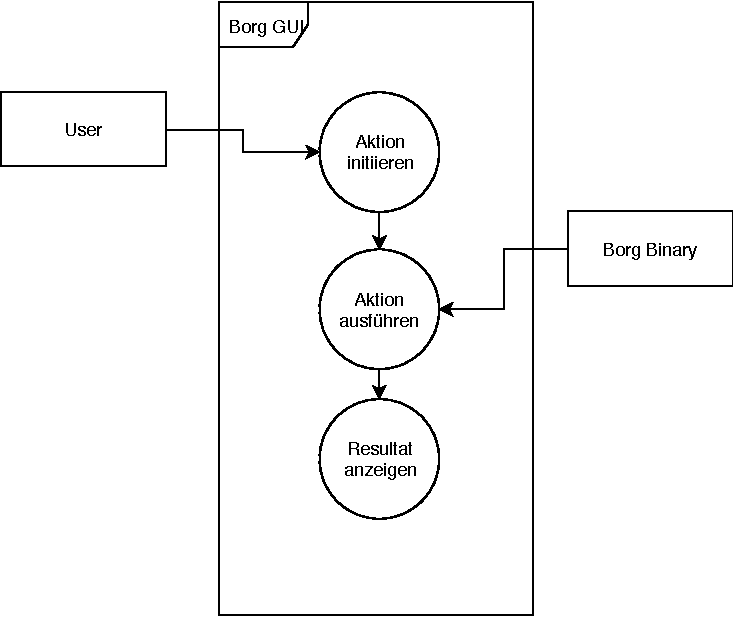
\includegraphics[width=.9\linewidth]{pictures/kontextdiagramm.pdf}
\caption{\label{fig:orgfa0d0f8}
Kontextdiagramm des Borg GUI}
\end{figure}

\subsection{Projektmethode}
\label{sec:orgb853aca}

Für das Projekt wurde die Wasserfall-Methode gewählt. Da nur eine
einzige Person am Projekt arbeitet, kann nur ein Task nach dem anderen
abgearbeitet werden und viele Aufgaben stehen in Abhängigkeiten zueinander.
Somit macht das iterative Vorgehen der Wasserfall-Methode für dieses Projekt am
meisten Sinn.

\subsection{Konfigurationsmanagement}
\label{sec:orgbbfcc86}

In der nachfolgenden Sektion wird definiert wie die Software und Dokumentation
versioniert wird und welche allgemeinen Werkzeuge eingesetzt werden.

\subsubsection{Versionskontrolle}
\label{sec:org6fa8ac3}

Die komplette Dokumentation, der Quellcode der Applikation sowie jegliche
zusätzlichen Dokumente wie etwa die Zeitplanung werden mittels der Software Git
versioniert. Thematisch zusammengehörende Änderungen werden in einem Commit
zusammengefasst. Somit ist jederzeit nachvollziehbar was wann geändert hat. Ein
Commit sollte dabei gemäss dem Artikel von Chris Beams "`How to write a Git
Commit Message"' \footcite{commit} und in englischer Sprache geschrieben sein.

Versionsnummern sind für die Applikation zum jetzigen Zeitpunkt noch nicht
vorgesehen. Sollten sie zukünftig einmal verwendet werden soll eine semantische
Versionierung \footcite{semver} verwendet. Dabei ist eine Versionsnummer immer
nach diesem Schema aufgebaut, MAJOR.MINOR.PATCH. Bei Änderungen wir die:
\begin{enumerate}
\item MAJOR Version erhöht, wenn man inkompatible Änderungen an der \gls{api} macht.
\item MINOR Version erhöht, wenn man Funktionalität hinzufügt, die
abwärtskompatibel ist.
\item PATCH Version erhöht, wenn man abwärtskompatibel Bug-Fixes hinzufügt.
\end{enumerate}

Auf jeden Fall sollte, wenn möglich immer nur lauffähiger Code im Master Branch
eingecheckt sein damit der Master Branch immer eine funktionierende Software
repräsentiert. Dies gilt auch für das Repository der Dokumentation. Der Master
Branch der Dokumentation sollte maximal mit zwei Befehlen \texttt{make clean} und
\texttt{make} "`kompilierbar"' sein.

Als Software für die Versionskontrolle wurde Git \footcite{git} aus folgenden
Gründen ausgewählt:

\begin{itemize}
\item Ist der de facto Standard bei Versionskontrollsoftware
\item Läuft auf allen gängigen Betriebssystemen
\item Es gäbe gratis Services, die man nutzen könnte (Github, Gitlab)
\item Man kann offline arbeiten und Commits erstellen
\item Der Autor hat bereits einen eigenen Git Server zur Verfügung
\item Der Autor ist bereits mit Git aus vorhergehenden Projekten vertraut,
dadurch muss man keine Ressourcen aufwenden eine neue Software zu lernen.
Zusätzlich hat sich Git in den vorhergehenden Projekten als robuste
und schnelle Software erwiesen.
\item Git ist \gls{libre} unter der \gls{gpl} v2.
\end{itemize}

\subsubsection{Editor}
\label{sec:orga862976}

Sowohl bei der Dokumentation wie auch bei der Programmierung wurde
hauptsächlich der Editor GNU Emacs \footcite{emacs} verwendet. GNU Emacs ist mit
32 Jahren (obwohl seine Wurzeln bis ins Jahre 1976 zurückgehen) wohl eines der
ältesten noch aktiven Software Projekte. Emacs ist \gls{libre} unter der
\gls{gpl} v3. Emacs wurde gewählt da es ein schneller, schlanker und sehr
flexibler Texteditor ist. Von normaler Textmanipulation über Taskmanagement
und Emails schreiben ist alles möglich.

\subsubsection{Dokumentation}
\label{sec:orgba2d6cf}

Diese Dokumentation wurde in Org-mode \footcite{orgmode}, einer Erweiterung für
den Text Editor Emacs, geschrieben. Die Syntax erinnert an Markdown und
Org-mode bietet einem eine Vielzahl an Hilfen dafür inklusive dem Erstellen von
Tabellen und Spreadsheet Funktionen. Für finale Version des Dokuments kann
Org-mode die ursprünglich Textdatei über \LaTeX{} in ein PDF exportieren.

\LaTeX{} \footcite{latex} ist eine Software, welche einem die Benutzung des
Textsatzsystems TeXs vereinfacht. \LaTeX{} wurde gegenüber einem "`What You See Is
What You Get"' (z.Bsp. MS. Word) Editor gewählt, weil es einem mit seiner Markup
Sprache erlaubt das Dokument in Text Dateien zu erstellen, gerade für
Programmiere ist dies eine sehr interessante Lösung. Dadurch, dass \LaTeX{} auch
nur aus reinen Textdateien besteht, kann man die Dokumente auch ohne weiteres
in die Versionskontrollsoftware einchecken und die Entwicklung im Log
zurückverfolgen. \LaTeX{} ist \gls{libre} unter der \LaTeX{} Project Public
License.

Die Grafiken in diesem Dokument wurden hauptsächlich mit dem Vektor Grafik
Editor Inkscape \footcite{inkscape} erstellt. Inkscape ist \gls{libre} unter der
GNU Public License v3.

Die Diagramme wurden mit Draw.io \footcite{draw} erstellt. Draw.io ist \gls{libre}
unter Apache Lizenz Version 2.0 \footcite{apache} und kann sowohl als Desktop
Applikation wie auch als Webanwendung genutzt werden.

Beim Design der Arbeit wurden soweit als möglich die typographischen Regeln aus
dem Buch "`Practical Typography"' von Matthew Butterick \footcite{typo} angewandt.
Bei den Diagrammen wurden ausschliesslich Farben aus der von Google
entwickelten Design Sprache "`Material"' \footcite{material} eingesetzt.

\subsection{Zeitplanung}
\label{sec:org013b6ac}

Die detaillierte Zeitplanung ist dem Ganttchart in der Datei
\href{Zeitplanung\_Andreas\_Zweili.html}{Zeitplanung\_Andreas\_Zweili.html} zu entnehmen. Bei der Zeitplanung wurde darauf
geachtet das die Arbeit soweit, als möglich nicht mit dem Berufsleben
kollidiert. An einem normalen Arbeitstag wurde dabei damit gerechnet das ca. 2
Stunden Arbeit am Abend möglich sein sollten. An einem arbeitsfreien Tag wurde
mit 6 Stunden Arbeit gerechnet. Über die Festtage wurden diverse Tage von der
Planung ausgenommen, da es nicht realistisch schien, dass an diesen Tagen die
Arbeit signifikant vorwärts gehen würde. Auch Schultage wurde nicht, als
Arbeitstage gerechnet da man meist nicht mehr für weitere Tätigkeiten gross
motiviert ist.

Als zusätzliche Massnahme um die Arbeitslast zu verteilen wurde vom 14. Januar
bis zum 11. März jeder Montag auf der Arbeitsstelle als frei eingegeben.
Dadurch steht, während des Projektes etwas mehr Zeit zur Verfügung als sonst mit
einer 100 Prozent Arbeitsstelle möglich wäre.

\subsection{Controlling}
\label{sec:orge0e7ff0}

Das Controlling wird verwendet, um zu kontrollieren, dass die eigentliche
Planung mit dem effektiv geleisteten Aufwand respektive den effektiv
verwendeten Ressourcen übereinstimmt. Somit können für zukünftige Projekte
Lehren gezogen werden.

\newpage
\begin{landscape}
\subsubsection{Zeitaufwand}
\label{sec:org94d76ba}

\begin{longtable}{|p{3cm}|p{5cm}|p{3cm}|p{7cm}|}
\hline
\textbf{Aufgabe}\cellcolor[HTML]{C0C0C0} & \textbf{Gesch. Aufwand}\cellcolor[HTML]{C0C0C0} & \textbf{Effekt. Aufwand}\cellcolor[HTML]{C0C0C0} & \textbf{Begründung}\cellcolor[HTML]{C0C0C0}\\
\hline
\endfirsthead
\multicolumn{4}{l}{Fortsetzung von vorheriger Seite} \\
\hline

\textbf{Aufgabe}\cellcolor[HTML]{C0C0C0} & \textbf{Gesch. Aufwand}\cellcolor[HTML]{C0C0C0} & \textbf{Effekt. Aufwand}\cellcolor[HTML]{C0C0C0} & \textbf{Begründung}\cellcolor[HTML]{C0C0C0} \\

\hline
\endhead
\hline\multicolumn{4}{r}{Fortsetzung nächste Seite} \\
\endfoot
\endlastfoot
\hline
\hline
 & \textbf{Gesamter Aufwand} &  & \\
\hline
\caption{\label{tab:orgc31fd34}
Zeitcontrolling}
\\
\end{longtable}
\end{landscape}

\subsubsection{Ressourcen}
\label{sec:org6914ce3}

Folgende Ressourcen werden während der Arbeit benötigt:
\begin{longtable}{|p{4cm}|p{2cm}|p{2cm}|p{4cm}|}
\hline
\textbf{Ressource}\cellcolor[HTML]{C0C0C0} & \textbf{geschätzte Stück}\cellcolor[HTML]{C0C0C0} & \textbf{effekt. Stück}\cellcolor[HTML]{C0C0C0} & \textbf{Begründung}\cellcolor[HTML]{C0C0C0}\\
\hline
\endfirsthead
\multicolumn{4}{l}{Fortsetzung von vorheriger Seite} \\
\hline

\textbf{Ressource}\cellcolor[HTML]{C0C0C0} & \textbf{geschätzte Stück}\cellcolor[HTML]{C0C0C0} & \textbf{effekt. Stück}\cellcolor[HTML]{C0C0C0} & \textbf{Begründung}\cellcolor[HTML]{C0C0C0} \\

\hline
\endhead
\hline\multicolumn{4}{r}{Fortsetzung nächste Seite} \\
\endfoot
\endlastfoot
\hline
Projektleiter/Mitarbeiter & 1 & 1 & keine Abweichung\\
Diplombetreuer & 1 & 1 & keine Abweichung\\
Testuser & 5 & 5 & keine Abweichung\\
Korrekturleser & 3 & 3 & keine Abweichung\\
iPad & 1 & 1 & keine Abweichung\\
Notebook & 1 & 1 & keine Abweichung\\
\hline
\caption{\label{tab:orge797eb6}
Ressourcen}
\\
\end{longtable}

\subsubsection{Kosten}
\label{sec:orgb1ea25c}

Werden die internen Lohnkosten des Projektleiters auf ca. 60 CHF pro Stunde
geschätzt, ergeben sich gemäss der Berechnung in der Tabelle:(\ref{tab:org1f6d821}),
theoretische Kosten von 19'200 CHF für die Umsetzung dieser Arbeit. Die Kosten
für die Entwicklung werden im Projekt jedoch nicht berücksichtigt, somit sind
die Kosten nur ein rein theoretischer Faktor.
\begin{table}[htbp]
\centering
\begin{tabular}{|l|c|c|r|}
\hline
\textbf{Name}\cellcolor[HTML]{C0C0C0} & \textbf{Aufwand in h}\cellcolor[HTML]{C0C0C0} & \textbf{Kosten in CHF}\cellcolor[HTML]{C0C0C0}\\
\hline
Initialisierung & 24 & 1440\\
Analyse & 47 & 2820\\
Konzept & 34 & 2040\\
Realisierung & 172 & 10320\\
Ausblick & 8 & 480\\
Arbeit korrigieren & 20 & 1200\\
Meeting \#1 & 5 & 300\\
Meeting \#2 & 5 & 300\\
Meeting \#3 & 5 & 300\\
\hline
\textbf{Total} & 320 & 19200\\
\hline
\end{tabular}
\caption{\label{tab:org1f6d821}
Kostenrechnung}

\end{table}

\subsection{Projektrisiken}
\label{sec:orgfb728f9}

Das Risikomanagement dient dazu Risiken im Projekt zu erkennen und Massnahmen
zur Vermeidung der Risiken zu definieren. Dadurch steht man ihnen nicht
unvorbereitet gegenüber, sollten sie eintreffen.

\subsubsection{Risikobeschreibung}
\label{sec:org6b04b96}

In der Tabelle: (\ref{tab:org5188bca}), sind die Risiken des Projektes
gemeinsam mit ihren Gegenmassnahmen aufgelistet. Somit können gewisse Risiken
bereits vorher abgefangen werden.

\begin{longtable}{|p{0.45\textwidth}|p{0.45\textwidth}|}
\hline
\textbf{Beschreibung}\cellcolor[HTML]{C0C0C0} & \textbf{Massnahmen}\cellcolor[HTML]{C0C0C0}\\
\hline
\endfirsthead
\multicolumn{2}{l}{Fortsetzung von vorheriger Seite} \\
\hline

\textbf{Beschreibung}\cellcolor[HTML]{C0C0C0} & \textbf{Massnahmen}\cellcolor[HTML]{C0C0C0} \\

\hline
\endhead
\hline\multicolumn{2}{r}{Fortsetzung nächste Seite} \\
\endfoot
\endlastfoot
\hline
Ein grösseres Problem in der Programmierung blockiert den Fortschritt. & Immer nur eine Sache auf einmal in der Code-Basis ändern, alle Fehler beheben und erst dann zur nächsten Aufgabe weitergehen.\\
\hline
Viel Arbeit an der Arbeitsstelle, dabei bleibt weniger Zeit für die Diplomarbeit. & Auf der Arbeit Freitage eingeben um die Last etwas zu verteilen. Projektplanung machen.\\
\hline
Know-How zur Umsetzung ist nicht vollständig vorhanden. & Gute Informationsbeschaffung im Internet, Büchern, etc.\\
\hline
Manuelle Tests brauchen zu viel Zeit. & Soviel wie möglich automatisieren. Dabei jedoch nicht den Fokus auf die eigentliche Entwicklung verlieren.\\
\hline
Die Programmierung des Programms benötigt zu viel Zeit. & Bei der Projektplanung genau definieren was die GUI Applikation beinhalten muss. Ziele definieren, Abgrenzungen treffen.\\
\hline
User haben keine Zeit für Utility Tests. & Vor gängig einen Termin abmachen.\\
\hline
\gls{borg} ändert fundamental seine \gls{api}. & Gegen eine fixe Version von \gls{borg} entwickeln.\\
\hline
\caption{\label{tab:org64a04ff}
Projektrisiken}
\\
\end{longtable}

\section{Analyse}
\label{sec:orgf74dfd4}
\subsection{Umweltanalyse}
\label{sec:orgdc9b7e0}

Die Projektumwelt-Analyse ist eine Methode, die Beziehungen,
Erwartungshaltungen und Einflüsse auf das Projekt durch interne und
externe soziale Umwelt zu betrachten und zu bewerten. Auf Grundlage
der Analyseergebnisse werden erforderliche Massnahmen zur Gestaltung
der Umweltbeziehungen abgeleitet. Die Gestaltung der
Projektumweltbeziehungen ist eine Projektmanagementaufgabe. In der
Tabelle:(\ref{tab:orgf6b1b5b}) wurden die Anforderungen und Wünsche
mit Einschätzung der Wahrscheinlichkeit und der Einflussnahme aufgenommen.
Zusätzlich ist die Beziehung der Stakeholder zum Projekt noch in der
Abbildung:(\ref{fig:org0f40a2a}) grafisch dargestellt.

Da das Projekt so ausgelegt ist das der Projektleiter es in Eigenarbeit
verwirklichen kann ist der Einfluss der Stakeholder während der Umsetzung sehr
gering. Die User werden bei der Entwicklung mittels einer "`Usability"' Studie
miteinbezogen und die \gls{borg} Community wird mit regelmässigen Posts auf dem
offiziellen Github Repository auf dem Laufenden gehalten.
Nach Ende der Diplomarbeit soll das Projekt für interessierte Entwickler jedoch
offen sein. Der Quellcode wird bereits während der Arbeit öffentlich zur
Verfügung gestellt.

\begin{figure}[htbp]
\centering
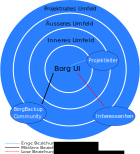
\includegraphics[width=.9\textwidth]{pictures/stakeholder_diagramm.pdf}
\caption{\label{fig:org0f40a2a}
Stakeholder Diagramm}
\end{figure}

\newpage
\begin{landscape}
\begin{table}[htbp]
\centering
\begin{tabular}{|>{\columncolor[HTML]{EFEFEF}}p{0.8cm}|l|l|p{8cm}|l|}
\hline
\textbf{Nr}.\cellcolor[HTML]{C0C0C0} & \textbf{Stakeholder}\cellcolor[HTML]{C0C0C0} & \textbf{Einfluss}\cellcolor[HTML]{C0C0C0} & \textbf{Anforderung/Wünsche}\cellcolor[HTML]{C0C0C0} & \textbf{Wahrscheinlichkeit}\cellcolor[HTML]{C0C0C0}\\
\hline
1. & \gls{borg} Community & gering & - Eine Applikation die den Umfang von \gls{borg} abdeckt & mittel\\
 &  &  & - Open-Source & hoch\\
 &  &  & - Mitsprachrecht bei der Entwicklung & niedrig\\
\hline
2. & User & gering & - Eine einfache Anwendung & hoch\\
 &  &  & - Einmal einrichten und vergessen & mittel\\
\hline
3. & Interessenten & gering & - Einfach verständliches Projekt Repository & hoch\\
 &  &  & - Einfaches Setup zum testen & hoch\\
\hline
4. & Projektleiter & hoch & - Stabile Anwendung erstellen & mittel\\
 &  &  & - Ein nachhaltiges Projekt starten & mittel\\
 &  &  & - Anerkennung im fachlichen Umfeld & niedrig\\
\hline
\end{tabular}
\caption{\label{tab:orgf6b1b5b}
Umweltanalyse}

\end{table}
\end{landscape}

\subsection{Risiko-Analyse}
\label{sec:org892f94d}

Bei der Risiko-Analyse wird von einem durchschnittlichen Benutzer ausgegangen,
der zur Zeit noch keine Backups macht und beginnen möchte \gls{borg} zu nutzen, um
auf einer externen Harddisk seine Backups zu speichern.

Es wird dabei eine Ist/Soll Analyse gemacht, um die Lösung gegenüber der
bestehenden Möglichkeiten zu vergleichen. Jedes Risiko wurde entsprechend der
Tabelle: (\ref{tab:orge1c188d}) nach der Wahrscheinlichkeit des Eintreffens
bewertet und entsprechend der Tabelle: (\ref{tab:org6b71d1b}) nach seiner Auswirkung
im Bezug auf die Nützlichkeit der gemachten Backups.

In der Tabelle: (\ref{tab:org5188bca}) sind dabei die Risiken für das
Szenario aufgelistet und nummeriert. In der Abbildung:(\ref{fig:orgba8df6b}), ist die
Bewertung des Ist-Risikos grafisch dargestellt und in der
Abbildung:(\ref{fig:org214fefa}), ist das Soll-Risiko, welches mit dieser Arbeit
angestrebt wird, ebenfalls grafisch dargestellt.

Es sollte im Rahmen der Arbeit möglich sein die meisten Risiken zu verringern.
Da automatische Hintergrundbackups jedoch nur ein Kann-Ziel sind wir in dieser
Analyse nicht davon ausgegangen das man das Risiko Nr. 5 im Rahmen dieser
Arbeit reduzieren kann.

\begin{table}[H]
\centering
\begin{tabular}{l|l}
\textbf{Bewertung} & \textbf{Beschreibung: Wahrscheinlichkeit (W)}\\
\hline
1 = gering & Unwahrscheinlich, <20\%\\
2 = mittel & Mässig wahrscheinlich, 20-50\%\\
3 = hoch & Hohe Wahrscheinlichkeit > 50\%\\
\end{tabular}
\caption{\label{tab:orge1c188d}
Risikobewertung Wahrscheinlichkeit}

\end{table}

\begin{table}[H]
\centering
\begin{tabular}{l|l}
\textbf{Bewertung} & \textbf{Beschreibung: Auswirkung (A)}\\
\hline
1 = gering & Geringe Auswirkungen auf Nützlichkeit\\
2 = mittel & Mittlere Auswirkung auf die Nützlichkeit\\
3 = hoch & Hohe Auswirkung auf die Nützlichkeit\\
\end{tabular}
\caption{\label{tab:org6b71d1b}
Risikobewertung Auswirkung}

\end{table}

\begin{table}[H]
\centering
\begin{tabular}{|>{\columncolor[HTML]{EFEFEF}}p{0.1\textwidth}|p{0.8\textwidth}|}
\hline
\textbf{Nr.}\cellcolor[HTML]{C0C0C0} & \textbf{Beschreibung}\cellcolor[HTML]{C0C0C0}\\
\hline
1. & Der Benutzer hat noch nie die Kommandozeile verwendet und scheitert bereits an der Installation von \gls{borg}.\\
\hline
2. & Der Benutzer verwendet keine Verschlüsselung und verliert seine Harddisk.\\
\hline
3. & Der Benutzer speichert die Backups auf der internen statt der externen Harddisk.\\
\hline
4. & Der Benutzer löscht aus Versehen ein Backup.\\
\hline
5. & Der Anwender vergisst die Backups zu machen.\\
\hline
\end{tabular}
\caption{\label{tab:org5188bca}
Risikobeschreibung}

\end{table}

\begin{figure}[H]
\centering
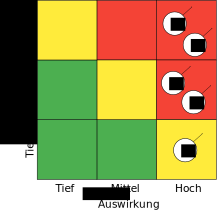
\includegraphics[width=9cm]{pictures/istrisiko.pdf}
\caption{\label{fig:orgba8df6b}
Grafische Darstellung der Ist-Risikoanalyse}
\end{figure}

\begin{figure}[H]
\centering
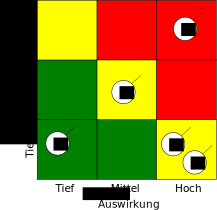
\includegraphics[width=9cm]{pictures/sollrisiko.pdf}
\caption{\label{fig:org214fefa}
Grafische Darstellung der Soll-Risikoanalyse}
\end{figure}

\newpage
\subsection{SWOT-Analyse}
\label{sec:orgcd65a92}

Die SWOT-Analyse ist eine Methode, die Stärken, Schwächen, Chancen und
Gefahren zu erkennen, indem eine 4-Felder-Matrix ausgefüllt wird.

Wichtig vor dem Ausfüllen der SWOT-Analyse ist es, ein klares Ziel zu
haben. Die ausgefüllte SWOT-Analyse für dieses Projekt ist in der
Abbildung:(\ref{fig:orgca071e6}) zu sehen.

\begin{figure}[htbp]
\centering
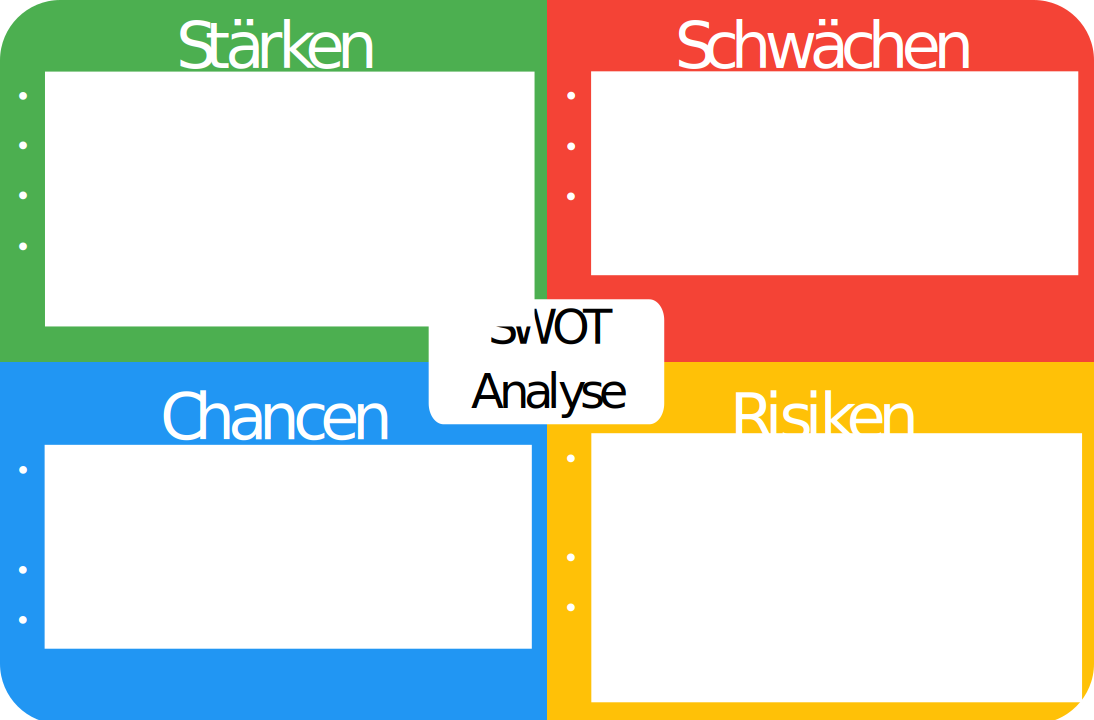
\includegraphics[width=.9\linewidth]{pictures/swot_analyse.pdf}
\caption{\label{fig:orgca071e6}
SWOT Analyse des Projektes}
\end{figure}

\subsection{Anforderungskatalog}
\label{sec:orgc1b2ce7}

Der Anforderungskatalog entspricht 1 zu 1 den Zielen, welche in der Tabelle
\ref{tab:org47ae745} definiert wurden. Im Zeitplan wurde der Fokus hauptsächlich
auf die Muss-Ziele gelegt. Ein paar der Kann-Ziele sind im Konzept jedoch auch
abgebildet.

\subsection{Use Cases}
\label{sec:org4fc4fe3}

Ein Use Case sammelt alle möglichen Szenarien, die eintreten können,
wenn ein Akteur versucht, mithilfe des betrachteten Systems ein
bestimmtes Ziel zu erreichen. Dabei beschreibt er, was beim Versuch der
Zielerreichung passieren kann. Je nach Ablauf kann auch ein Fehlschlag
ein Ergebnis eines Anwendungsfalls sein (e.g. falsches Passwort beim
Login). Dabei wird die technische Lösung nicht konkret beschrieben.
Die Detailstufe kann dabei sehr unterschiedlich sein.\footcite{usecase}

\subsubsection{Anwendungsfalldiagramm}
\label{sec:orgd6378d1}

"`Ein Anwendungsfalldiagramm \ldots{} ist eine der 14 Diagrammarten der
Unified Modelling Language (UML), einer Sprache für die Modellierung
der Strukturen und des Verhaltens von Software- und anderen Systemen.
Es stellt Anwendungsfälle und Akteure mit ihren jeweiligen
Abhängigkeiten und Beziehungen dar."'\footcite{usecasediagramm}

Das Anwendungsfalldiagramm für das \gls{borg} \gls{gui} ist in der Abbildung:
(\ref{fig:org2b532cd}) zu sehen.

\newpage
\begin{landscape}
\begin{figure}[htbp]
\centering
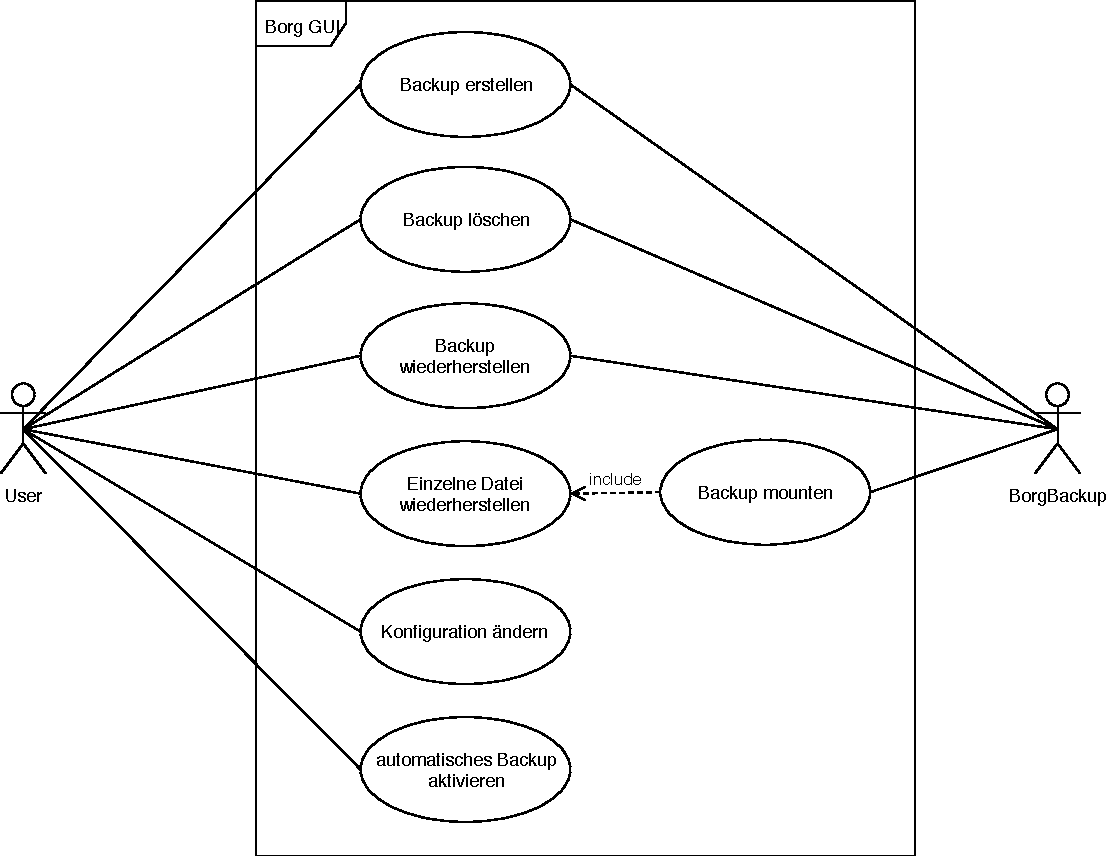
\includegraphics[width=.9\linewidth]{pictures/use_case.pdf}
\caption{\label{fig:org2b532cd}
Anwendungsfalldiagramm}
\end{figure}
\end{landscape}
\newpage

\subsubsection{Use Cases Detailbeschreibung}
\label{sec:org8d11acf}

Use Cases werden in der Regel mithilfe einer sogenannten Use Case Schablone im
Detail beschrieben, damit klar ist, wie der Ablauf jeweils genau aussieht. Die
in diesem Projekt verwendete Schablone wurde von Alistair Cockburn definiert.

Die nachfolgend aufgeführten Use Cases, Tabellen:(\ref{tab:org8002dbd}, \ref{tab:orgbacc4ee},
\ref{tab:org64ae04d}, \ref{tab:orgcd2fced}, \ref{tab:orgee72b48}, \ref{tab:org78c0355}, \ref{tab:org570704b})
wurden dem Anwendungsfalldiagramm, Abbildung:(\ref{fig:org2b532cd}), entnommen und
zusätzlich noch um jeweils ein Aktivitätsdiagramm, Abbildungen:
(\ref{fig:org352c0b4}, \ref{fig:org425e69a}, \ref{fig:org5105e54},
\ref{fig:org64825a2}, \ref{fig:org0683d41}, \ref{fig:org46a3d37}), erweitert
um den Ablauf verständlicher zu machen.

Ein Aktivitätsdiagramm ist dabei ein hilfreiches UML Diagramm zum Erweitern von
Use Cases und zeigt einem gut die Zuständigkeiten der Aktoren auf.

\paragraph{Use Case 1.0 Backup erstellen}
\label{sec:org2fc1bbc}

{\footnotesize
\begin{longtable}{|>{\columncolor[HTML]{EFEFEF}}p{.235\textwidth}|p{.7\textwidth}|}
\hline
\textbf{Identifier + Name} & 1.0 Backup erstellen\\
\hline
\endfirsthead
\multicolumn{2}{l}{Fortsetzung von vorheriger Seite} \\
\hline

\textbf{Identifier + Name} & 1.0 Backup erstellen \\

\hline
\endhead
\hline\multicolumn{2}{r}{Fortsetzung nächste Seite} \\
\endfoot
\endlastfoot
\hline
\textbf{Description} & Das erstellen einer Datensicherung durch \gls{borg} anstossen.\\
\hline
\textbf{Actors} & Benutzer\\
\hline
\textbf{Status} & Freigegeben\\
\hline
\textbf{Includes} & -\\
\hline
\textbf{Trigger} & User möchte ein Backup erstellen.\\
\hline
\textbf{Preconditions} & Die Applikation wurde gestartet.\\
\hline
\textbf{Postconditions} & Das erstellte Backup wird angezeigt.\\
\hline
\textbf{Normal Flow} & 1. Den Quellpfad auswählen.\\
 & 2. Den Button "`Backup"' anklicken.\\
 & 3. Ein Pop mit Fortschrittsbalken erscheint und zeigt die Zeit bis zum Ende des Backups an.\\
 & 4. Am Ende des Backups verschwindet das Pop-up wieder.\\
 & 5. Die Liste der Backups aktualisiert sich.\\
\hline
\textbf{Alternative Flow} & -\\
\hline
\textbf{Notes} & -\\
\hline
\textbf{UC History} & 1.0 Draft erstellt durch AZ\\
\hline
\textbf{Author} & A. Zweili\\
\hline
\textbf{Date} & 30.12.2018\\
\hline
\caption{\label{tab:org8002dbd}
Use Case 1.0 Backup erstellen}
\\
\end{longtable}
}
\begin{figure}[htbp]
\centering
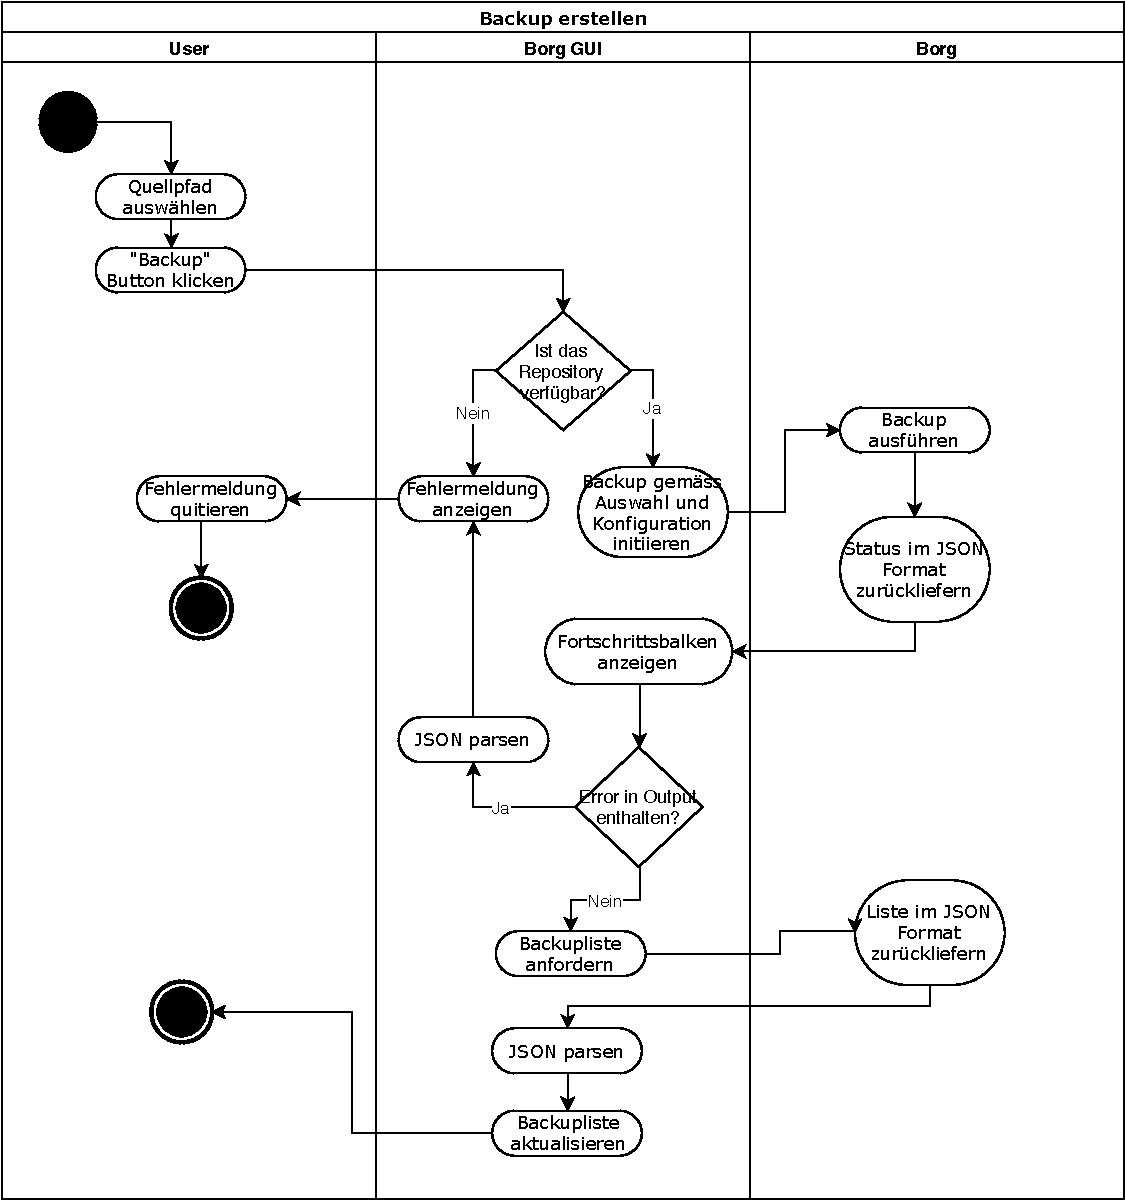
\includegraphics[width=.9\linewidth]{pictures/activity_backup.pdf}
\caption{\label{fig:org352c0b4}
Aktivitätsdiagramm zum Erstellen eines Backups}
\end{figure}
\newpage
\paragraph{Use Case 2.0 Backup löschen}
\label{sec:org3bcf37a}

{\footnotesize
\begin{longtable}{|>{\columncolor[HTML]{EFEFEF}}p{.235\textwidth}|p{.7\textwidth}|}
\hline
\textbf{Identifier + Name} & 2.0 Backup löschen\\
\hline
\endfirsthead
\multicolumn{2}{l}{Fortsetzung von vorheriger Seite} \\
\hline

\textbf{Identifier + Name} & 2.0 Backup löschen \\

\hline
\endhead
\hline\multicolumn{2}{r}{Fortsetzung nächste Seite} \\
\endfoot
\endlastfoot
\hline
\textbf{Description} & Ein zuvor erstelltes Backup wird gelöscht.\\
\hline
\textbf{Actors} & Benutzer\\
\hline
\textbf{Status} & Freigegeben\\
\hline
\textbf{Includes} & -\\
\hline
\textbf{Trigger} & Ein User möchte ein bestehendes Backup löschen.\\
\hline
\textbf{Preconditions} & Use Case 1.0 ausgeführt.\\
\hline
\textbf{Postconditions} & Das gelöschte Backup wird nicht mehr aufgelistet.\\
\hline
\textbf{Normal Flow} & 1. Ein Backup aus der Liste auswählen.\\
 & 2. Den Button "`Delete anklicken"'.\\
 & 3. Ein Bestätigungsdialog erscheint.\\
 & 4. Im Dialog den "`Ok"' Button anklicken.\\
\hline
\textbf{Alternative Flow} & 1. Ein Backup aus der Liste auswählen.\\
 & 2. Den Button "`Delete anklicken"'.\\
 & 3. Ein Bestätigungsdialog erscheint.\\
 & 4. Die Aktion mit einem Klick auf den "`Cancel"' Button abbrechen.\\
\hline
\textbf{Notes} & -\\
\hline
\textbf{UC History} & 1.0 Draft erstellt durch AZ\\
\hline
\textbf{Author} & A. Zweili\\
\hline
\textbf{Date} & 30.12.2018\\
\hline
\caption{\label{tab:orgbacc4ee}
Use Case 2.0 Backup löschen}
\\
\end{longtable}
}
\begin{figure}[htbp]
\centering
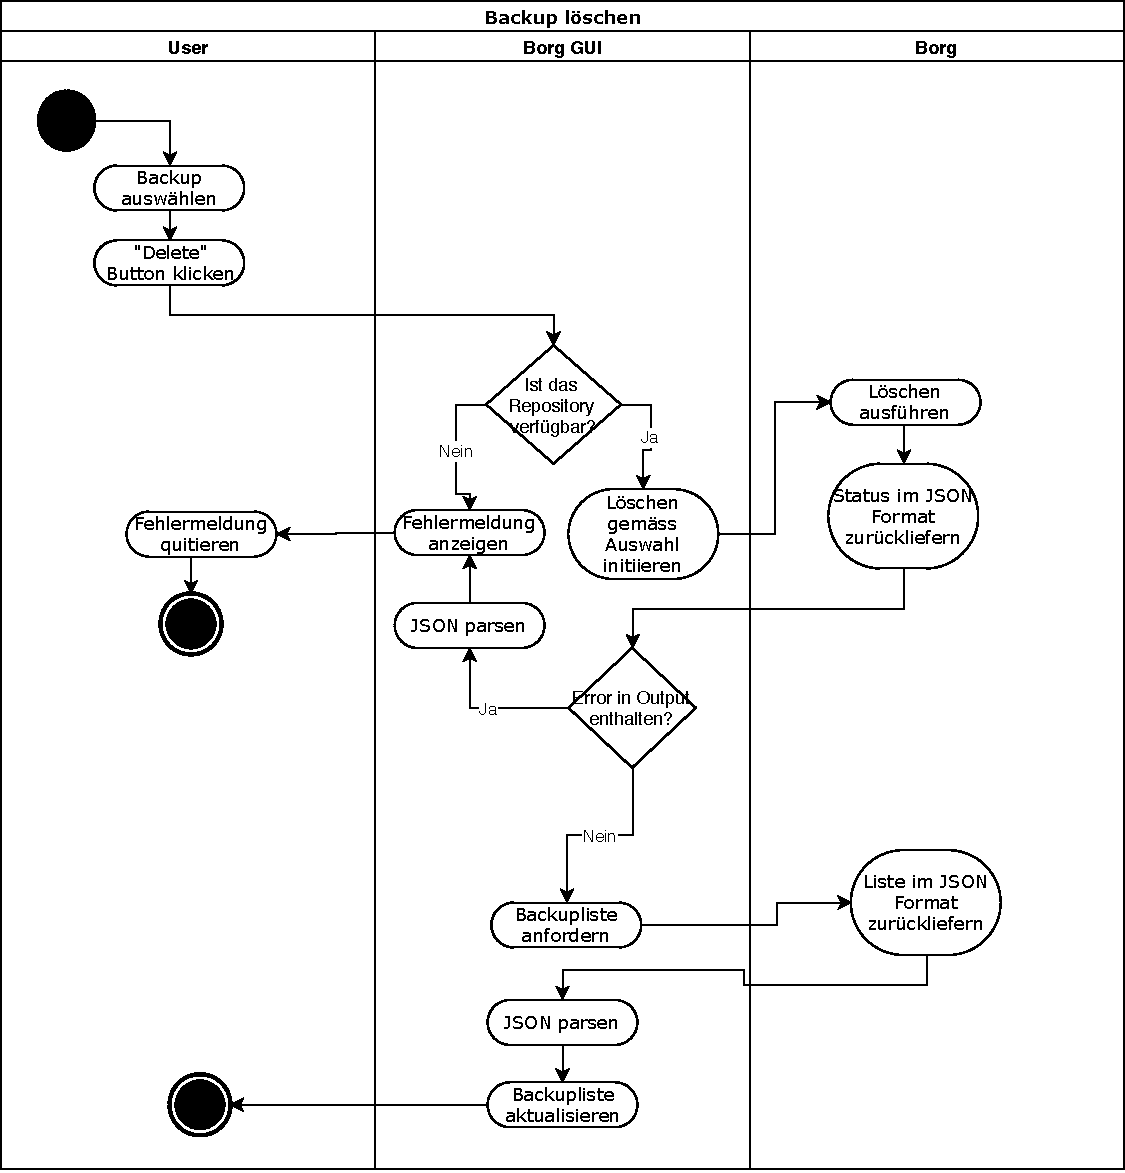
\includegraphics[width=.9\linewidth]{pictures/activity_delete.pdf}
\caption{\label{fig:org425e69a}
Aktivitätsdiagramm zum Löschen eines Backups}
\end{figure}
\newpage
\paragraph{Use Case 3.0 Backup wiederherstellen}
\label{sec:org5b0073b}

{\footnotesize
\begin{longtable}{|>{\columncolor[HTML]{EFEFEF}}p{.235\textwidth}|p{.7\textwidth}|}
\hline
\textbf{Identifier + Name} & 3.0 Backup wiederherstellen\\
\hline
\endfirsthead
\multicolumn{2}{l}{Fortsetzung von vorheriger Seite} \\
\hline

\textbf{Identifier + Name} & 3.0 Backup wiederherstellen \\

\hline
\endhead
\hline\multicolumn{2}{r}{Fortsetzung nächste Seite} \\
\endfoot
\endlastfoot
\hline
\textbf{Description} & Alle Dateien eines Backups wiederherstellen.\\
\hline
\textbf{Actors} & User\\
\hline
\textbf{Status} & Freigegeben\\
\hline
\textbf{Includes} & -\\
\hline
\textbf{Trigger} & Daten sollen wieder hergestellt werden.\\
\hline
\textbf{Preconditions} & Use Case 1.0 wurde ausgeführt.\\
\hline
\textbf{Postconditions} & Die Dateien aus dem Backup wurde im angegeben Pfad wiederhergestellt.\\
\hline
\textbf{Normal Flow} & 1. Ein Backup aus der Liste auswählen.\\
 & 2. Den Button "`Restore"' klicken.\\
 & 3. Ein Pop-up zur Auswahl eines Zielpfades erscheint.\\
 & 4. Den Zielpfad mit klick auf "`Choose"' bestätigen.\\
 & 5. Ein Dateiexplorer öffnet sich mit dem ausgewählt Pfad und enthält die Dateien aus dem Backup.\\
\hline
\textbf{Alternative Flow} & 1. Ein Backup aus der Liste auswählen.\\
 & 2. Den Button "`Restore"' klicken.\\
 & 3. Ein Pop-up zur Auswahl eines Zielpfades erscheint.\\
 & 4. Die Aktion mit klick auf "`Cancel"' abbrechen.\\
\hline
\textbf{Notes} & -\\
\hline
\textbf{UC History} & 1.0 Draft erstellt durch AZ\\
\hline
\textbf{Author} & A. Zweili\\
\hline
\textbf{Date} & 30.12.2018\\
\hline
\caption{\label{tab:org64ae04d}
Use Case 3.0 Backup wiederherstellen}
\\
\end{longtable}
}

\begin{figure}[htbp]
\centering
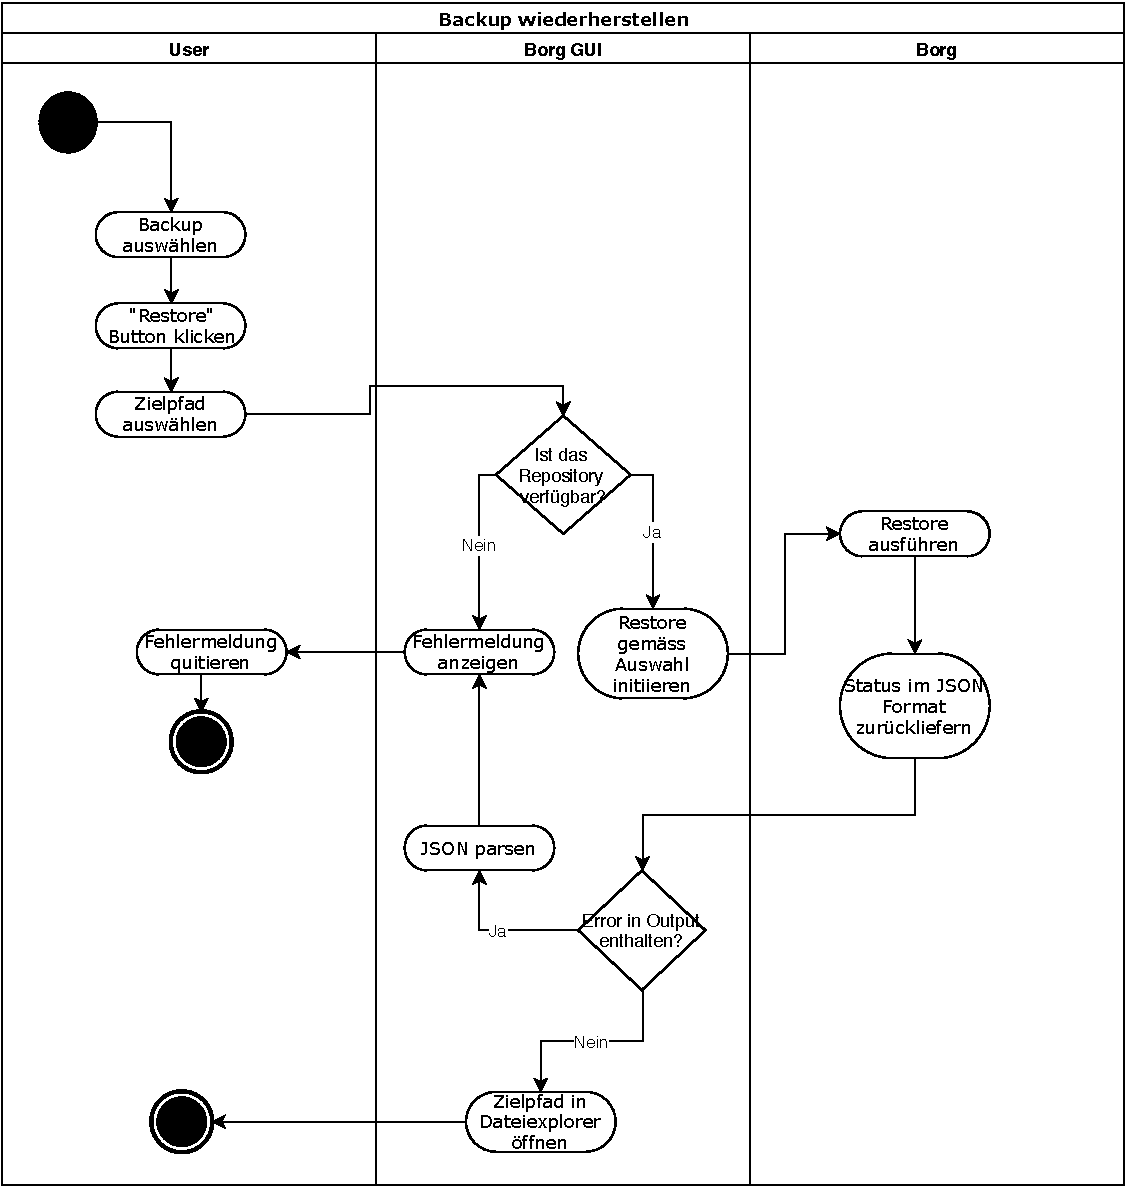
\includegraphics[width=.9\linewidth]{pictures/activity_restore.pdf}
\caption{\label{fig:org5105e54}
Aktivitätsdiagramm zum Wiederherstellen eines Backups}
\end{figure}
\newpage
\paragraph{Use Case 4.0 Einzelne Datei wiederherstellen}
\label{sec:orge029c6d}

{\footnotesize
\begin{longtable}{|>{\columncolor[HTML]{EFEFEF}}p{.235\textwidth}|p{.7\textwidth}|}
\hline
\textbf{Identifier + Name} & 4.0 Einzelne Datei wiederherstellen\\
\hline
\endfirsthead
\multicolumn{2}{l}{Fortsetzung von vorheriger Seite} \\
\hline

\textbf{Identifier + Name} & 4.0 Einzelne Datei wiederherstellen \\

\hline
\endhead
\hline\multicolumn{2}{r}{Fortsetzung nächste Seite} \\
\endfoot
\endlastfoot
\hline
\textbf{Description} & Das spezifische Wiederherstellen von einer oder mehreren Dateien.\\
\hline
\textbf{Actors} & User\\
\hline
\textbf{Status} & Freigegeben\\
\hline
\textbf{Includes} & Use Case 4.1\\
\hline
\textbf{Trigger} & Daten sollen wieder hergestellt werden.\\
\hline
\textbf{Preconditions} & Use Case 1.0 wurde ausgeführt.\\
\hline
\textbf{Postconditions} & -\\
\hline
\textbf{Normal Flow} & 1. Ein Backup aus der Liste auswählen.\\
 & 2. Auf den Button "`Mount"' klicken.\\
 & 3. Use Case 4.1 wird ausgeführt.\\
 & 4. Ein Dateiexplorer öffnet sich mit dem ausgewählt Pfad und enthält die Dateien aus dem Backup.\\
 & 5. Wird die Applikation geschlossen wird das Backup ausgehängt.\\
\hline
\textbf{Alternative Flow} & -\\
\hline
\textbf{Notes} & -\\
\hline
\textbf{UC History} & 1.0 Draft erstellt durch AZ\\
\hline
\textbf{Author} & A. Zweili\\
\hline
\textbf{Date} & 30.12.2018\\
\hline
\caption{\label{tab:orgcd2fced}
Use Case 4.0 Einzelne Datei wiederherstellen}
\\
\end{longtable}
}

\begin{figure}[htbp]
\centering
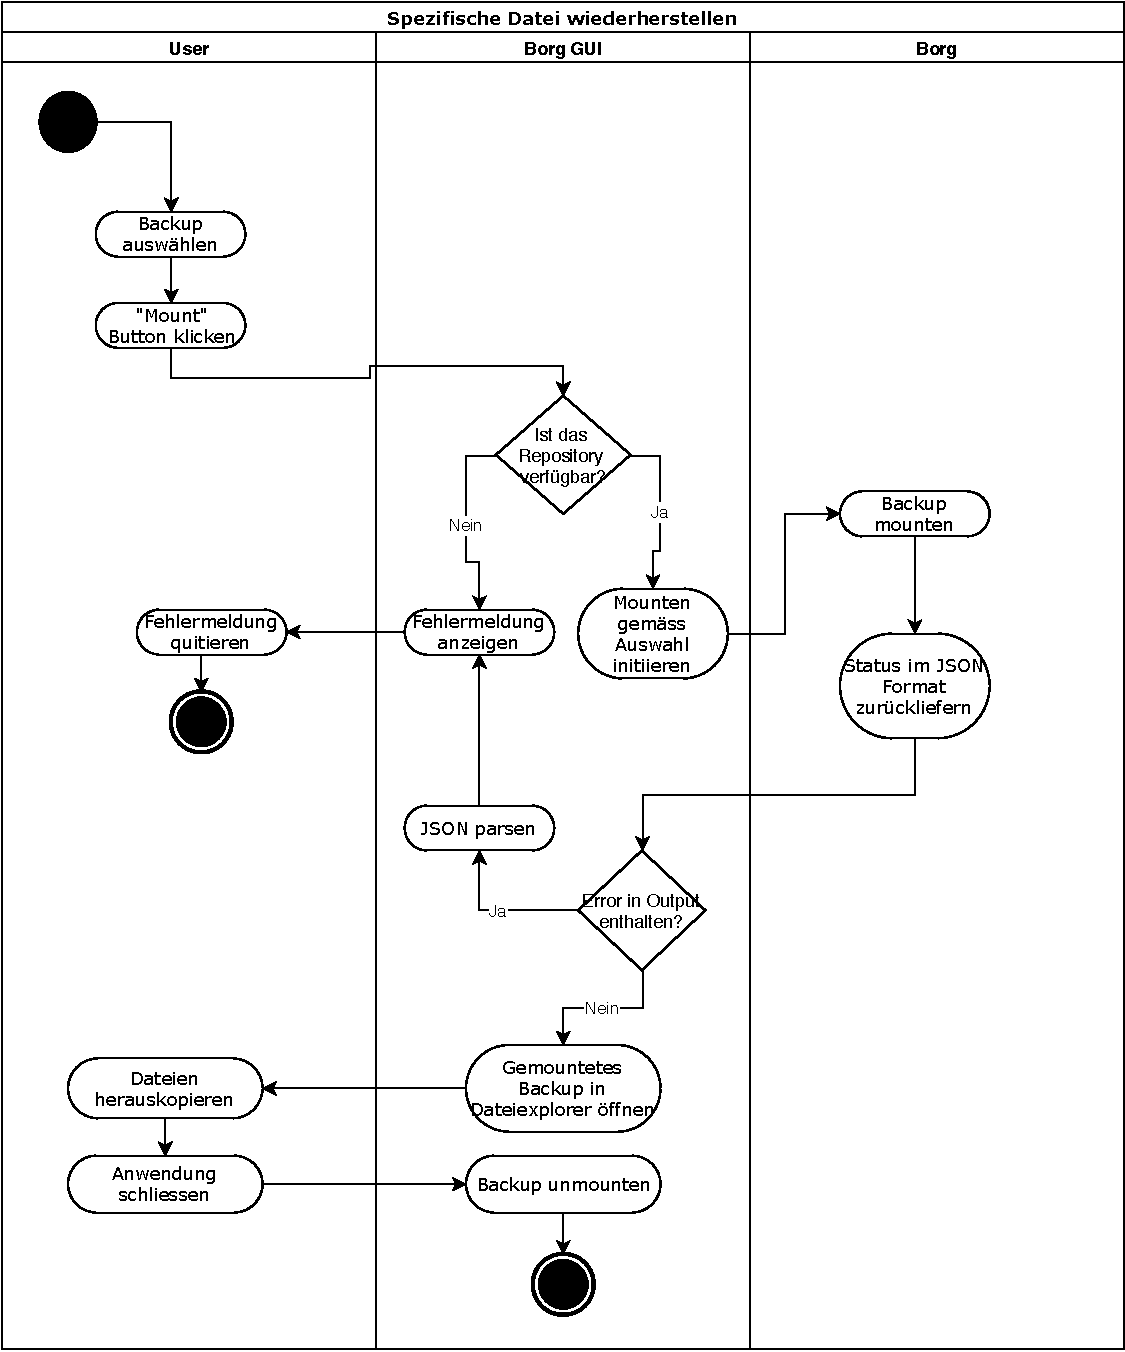
\includegraphics[width=.9\linewidth]{pictures/activity_mount.pdf}
\caption{\label{fig:org64825a2}
Aktivitätsdiagramm für das spezifische Wiederherstellen einer Datei}
\end{figure}
\newpage
\paragraph{Use Case 4.1 Backup mounten}
\label{sec:orgb7e9d21}

{\footnotesize
\begin{longtable}{|>{\columncolor[HTML]{EFEFEF}}p{.235\textwidth}|p{.7\textwidth}|}
\hline
\textbf{Identifier + Name} & 4.1 Backup mounten\\
\hline
\endfirsthead
\multicolumn{2}{l}{Fortsetzung von vorheriger Seite} \\
\hline

\textbf{Identifier + Name} & 4.1 Backup mounten \\

\hline
\endhead
\hline\multicolumn{2}{r}{Fortsetzung nächste Seite} \\
\endfoot
\endlastfoot
\hline
\textbf{Description} & Ein Backup wird als FUSE gemountet.\\
\hline
\textbf{Actors} & Borg GUI, \gls{borg}\\
\hline
\textbf{Status} & Freigegeben\\
\hline
\textbf{Includes} & -\\
\hline
\textbf{Trigger} & Das Borg GUI gibt an \gls{borg} den Input zum mounten weiter.\\
\hline
\textbf{Preconditions} & Use Case 1.0 wurde ausgeführt.\\
\hline
\textbf{Postconditions} & Das Backup wurde gemountet.\\
\hline
\textbf{Normal Flow} & 1. Borg GUI sammelt die Backup ID in Use Case 4.0.\\
 & 2. Borg GUI übergibt die Backup ID an \gls{borg} zusammen mit einem Zielpfad.\\
 & 3. \gls{borg} hängt das Backup als FUSE Laufwerk am Zielpfad ein.\\
 & 4. \gls{borg} meldet Erfolg an Borg GUI.\\
\hline
\textbf{Alternative Flow} & 1. Borg GUI sammelt die Backup ID in Use Case 4.0.\\
 & 2. Borg GUI übergibt die Backup ID an \gls{borg} zusammen mit einem Zielpfad.\\
 & 3. \gls{borg} hängt das Backup als FUSE Laufwerk am Zielpfad ein.\\
 & 4. \gls{borg} meldet einen Fehler an Borg GUI.\\
\hline
\textbf{Notes} & -\\
\hline
\textbf{UC History} & 1.0 Draft erstellt durch AZ\\
\hline
\textbf{Author} & A. Zweili\\
\hline
\textbf{Date} & 30.12.2018\\
\hline
\caption{\label{tab:orgee72b48}
Use Case 4.1 Backup mounten}
\\
\end{longtable}
}

\newpage
\paragraph{Use Case 5.0 Konfiguration ändern}
\label{sec:org202b2c5}

{\footnotesize
\begin{longtable}{|>{\columncolor[HTML]{EFEFEF}}p{.235\textwidth}|p{.7\textwidth}|}
\hline
\textbf{Identifier + Name} & 5.0 Konfiguration ändern\\
\hline
\endfirsthead
\multicolumn{2}{l}{Fortsetzung von vorheriger Seite} \\
\hline

\textbf{Identifier + Name} & 5.0 Konfiguration ändern \\

\hline
\endhead
\hline\multicolumn{2}{r}{Fortsetzung nächste Seite} \\
\endfoot
\endlastfoot
\hline
\textbf{Description} & Das Verändern und Speichern der Konfiguration der Applikation.\\
\hline
\textbf{Actors} & User\\
\hline
\textbf{Status} & Freigegeben\\
\hline
\textbf{Includes} & -\\
\hline
\textbf{Trigger} & Ein User möchte die Einstellungen der Applikation anpassen.\\
\hline
\textbf{Preconditions} & Applikation gestartet.\\
\hline
\textbf{Postconditions} & -\\
\hline
\textbf{Normal Flow} & 1. Auf den Button "`Settings"' klicken.\\
 & 2. Ein neues Fenster mit den Einstellungen öffnet sich.\\
 & 3. Der Benutzer ändert mindestens eine Einstellung.\\
 & 4. Der Button "`OK"' wird angeklickt.\\
 & 5. Die Konfiguration wird in die Konfigurationsdatei geschrieben und in der Applikation geladen.\\
\hline
\textbf{Alternative Flow} & 1. Auf den Button "`Settings"' klicken.\\
 & 2. Ein neues Fenster mit den Einstellungen öffnet sich.\\
 & 3. Der Benutzer kann Einstellungen ändern.\\
 & 4. Der Button "`Cancel"' wird angeklickt.\\
 & 5. Jegliche Änderungen werden verworfen und die Konfigurationsdatei bleibt im aktuellen Zustand.\\
\hline
\textbf{Notes} & -\\
\hline
\textbf{UC History} & 1.0 Draft erstellt durch AZ\\
\hline
\textbf{Author} & A. Zweili\\
\hline
\textbf{Date} & 30.12.2018\\
\hline
\caption{\label{tab:org78c0355}
Use Case 5.0 Konfiguration ändern}
\\
\end{longtable}
}

\begin{figure}[htbp]
\centering
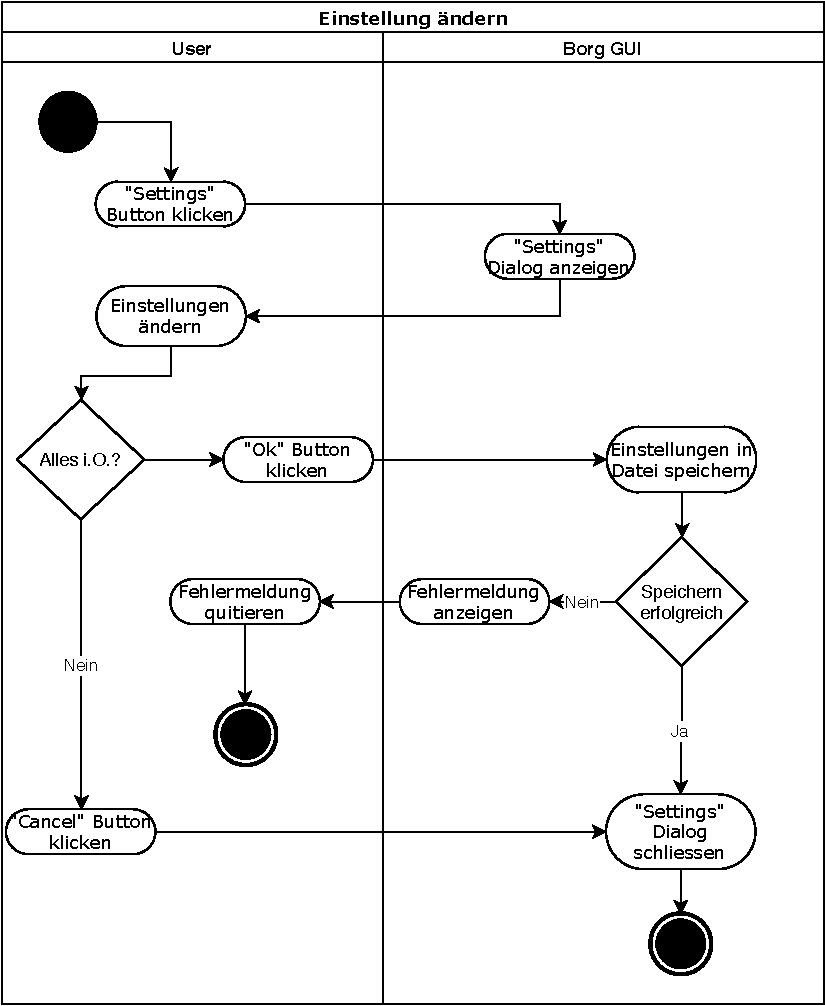
\includegraphics[width=.9\linewidth]{pictures/activity_settings.pdf}
\caption{\label{fig:org0683d41}
Aktivitätsdiagramm zum Ändern von Einstellungen}
\end{figure}
\newpage
\paragraph{Use Case 6.0 automatische Backups aktivieren}
\label{sec:org76066d8}

{\footnotesize
\begin{longtable}{|>{\columncolor[HTML]{EFEFEF}}p{.235\textwidth}|p{.7\textwidth}|}
\hline
\textbf{Identifier + Name} & 6.0 automatische Backups aktivieren\\
\hline
\endfirsthead
\multicolumn{2}{l}{Fortsetzung von vorheriger Seite} \\
\hline

\textbf{Identifier + Name} & 6.0 automatische Backups aktivieren \\

\hline
\endhead
\hline\multicolumn{2}{r}{Fortsetzung nächste Seite} \\
\endfoot
\endlastfoot
\hline
\textbf{Description} & Ein Systemdienst wird hinterlegt zum ausführen automatischer Backups.\\
\hline
\textbf{Actors} & User\\
\hline
\textbf{Status} & Freigegeben\\
\hline
\textbf{Includes} & -\\
\hline
\textbf{Trigger} & Ein User möchte automatisierte Backups haben.\\
\hline
\textbf{Preconditions} & Eine funktionierende Konfiguration muss hinterlegt sein.\\
 & Applikation gestartet.\\
\hline
\textbf{Postconditions} & Ein Systemdienst wurde erstellt welcher jeden Tag ein Backup macht.\\
\hline
\textbf{Normal Flow} & 1. Auf den Button "`Settings"' klicken.\\
 & 2. Bei der Option "`Automatic Backups"' den Hacken setzen.\\
 & 3. Die Settings mit klick auf "`Ok"' schliessen und speichern.\\
\hline
\textbf{Alternative Flow} & 1. Auf den Button "`Settings"' klicken.\\
 & 2. Bei der Option "`Automatic Backups"' den Hacken setzen.\\
 & 3. Die Aktion mit klick auf "`Cancel"' abbrechen\\
\hline
\textbf{Notes} & -\\
\hline
\textbf{UC History} & 1.0 Draft erstellt durch AZ\\
\hline
\textbf{Author} & A. Zweili\\
\hline
\textbf{Date} & 30.12.2018\\
\hline
\caption{\label{tab:org570704b}
Use Case 6.0 automatische Backups aktivieren}
\\
\end{longtable}
}

\begin{figure}[htbp]
\centering
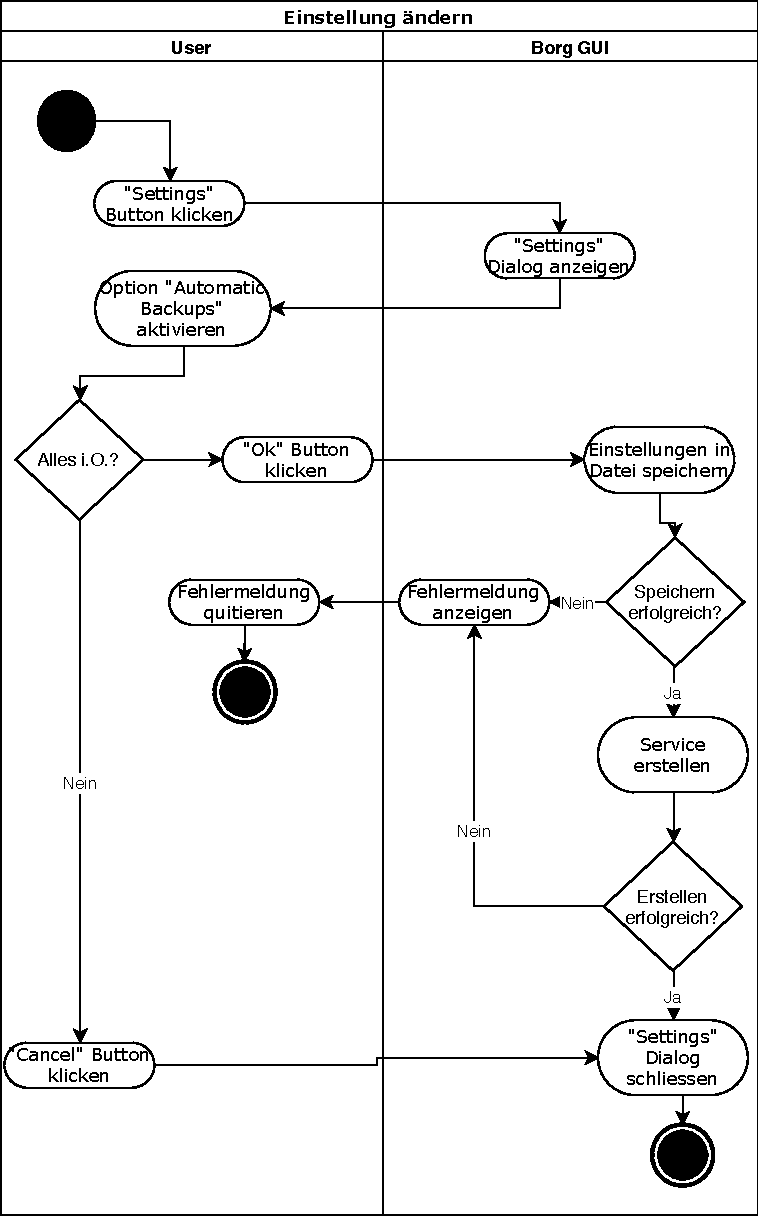
\includegraphics[width=.9\linewidth]{pictures/activity_automatic.pdf}
\caption{\label{fig:org46a3d37}
Aktivitätsdiagramm zum Aktivieren von automatischen Backups}
\end{figure}
\newpage
\section{Konzept}
\label{sec:org5d9b432}

\subsection{Varianten}
\label{sec:orgf462e72}

Da Borg eine \gls{json} API zur Verfügung stellt gibt es diverse Möglichkeiten, um
das Programm anzubinden. Da das Ziel ist, das Programm normalen Nutzern
zugänglicher zu machen, bietet sich ein normales Desktop Programm am ehesten
an. Desktop Programme werden von allen Computer Usern täglich genutzt und sind
somit etwas was sie kennen. Zudem ist es für die User auch viel einfacher zu
verstehen als sie vor der Nutzung einen lokalen Webserver starten müssten und
diesen im Anschluss zur Nutzung wieder beenden müssten.

\subsubsection{Bewertung}
\label{sec:org5bc7aa3}

Mit der Idee aus der Einleitung zu den Varianten wurde dann eine Tabelle, mit
Anforderungen an die Technologien, erstellt. Die Bewertungspunkte setzen sich
einerseits aus Projektzielen anderseits aus für das Projekt sinnvollen Punkten
zusammen. Dadurch ergeben sich dann die Bewertungen, welche in der
Tabelle:(\ref{tab:orgb2f6278}) aufgenommen wurden. Die möglichen Varianten wurden danach
bewertet. Die effektive Berechnung des Resultats wird nach folgender Formel
durchgeführt.

\begin{equation}
G * EP = KE
\end{equation}

Also die Gewichtung(\emph{G}) multipliziert mit der erreichten Punktzahl(\emph{EP})
ergibt das Kriteriumsergebnis(\emph{KE}). Für das Endresultat wird dann die Summe
über alle Kriterien gebildet. Die Variante mit der höchsten Summe wurde für das
Projekt ausgewählt.

Mussziele erhalten dabei eine
Gewichtung von 10 und Wunschziele eine Gewichtung entsprechend der Bewertung in
der Tabelle Projektziele (\ref{tab:org47ae745}).

\begin{table}[htbp]
\centering
\begin{tabular}{|>{\columncolor[HTML]{EFEFEF}}p{4cm}|c|p{2cm}|p{2cm}|p{2cm}|}
\hline
\textbf{Kriterium}\cellcolor[HTML]{C0C0C0} & \textbf{Gewichtung}\cellcolor[HTML]{C0C0C0} & \textbf{max. Punktzahl}\cellcolor[HTML]{C0C0C0} & \textbf{erreichte Punktzahl}\cellcolor[HTML]{C0C0C0} & \textbf{Kriteriums- ergebnis}\cellcolor[HTML]{C0C0C0}\\
\hline
1. Cross Plattform nutzbar & 10 & 10 & 10 & 100\\
2. Freie Software & 5 & 10 & 10 & 50\\
3. Vorkenntnisse & 5 & 10 & 10 & 50\\
4. Integriert sich gut ins System & 5 & 10 & 10 & 50\\
5. Ohne spezielle Tools nutzbar & 5 & 10 & 10 & 50\\
6. Lesbarkeit des Codes & 5 & 5 & 5 & 25\\
7. Einfachheit des Setups & 5 & 5 & 5 & 25\\
8. Lernfaktor & 5 & 5 & 5 & 25\\
9. Verbreitung bei der \gls{borg} Community & 5 & 5 & 5 & 25\\
10. Geschwindigkeit der Entwicklung & 3 & 5 & 5 & 15\\
\hline
\textbf{Total} &  &  &  & 415\\
\hline
\end{tabular}
\caption{\label{tab:orgb2f6278}
Muster Bewertungstabelle}

\end{table}

\subsubsection{Backend}
\label{sec:orgb5cc8f9}

Fürs Backend bieten sich die folgende drei Sprachen an: \hyperref[sec:orgb5bf065]{C\#}, \hyperref[sec:orged93496]{C++}, \hyperref[sec:org7f7b6f4]{Python}.
Dies vor allem, weil alle Allrounder Sprachen sind und sich gut für Desktop
Applikationen eignen.

\paragraph{C\#}
\label{sec:orgb5bf065}

C\# ist eine von Microsoft entwickelte Programmiersprache welche viele
Frameworks zur Verfügung hat. Insbesondere aufgrund der grossen kommerziellen
Nutzung und der guten Integration mit Windows hat C\# eine relative grosse
Verbreitung. Bei Linux und OS X ist es jedoch schwieriger C\# zu integrieren und
zu nutzen.

Sie ist zu Teilen \gls{libre}. Die Common Language Runtime, welche für das
Ausführen von Software zuständig ist, ist unter der MIT Lizenz lizenziert
\footcite{csharp} der aktuelle Compiler Roslyn ist unter der Apache Lizenz
verfügbar \footcite{roslyn}. Da es sehr viele offizielle Teile um die Sprache C\#
gibt, kann im Rahmen des Projektes nicht direkt abgeschätzt werden, ob alle
benötigten Teile \gls{libre} sind. Für die Bewertung wird deshalb ein kleinerer
Wert als bei C++ und Python genommen.

C\# ist die Programmiersprache, welche an der IBZ hauptsächlich gelehrt wird.
Dadurch sind die Kenntnisse der Sprache und ihrer Anwendung bereits
einigermassen vorhanden. Ausserhalb der Schule wurde die Sprache jedoch noch nie
eingesetzt.

Entwickelt wird C\# hauptsächlich mit der \gls{ide} Microsoft Visual Studio.
Eine sehr umfangreiche und komplexe Software. Visual Studio ist dabei nur für
Windows und OS X erhältlich. Es ist auch möglich C\# Projekte ausserhalb von
Visual Studio zu erstellen, es ist jedoch nicht sehr einfach.

Der Code ist gut lesbar und es gibt offizielle Styleguides von Microsoft was
den Code über Projekte hinaus einigermassen einheitlich aussehen lässt. Zudem
hilft hier auch Visual Studio stark den Code entsprechend zu formatieren.
Besonders angenehm sind die Klassen- und Methodennamen der offiziellen
Frameworks. Insgesamt sehr gut gelöst aber in Sachen Lesbarkeit noch etwas
hinter Python.

Unter Windows ist das Setup von C\# relativ einfach. Allerdings ist es auch dort
im Vergleich zu Python eine umfangreiche Angelegenheit Visual Studio sauber zu
installieren und nutzbar zu machen. Auf anderen Plattform wird dies leider
nicht einfacher und unter Linux ist es bereits schwierig eine funktionierende
Umgebung in Gang zu bringen.

Da C\# bereits an der IBZ gelernt wird, ist der Lernfaktor hier im Vergleich zu
den anderen Sprachen sicher am kleinsten. Allerdings gibt es noch keinerlei
Kenntnisse beim Einbinden eines der unten aufgeführten \gls{gui} Frameworks.
Daher gibt es auf jeden Fall noch genügend zu lernen.

Die \gls{borg} Community hat vor relativ kurzer Zeit die offizielle Unterstützung
von Windows zurückgezogen. Da C\# eine sehr Windows lastige Sprache ist, wird
daher davon ausgegangen das die Sprache innerhalb der \gls{borg} Community nicht
sehr verbreitet ist.

C\# ist eine stark typisiert Sprache und kompilierte Sprache. Des Weiteren ist
Visual Studio der Erfahrung nach nicht die schnellste Software. Dies alles
führt dazu das C\# nicht gerade die schnellste Sprache zum Programmieren ist.
Jedoch aufgrund des moderneren Unterbaus sicher schneller als C++.

\begin{table}[htbp]
\centering
\begin{tabular}{|>{\columncolor[HTML]{EFEFEF}}p{4cm}|c|p{2cm}|p{2cm}|p{2cm}|}
\hline
\textbf{Kriterium}\cellcolor[HTML]{C0C0C0} & \textbf{Gewichtung}\cellcolor[HTML]{C0C0C0} & \textbf{max. Punktzahl}\cellcolor[HTML]{C0C0C0} & \textbf{erreichte Punktzahl}\cellcolor[HTML]{C0C0C0} & \textbf{Kriteriums- ergebnis}\cellcolor[HTML]{C0C0C0}\\
\hline
1. Cross Plattform nutzbar & 10 & 10 & 8 & 80\\
2. Freie Software & 5 & 10 & 8 & 40\\
3. Vorkenntnisse & 5 & 10 & 6 & 30\\
4. Integriert sich gut ins System & 5 & 10 & 8 & 40\\
5. Ohne spezielle Tools nutzbar & 5 & 10 & 6 & 30\\
6. Lesbarkeit des Codes & 5 & 5 & 4 & 20\\
7. Einfachheit des Setups & 5 & 5 & 2 & 10\\
8. Lernfaktor & 5 & 5 & 3 & 15\\
9. Verbreitung bei der \gls{borg} Community & 5 & 5 & 1 & 5\\
10. Geschwindigkeit der Entwicklung & 3 & 5 & 3 & 9\\
\hline
\textbf{Total} &  &  &  & 279\\
\hline
\end{tabular}
\caption{\label{tab:orga52a741}
C\# Bewertungstabelle}

\end{table}

\paragraph{C++}
\label{sec:orged93496}

C++ ist eine stark typisierte und kompilierte Programmiersprache. Sie ist seit
1998 Teil des ISO Standards \footcite{cpp98}. ISO/IEC 14882:2017 \footcite{cpp17}
ist zurzeit die aktuellste Variante. Die Sprache existiert seit ca. 33 Jahren
und hat eine weitreichende Verbreitung gefunden. C++ ist auf allen
Betriebssystemen gut unterstützt muss jedoch für jedes System separat
kompiliert werden.

Von C++ sind innerhalb des Projektes keinerlei Vorkenntnisse vorhanden. Dies
ist ein sehr hoher Risikofaktor.

C++ kompiliert direkt zu Maschinensprache und ist dadurch sehr performant und
läuft sehr gut auf jedem System. C++ ist im Vergleich zu modernen Sprachen
jedoch relativ komplex und bietet diverse Stolpersteine für Programmierer.

Zum Entwickeln braucht es verhältnismässig wenig. Da die Sprache bereits sehr
alt ist, stammt sie noch aus einer Zeit wo man noch etwas rudimentärer
programmierte. Allerdings braucht man in jedem Fall einen \gls{compiler} um ein
ausführbares Programm zu erzeugen. Bei komplexeren Programmen wird man um
mindestens so etwas wie \glspl{makefile} auch nicht herumkommen

Im Vergleich zu Python oder C\# ist C++ wohl die am schwersten lesbare Sprache.
Zudem gibt es auch keinen zentralen Styleguide, welcher einem vorgeben würde wie
der Code am besten ausschauen sollte. Somit haben sich über die Jahre mehrere
Standards etabliert.

Der Lernfaktor wäre aufgrund der mangelnden Vorkenntnisse hier ganz klar am
Grössten.

Da C++ eine alte Sprache ist geniesst sie auch eine dementsprechende
Verbreitung. Daher ist anzunehmen das sicher mindestens ein grössere Teil der
älteren \gls{borg} Entwickler C++ oder C gelernt haben.

Da C++ auch heute noch zu den meistgenutzten Sprachen gehört gibt es
entsprechend viele Ressourcen dazu und Beispiel Projekte, von denen man ableiten
kann. Auch hilfreiche Libraries gibt es sehr viele, welche den Programmierer
unterstützen können. Die Sprache selber ist jedoch eher umständlich zu
schreiben. Hinzu kommt noch das man, während der Entwicklung immer wieder den
Code kompilieren muss. In einem Projekt mit dieser begrenzten Zeitspanne eher
ungeeignet.

\begin{table}[htbp]
\centering
\begin{tabular}{|>{\columncolor[HTML]{EFEFEF}}p{4cm}|c|p{2cm}|p{2cm}|p{2cm}|}
\hline
\textbf{Kriterium}\cellcolor[HTML]{C0C0C0} & \textbf{Gewichtung}\cellcolor[HTML]{C0C0C0} & \textbf{max. Punktzahl}\cellcolor[HTML]{C0C0C0} & \textbf{erreichte Punktzahl}\cellcolor[HTML]{C0C0C0} & \textbf{Kriteriums- -ergebnis}\cellcolor[HTML]{C0C0C0}\\
\hline
1. Cross Plattform nutzbar & 10 & 10 & 8 & 80\\
2. Freie Software & 5 & 10 & 10 & 50\\
3. Vorkenntnisse & 5 & 10 & 0 & 0\\
4. Integriert sich gut ins System & 5 & 10 & 8 & 40\\
5. Ohne spezielle Tools nutzbar & 5 & 10 & 6 & 30\\
6. Lesbarkeit des Codes & 5 & 5 & 2 & 10\\
7. Einfachheit des Setups & 5 & 5 & 3 & 15\\
8. Lernfaktor & 5 & 5 & 5 & 25\\
9. Verbreitung bei der \gls{borg} Community & 5 & 5 & 3 & 15\\
10. Geschwindigkeit der Entwicklung & 3 & 5 & 2 & 6\\
\hline
\textbf{Total} &  &  &  & 271\\
\hline
\end{tabular}
\caption{\label{tab:orga701895}
C++ Bewertungstabelle}

\end{table}

\newpage
\paragraph{Python}
\label{sec:org7f7b6f4}

Der Python Interpreter ist für eine Vielzahl an Betriebssystemen erhältlich,
inklusive Windows, OS X und Linux. Nahezu jedes Desktop Linux System kommt mit
Python vor installiert. Auch OS X kommt bereits ab Werk mit Python Version 2.
Version 3 lässt sich sehr einfach nachinstallieren und ist einfach nutzbar.
Unter Windows gestaltetet sich die Installation etwas aufwendiger aber auch
nicht sehr kompliziert. Python integriert sich in Windows jedoch etwas weniger
elegant als C\#.

Python ist freie Software unter der Python Software Foundation License
\footcite{python} und wird durch die Python Software Foundation in einem
Community basierten Modell entwickelt.

Die Vorkenntnisse sind im Vergleich zu C++ relativ gross und zu C\# etwas
weniger ausgeprägt. Es wurden damit im Rahmen der Ausbildung schon ein
grösseres Projekt realisiert und ansonsten mehrere kleine Projekte im Privaten
erstellen.

Für Python gibt es ein paar \glspl{ide} welchen den Programmierer bei seiner
Arbeit unterstützen können. Keine davon ist allerdings ein Muss um Python
programmieren zu können. Im einfachsten Fall wäre dies mit Notepad möglich. Ein
Editor mit etwas fortgeschritteneren Features wäre jedoch empfehlenswert.

Python unterstützt mehrere Programmierungsparadigmen wie etwa
objektorientiert, funktionale oder Prozedurale Paradigmen. Bei der Entwicklung
von Python wurde sehr grossen Wert auf die Lesbarkeit der Sprache gelegt. Dies
mit dem Hintergedanken das eine Programmiersprache viel häufiger gelesen als
effektiv geschrieben wird \footcite{pep8}.

Um ein Python Programm zu starten braucht es eigentlich kein grosses Setup.
Solange die Abhängigkeiten vorhanden sind, kann man ein Skript mit einem
einfachen Befehl, Code Snippet (\ref{org3aa94ac}) starten.

\lstset{language=bash,label=org3aa94ac,caption={Minimal Python Setup},captionpos=b,numbers=none}
\begin{sexylisting}{Minimal Python Setup}
python3 example.py
\end{sexylisting}

Da Python schon eine etwas bekanntere Sprache ist, ist der Lernfaktor der
Sprache selber nicht mehr so hoch. Allerdings gibt es noch viele interessante
Konzepte, die man im Zusammenhang mit der Sprache lernen kann. Wie etwa zum
Beispiel multiple Vererbung von Klassen.

\gls{borg} selber wurde in Python geschrieben. Daher ist davon auszugehen das
Python innerhalb dieser Community eine sehr hohe Verbreitung geniesst.

Python ist eine dynamisch typisierte und interpretierte Sprache. Dies bedeutet
das man bei Variablen nicht explizit den Typ angeben muss und die Programme zur
Laufzeit für den Computer übersetzt werden. Interpretierte Sprachen haben den
Vorteil das man mit ihnen in der Regel sehr schnell und unkompliziert
entwickeln kann, dies jedoch zulasten der Performance.

\begin{table}[htbp]
\centering
\begin{tabular}{|>{\columncolor[HTML]{EFEFEF}}p{4cm}|c|p{2cm}|p{2cm}|p{2cm}|}
\hline
\textbf{Kriterium}\cellcolor[HTML]{C0C0C0} & \textbf{Gewichtung}\cellcolor[HTML]{C0C0C0} & \textbf{max. Punktzahl}\cellcolor[HTML]{C0C0C0} & \textbf{erreichte Punktzahl}\cellcolor[HTML]{C0C0C0} & \textbf{Kriteriums- -ergebnis}\cellcolor[HTML]{C0C0C0}\\
\hline
1. Cross Plattform nutzbar & 10 & 8 & 8 & 80\\
2. Freie Software & 5 & 10 & 10 & 50\\
3. Vorkenntnisse & 5 & 10 & 5 & 25\\
4. Integriert sich gut ins System & 5 & 10 & 8 & 40\\
5. Ohne spezielle Tools nutzbar & 5 & 10 & 7 & 35\\
6. Lesbarkeit des Codes & 5 & 5 & 4 & 20\\
7. Einfachheit des Setups & 5 & 5 & 4 & 20\\
8. Lernfaktor & 5 & 5 & 3 & 15\\
9. Verbreitung in der \gls{borg} Community & 5 & 5 & 5 & 25\\
10. Geschwindigkeit der Entwicklung & 3 & 5 & 4 & 12\\
\hline
\textbf{Total} &  &  &  & 322\\
\hline
\end{tabular}
\caption{\label{tab:org31a2186}
Python Bewertungstabelle}

\end{table}

\subsubsection{Frontend}
\label{sec:orgd9224eb}

Fürs Frontend sind folgende Projekte interessant: \hyperref[sec:org0651c7d]{Qt}, \hyperref[sec:orgc0a90e2]{Gtk} und \hyperref[sec:orgd0e93db]{Electron}. Alle
drei sind cross-plattform fähige \gls{gui} Frameworks und nicht von einer
spezifischen Sprache abhängig. Da nahezu keine Erfahrung mit den aufgeführten
Frameworks vorhanden ist, werden bei den Frontend Frameworks die Punkte der
Verbreitung in der Community und Geschwindigkeit der Entwicklung ausgeschlossen.
In beiden Fällen wäre nicht mal eine ungenaue Schätzung wirklich möglich.

\paragraph{Qt}
\label{sec:org0651c7d}

Qt \footcite{qt}, "`cute"' ausgesprochen, ist ein Framework zum Entwickeln von
grafischen Oberflächen, welche auf verschiedenen System ohne grosse Änderungen
laufen sollen und sich dabei soweit als möglich wie eine native Applikation
verhalten und "`anfühlen"' soll.

Die Rechte an Qt hält die Firma "`The Qt Company"'. Das Framework Qt wird jedoch
offen entwickelt und die Community hat ein Mitspracherecht. Die Linux
Desktopumgebung KDE nutzt das Qt Framework intensiv. Qt ist \gls{libre} und der
\gls{gpl} v3 \footcite{qtlicense} oder mit einer kostenpflichtigen proprietären
Lizenz erhältlich, falls die \gls{gpl} nicht genutzt werden kann.

Vorkenntnisse zu Qt sind nur sehr wenig vorhanden. Mehr als ein paar Tests
wurden damit noch nicht gemacht.

Eine Qt Oberfläche kann direkt in der jeweiligen Sprache des Backends
geschrieben werden oder Mittels des Qt Designers als XML Datei gespeichert und
dann in die eigentliche Applikation importiert werden. Somit ist keine
spezielle Software nötig.

XML ist nicht übermässig gut lesbar, allerdings kann man Qt in der verwendeten
Sprache programmiert werden somit ist es hauptsächlich von der Sprache im
Backend abhängig. Die Dokumentation ist in C++ geschrieben was für einen
Entwickler ohne C++ Kenntnisse die Software etwas unzugänglich macht.

Qt scheint, soweit dies bis jetzt abgeschätzt werden kann, sehr leicht in ein
Projekt zu integrieren sein.

Da noch sehr wenig Kenntnisse vorhanden sind, ist der Lernfaktor entsprechend
gross.

\begin{table}[htbp]
\centering
\begin{tabular}{|>{\columncolor[HTML]{EFEFEF}}p{4cm}|c|p{2cm}|p{2cm}|p{2cm}|}
\hline
\textbf{Kriterium}\cellcolor[HTML]{C0C0C0} & \textbf{Gewichtung}\cellcolor[HTML]{C0C0C0} & \textbf{max. Punktzahl}\cellcolor[HTML]{C0C0C0} & \textbf{erreichte Punktzahl}\cellcolor[HTML]{C0C0C0} & \textbf{Kriteriums- ergebnis}\cellcolor[HTML]{C0C0C0}\\
\hline
1. Cross Plattform nutzbar & 10 & 10 & 10 & 100\\
2. Freie Software & 5 & 10 & 10 & 50\\
3. Vorkenntnisse & 5 & 10 & 2 & 10\\
4. Integriert sich gut ins System & 5 & 10 & 8 & 40\\
5. Ohne spezielle Tools nutzbar & 5 & 10 & 8 & 40\\
6. Lesbarkeit des Codes & 5 & 5 & 3 & 15\\
7. Einfachheit des Setups & 5 & 5 & 4 & 20\\
8. Lernfaktor & 5 & 5 & 4 & 20\\
\hline
\textbf{Total} &  &  &  & 295\\
\hline
\end{tabular}
\caption{\label{tab:org7a858c9}
Qt Bewertungstabelle}

\end{table}

\paragraph{Gtk}
\label{sec:orgc0a90e2}

Gtk ist sowohl für Linux wie auch für Windows und OS X erhältlich. Gtk hat als
Projekt der Gnome Foundation seine Wurzeln jedoch ganz klar in der Linux Welt.
Gtk ist \gls{libre} unter der Lesser General Public Lizenz \footcite{gtklicense}.
Gtk ist ein Projekt der GNOME Foundation einer nicht für Profit Organisation,
welche die Entwicklung diverser freier Software Projekte koordiniert.

Zu Gtk gibt es keinerlei Vorkenntnisse als Programmierer. Gtk wurde bis jetzt
nur intensiv als User verwendet.

Gtk integriert sich nur unter Linux wirklich gut ins System. Unter Windows und
OS X können die Applikationen schnell etwas fremd wirken. Dies ist gut bei der
Applikation Meld \footcite{meld} zu sehen, wenn man eine Datei auswählen möchte,
Abbildung (\ref{fig:orgf6cbe37}).

\begin{figure}[htbp]
\centering
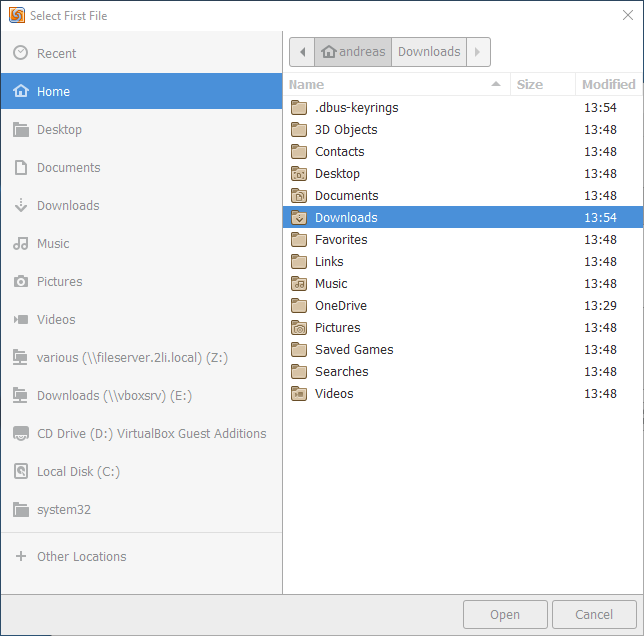
\includegraphics[width=.9\linewidth]{pictures/meld.png}
\caption{\label{fig:orgf6cbe37}
Screenshot der Applikation Meld unter Windows 10}
\end{figure}
Die Gtk Dokumentation empfiehlt \footcite{gtk_setup}, dass man unter Windows das
Programm MSYS2 installiert, um Gtk einzurichten. Zum Programmieren an sich
braucht es offenbar nicht zwingend weitere Tools aus einem Editor. Wie auch bei
Qt hat man jedoch die Möglichkeit das \gls{gui} mit einem \gls{gui} Designer
grafisch zu erstellen.

Wie auch Qt kann man Gtk entweder direkt in der Backend Sprache programmieren
oder aus dem \gls{gui} Designer dann als XML exportieren. Der Code in der
Dokumentation ist in C geschrieben, welches auch nicht die zugänglichste
Sprache ist.

Die Verwendung von Gtk innerhalb des Programms scheint ähnlich einfach zu sein
wie bei Qt. Die Installation ist allerdings unter Windows eher das Gegenteil
von einfach.

Da die Kenntnisse gleich null sind, ist der Lernfaktor auf dem Maximum.

\begin{table}[htbp]
\centering
\begin{tabular}{|>{\columncolor[HTML]{EFEFEF}}p{4cm}|c|p{2cm}|p{2cm}|p{2cm}|}
\hline
\textbf{Kriterium}\cellcolor[HTML]{C0C0C0} & \textbf{Gewichtung}\cellcolor[HTML]{C0C0C0} & \textbf{max. Punktzahl}\cellcolor[HTML]{C0C0C0} & \textbf{erreichte Punktzahl}\cellcolor[HTML]{C0C0C0} & \textbf{Kriteriums- ergebnis}\cellcolor[HTML]{C0C0C0}\\
\hline
1. Cross Plattform nutzbar & 10 & 10 & 10 & 100\\
2. Freie Software & 5 & 10 & 10 & 50\\
3. Vorkenntnisse & 5 & 10 & 0 & 0\\
4. Integriert sich gut ins System & 5 & 10 & 6 & 30\\
5. Ohne spezielle Tools nutzbar & 5 & 10 & 8 & 40\\
6. Lesbarkeit des Codes & 5 & 5 & 3 & 15\\
7. Einfachheit des Setups & 5 & 5 & 3 & 15\\
8. Lernfaktor & 5 & 5 & 5 & 25\\
\hline
\textbf{Total} &  &  &  & 275\\
\hline
\end{tabular}
\caption{\label{tab:orgbb0c6fa}
Gtk Bewertungstabelle}

\end{table}

\paragraph{Electron}
\label{sec:orgd0e93db}

Electron ist ein cross-plattform Framework zum Entwickeln von \glspl{gui} welches
dabei jedoch auf Technologien aus der Webentwicklung benutzt. Entwickelt wird
Electron von der Firma Github und ist \gls{libre} unter der MIT Lizenz
\footcite{electronlicense}.

Da Electron auf Technologien aus der Webentwicklung setzt, sind hier im
Vergleich zu den anderen Frameworks bereit gute Kenntnisse vorhanden. Über die
genau Funktion und Implementierung sind noch keine Kenntnisse vorhanden.

Die Verwendung von Webtechnologien macht Electron zwar sehr kompatibel auf den
unterstützten Systemen, oftmals sehen die Applikationen jedoch doch eher wie
eine Webseite als wie eine Desktop Applikation aus. Ein weiterer Nachteil ist
der hohe Ressourcenverbrauch, da jede Applikation nahezu einer eigenen Instanz
des Google Chrome Browsers gleich kommt.

Bei der Installation muss Node.js und der Paket Manager von Node.js, NPM,
vorhanden sein. Zum Programmieren selber braucht es keine speziellen Tools. Ein
Editor und ein Webbrowser sollten ausreichend sein.

Electron Applikationen bestehen hauptsächlich aus HTML, CSS und JavaScript
Code. Wenn man sich die komplette Applikation in Node.js programmieren möchte
kommt dann noch eine zusätzliche Sprache hinzu. HTML ist ähnlich mühsam zu
lesen wie XML. CSS und JavaScript sind relativ angenehm zu lesen, wobei es für
beide keine offiziellen Styleguides gibt. Was bei Webanwendungen jedoch immer
das schwierigste ist, ist der Wechsel zwischen verschiedenen Sprachen und
Konzepten. Dieses Problem hat man bei Electron leider auch.

Das Setup von Electron ist etwa ähnlich kompliziert wie das Setup von Gtk und
ist sehr ähnlich dem Entwickeln einer normalen Webapplikation.

Da an der IBZ Webtechnologien bereits intensiv behandelt worden sind und man in
diesem Rahmen bereits ein paar Webapplikationen erstellt hat, wäre der
Lernfaktor bei Electron wohl nicht so gross wie etwa bei Qt oder Gtk.

\begin{table}[htbp]
\centering
\begin{tabular}{|>{\columncolor[HTML]{EFEFEF}}p{4cm}|c|p{2cm}|p{2cm}|p{2cm}|}
\hline
\textbf{Kriterium}\cellcolor[HTML]{C0C0C0} & \textbf{Gewichtung}\cellcolor[HTML]{C0C0C0} & \textbf{max. Punktzahl}\cellcolor[HTML]{C0C0C0} & \textbf{erreichte Punktzahl}\cellcolor[HTML]{C0C0C0} & \textbf{Kriteriums- ergebnis}\cellcolor[HTML]{C0C0C0}\\
\hline
1. Cross Plattform nutzbar & 10 & 10 & 10 & 100\\
2. Freie Software & 5 & 10 & 10 & 50\\
3. Vorkenntnisse & 5 & 10 & 5 & 25\\
4. Integriert sich gut ins System & 5 & 10 & 4 & 20\\
5. Ohne spezielle Tools nutzbar & 5 & 10 & 7 & 35\\
6. Lesbarkeit des Codes & 5 & 5 & 3 & 15\\
7. Einfachheit des Setups & 5 & 5 & 3 & 15\\
8. Lernfaktor & 5 & 5 & 3 & 15\\
\hline
\textbf{Total} &  &  &  & 275\\
\hline
\end{tabular}
\caption{\label{tab:orga5779bd}
Electron Bewertungstabelle}

\end{table}

\subsubsection{Ergebnis}
\label{sec:org5625467}

Aufgrund der erreichten Punktzahl, Tabelle:(\ref{tab:org631b7f9}), bei den vorhergehenden
Variantenbewertungen, wurde entschieden für das Backend der Applikation auf
Python zu setzen und fürs Frontend Qt zu benutzen.
\begin{table}[H]
\centering
\begin{tabular}{|>{\columncolor[HTML]{EFEFEF}}p{4.5cm}|r|}
\hline
\textbf{Variante}\cellcolor[HTML]{C0C0C0} & \textbf{Erreichte Punktzahl}\cellcolor[HTML]{C0C0C0}\\
\hline
\textbf{Backend} & \\
C\# & 279\\
C++ & 271\\
Python & 322\\
\textbf{Frontend} & \\
Qt & 295\\
Gtk & 275\\
Electron & 275\\
\hline
\end{tabular}
\caption{\label{tab:org631b7f9}
Variantenbewertung Ergebnis}

\end{table}

\subsection{Applikationsname}
\label{sec:orga32fda6}

Da die einzusetzende Technologie nun feststeht lässt sich auch gut ein Name für
die Applikation ableiten. Oftmals werden die grafischen Applikationen gleich
benannt wie die Kommandozeilen Applikation aber mit dem Namen des \gls{gui}
Frameworks als Suffix. Somit wird das zu erstellende \gls{gui} für \gls{borg} im
weiteren Verlauf der Arbeit nun Borg-Qt genannt

\subsection{Testing}
\label{sec:org85f16b0}

Die Anwendung wird während der Realisierung soweit als möglich mit
automatischen Unittests und Funktionstests überprüft. Dies hauptsächlich um die
Erfahrung in diesem Bereich zu erweitern und um ein gutes Fundament für die
Zukunft des Projektes zu bauen.

Aufgrund der Unerfahrenheit im Bereich des automatisierten Testings wurden noch
die Testfälle in der Tabelle:(\ref{tab:orgd13fe87}), erstellt. Diese werden final von
Hand überprüft. Somit kann vermieden werden das nicht funktionierende
automatische Tests den Abschluss des Projektes verhindern. Da die Testfälle
sich hauptsächlich an den Use Cases orientieren gibt, es ein paar Ziele die,
dadurch nicht getestet werden können. Zudem sind zurzeit nur ca. 20. der Ziele
durch die Use Cases abgedeckt. Die weiteren Ziele lassen sich erst sinnvoll
integrieren, wenn die Basis für das Programm geschaffen wurde. Somit werden
diese Ziele erst im Anschluss zur Diplomarbeit umgesetzt.

Die Ziele, die nicht durch die Testfälle getestet werden können sind Ziel Nr. 1
und Nr. 2. Für Ziel Nr. 1 wird in der Sektion \ref{sec:orgc160c63} ein Proof of Concept
erstellt um die cross-plattform Fähigkeit zu beweisen. Ziel Nr. 2 ist mit
folgendem Link erfüllt. \url{https://github.com/borg-qt/borg-qt/blob/master/LICENSE}.
Dabei handelt es sich um die Lizenz des Borg-Qt Repository.

Getestet wird die Applikation jeweils auf dem Computer des Projektleiters. Auf
diesem läuft die aktuelle Langzeitsupport Version (18.04) von Ubuntu
\footcite{ubuntu} Linux mit der GNOME Desktop Umgebung \footcite{gnome}, als
Betriebssystem. Die Tests werden jeweils gegen eine von PyInstaller generierte
Binärdatei ausgeführt. Der genaue Vorgang der Erstellung dieser Datei wird in
der Sektion: \hyperref[sec:orgf056008]{Releases} beschrieben. Somit werden die Tests immer gegen eine
veröffentlichbare Version gemacht.

Als Testdateien wird jeweils das Code Repository von Borg-Qt selber verwendet.
Der Pfad des \gls{borg} Repository für lokale Backups soll \texttt{/tmp/test-borgqt}
sein, in den Testfällen "`Lokales Repository"', genannt und das Passwort \texttt{foo}.
Im Makefile des Repository wird dieses Setup definiert. Somit kann man als
Entwickler nur \texttt{make init} ausführen und hat eine funktionsfähige Testumgebung.

Um Backups über SSH testen zu können wird eine virtuelle Maschine mit Ubuntu
18.04 verwendet. Die Konfiguration der virtuellen Maschine sieht dabei wie
folgt aus:
\begin{itemize}
\item 2 CPU Kerne
\item 1024 MB RAM
\item IP: 10.7.89.117
\item Ein User \texttt{borg} mit Passwort \texttt{borg}
\item \gls{borg} Repository unter \texttt{/home/borg/backup/diplom} mit Passwort \texttt{foo}, in
den Testfällen "`Server Repository"' genannt
\item Der SSH Key des Entwicklers wird in den User \texttt{borg} importiert. Dies
ermöglicht Passwort freie Logins.
\end{itemize}

Die Testfälle werden während der Entwicklung kontinuierlich durchgeführt. Am
Ende der Diplomarbeit wird das finale Ergebnis des jeweiligen Testfalles
erfasst. Allfällige Besonderheiten werden im Kapitel \hyperref[sec:orgc160c63]{Realisierung}
beschrieben.

\subsection{Klassendiagramm}
\label{sec:org12faf59}

Um die Abhängigkeiten zwischen den einzelnen Klassen der Anwendung aufzuzeigen
wurde ein Klassendiagramm, Abbildung:(\ref{fig:org4ac1491}), erstellt. Das
Klassendiagramm basiert auf dem UML Standard. Im Diagramm wurden nicht alle
"`Properties"' und Methoden alles Klassen aufgezeichnet, sondern nur solche die
auf eine andere Klasse verweisen. Dadurch bleibt das Diagramm übersichtlicher.
Die Klassennamen welche, in fetter Schrift gehalten sind, wurden dabei vom
Projektleiter erstellt. Die Klassennamen, welche kursiv sind, sind Klassen, welche
entweder von Python oder Qt bereitgestellt werden.

\subsection{Benutzerfreundlichkeitsstudie}
\label{sec:orgbeaa226}

Um Borg-Qt auf seine Nutzerfreundlichkeit zu testen wird im Rahmen der
Diplomarbeit noch eine kleine Benutzerfreundlichkeitsstudie gemacht. Bei einer
solchen Studie erhalten die Probanden, Tabelle:(\ref{tab:org825e7b6}), ein paar
Aufgaben, Sektion \ref{sec:orga4d7cc3}, welche sie in einer begrenzten
Zeit zu erledigen haben. Die Aufsichtsperson gibt ihnen dabei keinerlei
Hilfestellungen. Die Probanden sollen die Aufgaben alleine mithilfe der Tipps
und Hinweisen in der Anwendung lösen. Im Anschluss bewerten die Probanden dann
die einzelnen Aufgaben nach ihrer Schwierigkeit,
Tabelle:(\ref{tab:org70a499b}). Daraus lässt sich dann eine sogenannte Heatmap
erstellen. Aus der Heatmap kann man anschaulich herauslesen, welche Bereiche für
die User noch zu kompliziert sind und Nacharbeit benötigen.

Die Probanden wurden aus dem Umfeld des Projektleiters ausgewählt. Es wurde
dabei versucht ein einigermassen breites Spektrum an Computerkenntnissen
abzudecken. Da die Anwendung allen Erfahrungsstufen behilflich sein soll. Die
Angaben in der Tabelle:(\ref{tab:org825e7b6}) sind jedoch die Selbsteinschätzung der
Probanden und nicht die des Projektleiters.

\begin{table}[H]
\centering
\begin{tabular}{|>{\columncolor[HTML]{EFEFEF}}r|c|c|c|c|}
\hline
\textbf{Nr.}\cellcolor[HTML]{C0C0C0} & \textbf{Geschlecht}\cellcolor[HTML]{C0C0C0} & \textbf{Alter}\cellcolor[HTML]{C0C0C0} & \textbf{Englischkenntnisse}\cellcolor[HTML]{C0C0C0} & \textbf{Computerkenntnisse}\cellcolor[HTML]{C0C0C0}\\
\hline
1 & Männlich & 30 & Sehr gut & Sehr gut\\
\hline
2 & Männlich & 26 & Gut & Sehr gut\\
\hline
3 & Männlich & 26 & Gut & Mittel\\
\hline
4 & Männlich & 34 & Mässig & Mittel\\
\hline
5 & Weiblich & 26 & Gut & Mittel\\
\hline
\end{tabular}
\caption{\label{tab:org825e7b6}
Benutzerfreundlichkeitsstudie Probanden}

\end{table}

\begin{table}[H]
\centering
\begin{tabular}{|l|l|}
\hline
\textbf{Grün}\cellcolor[HTML]{4CAF50} & Die Aufgabe war sehr einfach.\\
\hline
\textbf{Gelb}\cellcolor[HTML]{FFEB3B} & Die Aufgabe war etwas herausfordernd.\\
\hline
\textbf{Orange}\cellcolor[HTML]{FF9800} & Die Aufgabe war schwierig.\\
\hline
\textbf{Rot}\cellcolor[HTML]{f44336} & Die Aufgabe war sehr schwierig.\\
\hline
\textbf{Schwarz}\cellcolor[HTML]{424242} & Die Aufgabe war unlösbar.\\
\hline
\end{tabular}
\caption{\label{tab:org70a499b}
Benutzerfreundlichkeitsstudie Bewertungsraster}

\end{table}

\subsubsection{Aufgaben}
\label{sec:orga4d7cc3}

\begin{enumerate}
\item Du möchtest deine Dateien sichern. Erstelle dazu eine Datensicherung des Ordners \texttt{/home/testuser/Downloads}.
\item Du hast aus Versehen die Datei \texttt{/home/testuser/Downloads/Example.pdf}
gelöscht. Stelle die Datei wieder her. Am Ende soll sie unter
\texttt{/home/testuser/Documents/Example.pdf} zu finden sein.
\item Stelle ein beliebiges Archiv wieder her. Der Zielpfad ist \texttt{/home/testuser/Documents/}.
\item Lösche ein Archiv deiner Wahl.
\item Du möchtest das der Ordner \texttt{/home/testuser/Pictures/} nicht mehr gesichert
wird. Konfiguriere die Applikation entsprechend.
\end{enumerate}

\newpage
\subsubsection{Resultate}
\label{sec:orgc096477}

\begin{longtable}{|>{\columncolor[HTML]{EFEFEF}}l|l|l|l|l|l|}
\hline
\textbf{Test}\cellcolor[HTML]{C0C0C0} & \textbf{Proband 1}\cellcolor[HTML]{C0C0C0} & \textbf{Proband 2}\cellcolor[HTML]{C0C0C0} & \textbf{Proband 3}\cellcolor[HTML]{C0C0C0} & \textbf{Proband 4}\cellcolor[HTML]{C0C0C0} & \textbf{Probandin 5}\cellcolor[HTML]{C0C0C0}\\
\hline
\endfirsthead
\multicolumn{6}{l}{Fortsetzung von vorheriger Seite} \\
\hline

\textbf{Test}\cellcolor[HTML]{C0C0C0} & \textbf{Proband 1}\cellcolor[HTML]{C0C0C0} & \textbf{Proband 2}\cellcolor[HTML]{C0C0C0} & \textbf{Proband 3}\cellcolor[HTML]{C0C0C0} & \textbf{Proband 4}\cellcolor[HTML]{C0C0C0} & \textbf{Probandin 5}\cellcolor[HTML]{C0C0C0} \\

\hline
\endhead
\hline\multicolumn{6}{r}{Fortsetzung nächste Seite} \\
\endfoot
\endlastfoot
\hline
1. & \cellcolor[HTML]{4CAF50} & \cellcolor[HTML]{4CAF50} & \cellcolor[HTML]{FFEB3B} & \cellcolor[HTML]{4CAF50} & \cellcolor[HTML]{4CAF50}\\
\hline
2. & \cellcolor[HTML]{FFEB3B} & \cellcolor[HTML]{FFEB3B} & \cellcolor[HTML]{FF9800} & \cellcolor[HTML]{FF9800} & \cellcolor[HTML]{FF9800}\\
\hline
3. & \cellcolor[HTML]{4CAF50} & \cellcolor[HTML]{FFEB3B} & \cellcolor[HTML]{4CAF50} & \cellcolor[HTML]{4CAF50} & \cellcolor[HTML]{4CAF50}\\
\hline
4. & \cellcolor[HTML]{4CAF50} & \cellcolor[HTML]{4CAF50} & \cellcolor[HTML]{4CAF50} & \cellcolor[HTML]{4CAF50} & \cellcolor[HTML]{4CAF50}\\
\hline
5. & \cellcolor[HTML]{4CAF50} & \cellcolor[HTML]{FFEB3B} & \cellcolor[HTML]{FF9800} & \cellcolor[HTML]{FFEB3B} & \cellcolor[HTML]{FFEB3B}\\
\hline
\caption{\label{tab:org223e647}
Benutzerfreundlichkeitsstudie Resultate}
\\
\end{longtable}

\paragraph{Proband 1}
\label{sec:org7a9d191}

Der Proband fand die Aufgaben grundsätzlich einfach zu lösen. Das die "`Mount"'
Funktion zum Wiederherstellen einzelner Dateien gedacht war, hat er nicht
erkannt.

\paragraph{Proband 2}
\label{sec:org2f57971}

Der Proband kam mit den Aufgaben insgesamt gut klar. Bei der ersten Aufgabe
hätte er sich eine Meldung gewünscht, wenn das Backup erfolgreich durchgelaufen
ist. Wie Proband 1 hat auch er die "`Mount"' Funktion nicht genutzt zum
Wiederherstellen einer einzelnen Datei. Text Hinweise wurden nur bedingt
wahrgenommen.

\paragraph{Proband 3}
\label{sec:org82f7ae7}

Proband 3 kam mit der Anwendung an sich gut klar. Die Aufgabe zwei fand er über
alles gesehen auch am schwierigsten, da er mit der Materie nahezu nicht vertraut
ist. Als zusätzlichen Input gab er an, das ein Kontextmenü welches sich mit
Rechtsklick auf ein Element öffnet, etwas sei was er gerne hätte, da er andere
Anwendungen oft so steuert. Aufgabe 5 war auch etwas herausfordernder als 1,3
und 4 insbesondere war unklar wie der Ordner zu der Liste hinzugefügt werden
sollte.

Während des Tests ist in der Anwendung noch ein Bug aufgetaucht, welcher
Probleme beim Erstellen von Archiven machte. Die detaillierte Lösung dafür ist im
Kapitel \ref{sec:orgc160c63} beschrieben.

\paragraph{Proband 4}
\label{sec:orgc2f0473}

Bei Proband 4 war die grösste Hürde dass, das Interface nur in Englisch
verfügbar war. Bei Aufgabe zwei hat er sich nach eigenen Angaben etwas verloren
gefühlt und hätte sich auch ein Kontextmenü auf dem Rechtsklick gewünscht.
Mit etwas Hilfe bei der Übersetzung waren die restlichen Aufgaben jedoch gut zu
meistern.

\paragraph{Probandin 5}
\label{sec:org2277dbc}

Probandin 5 mit der Anwendung insgesamt sehr gut klar und hat auch als Einzige
die Tooltips auf den Buttons entdeckt und dann genutzt. Aufgabe 2 war jedoch
auch schwierig zu lösen, danach ging es jedoch ohne Probleme. Als Feedback wurde
genannt, dass 21:00 Uhr etwas spät für solche Tests sei.

\subsubsection{Auswertung}
\label{sec:orgeea112d}

Nach den 5 Tests liess sich feststellen, dass die Anwendung für die Anwender
insgesamt einfach zu bedienen ist, sobald sie einmal wissen, welche Buttons
welche Aktion auslösen und wie sich die Anwendung verhält. Um Hilfestellung zu
leisten, wird im Rahmen der Diplomarbeit noch ein Hilfefenster eingebaut,
welches den Benutzern beim ersten Starten der Anwendung angezeigt wird und kurz
die jeweiligen Elemente des Interfaces anzeigt. Somit sollte auch das Problem
bei der Aufgabe zwei etwas abgeschwächt werden. Eines der Hauptprobleme war
dort das die Probanden nicht herausgefunden haben der schnellste Weg eine
einzelne Datei wieder herzustellen über die "`Mount"' Funktion ginge. Die
Einarbeitung in die Thematik von Backups würde sich jedoch wohl nur sehr schwer
über das \gls{gui} realisieren lassen. Hier müsste auf jeden Fall eine
Dokumentation oder im Idealfall eine Schulung Abhilfe schaffen.

Das Kontextmenü auf dem Rechtsklick, welches von zwei Usern gewünscht worden
ist, ist eine sehr gute Idee und sollte sich auch realisieren lassen. Dieses
Feature wird nicht im Rahmen der Diplomarbeit umgesetzt und für die zukünftige
Entwicklung aufgenommen.

Ein Dialog, welcher ein erfolgreiches Erstellen eines Archivs bestätigt, wird
nicht eingebaut. Bei erfolgreicher Durchführung verschwindet der
Fortschrittsdialog und in der Archivlist erscheint ein weiterer Eintrag. Das
sind zwar nicht die offensichtlichsten Hinweise im Falle eines Fehlers
erscheint jedoch sofort ein Dialog, der darauf hinweist. Somit sollten die
beiden Vorgänge genügend unterschieden sein und es hat auch kein anderer Proband
das Bedürfnis nach einer Bestätigung.

Für die Zukunft wird eine Deutsche Übersetzung geplant. Dies würde die
Anwendung dann vor allem Leuten mit weniger guten Englisch Kenntnissen
zugänglich machen.

Im Rahmen der Diplomarbeit werden noch einige Texte angepasst. An gewissen
Stellen redet die Anwendung von "`Backups"' und an anderen von "`Archivs"'. Da
\gls{borg} sie selber "`Archives"' nennt, sollte Borg-Qt noch so angepasst werden
das überall von "`Archives"' die Rede ist. Zudem wird bei den "`Include"' und
"`Exclude"' Optionen, über der Liste noch ein Label hinzugefügt, um die Elemente
zu beschreiben. Des Weiteren werden die Buttons "`Add file"' und "`Add folder"' zu
"`Exclude file"' und "`Exclude folder"' sowie "`Include file"' und "`Include folder"'
umbenannt. Somit zeigen die Buttons dann auch direkt, dass sie Dateien
respektive Ordner ein-/ausschliessen Ein paar der Probanden hatten es zuerst
über den "`Remove"' Button versucht.

\section{Realisierung}
\label{sec:orgc160c63}
\subsection{Cross-plattform Kompatibilität}
\label{sec:org5dddaa7}

Um sicherzugehen das die gewählten Technologien auch den Anforderungen
entsprechen wurde ein kleines "`Hello World"' Programm mit Python3 und Qt
geschrieben. Dieses läuft ohne jegliche Probleme und Anpassung auf Windows,
Linux und OS X. Wie in den Screenshots in Abbildung:(\ref{fig:orgdb9cd11}) zu sehen
ist.

\begin{figure}[htbp]
\centering
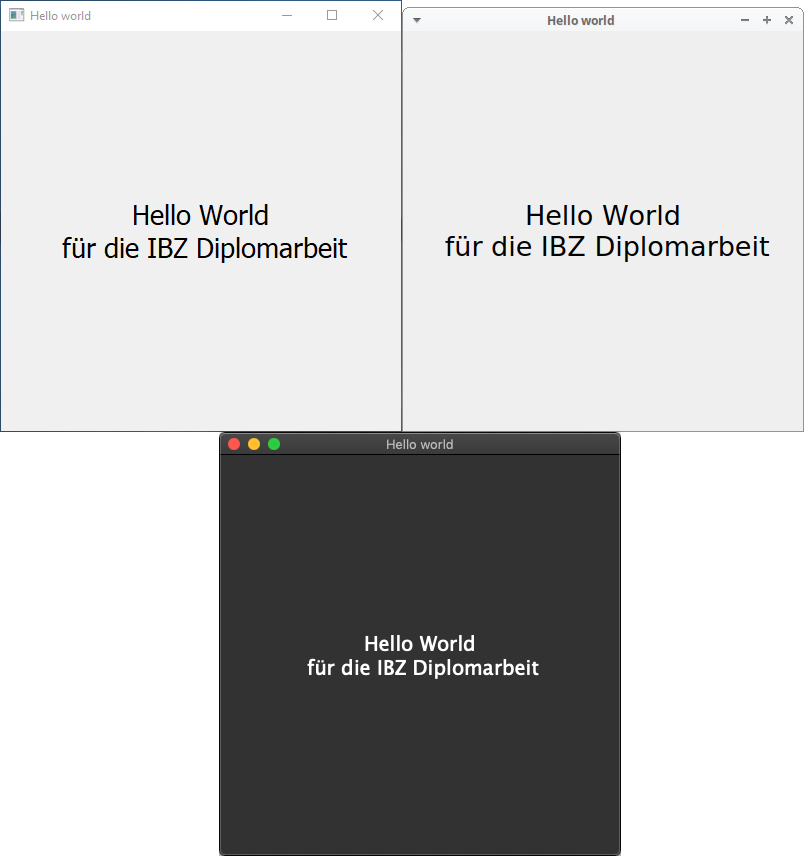
\includegraphics[width=.9\linewidth]{pictures/hello_world.png}
\caption{\label{fig:orgdb9cd11}
Python und Qt Applikation unter Windows (links), Linux (rechts) und OS X (unten)}
\end{figure}

\subsection{Benutzerinterface}
\label{sec:org01da24f}
\subsubsection{Inspiration}
\label{sec:orgbbdb338}

Bevor \gls{borg} vom Projektleiter als Backup Software eingesetzt wurde, nutzte
er die Software "`Back in Time"'\footcite{backintime}. Die Software setzt auf Rsync
zum Kopieren der Dateien. Dies erlaubt auch schnelle Backups über SSH zu
machen. "`Back in Time"' hat allerdings das Problem, dass es keine \gls{dedup}
beherrscht.

Das Userinterface, zu sehen in Abbildung:(\ref{fig:org12a159d}), ist jedoch sehr
gelungen und soll Borg-Qt als Vorlage dienen. Insbesondere die einfache und
direkte Art ein Backup eines spezifischen Pfades zu machen ist sehr gelungen.
Da sie es dem User so einfach wie möglich macht ein Backup zu erstellen.

\begin{figure}[htbp]
\centering
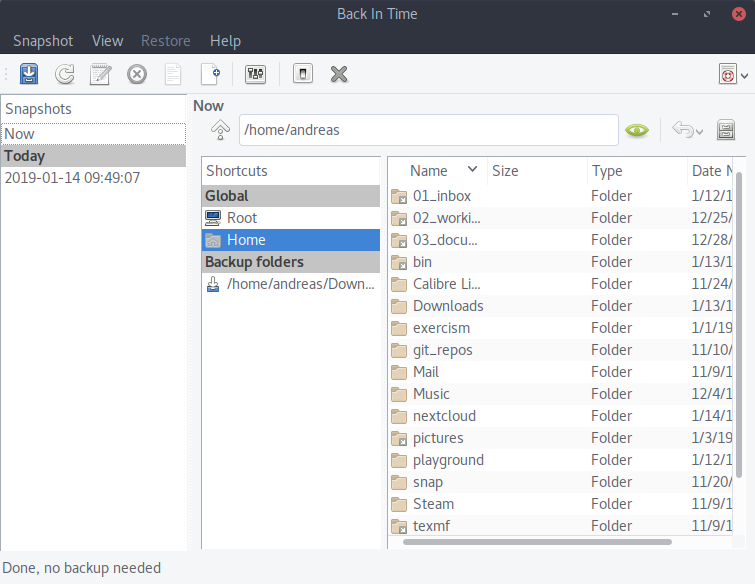
\includegraphics[width=.9\linewidth]{pictures/bit_main.png}
\caption{\label{fig:org12a159d}
Screenshot des Hauptfensters der Software "`Back in Time"'}
\end{figure}

\subsubsection{Erste Umsetzung}
\label{sec:org9949a8a}

Qt bietet einem mehrere Möglichkeiten zum Erstellen der grafischen Oberfläche.
Zum einen kann die ganze Oberfläche programmatisch erstellt werden. Dies gibt
dem Entwickler ein grosses Mass an Kontrolle, ist allerdings nicht sehr
intuitiv.

Die angenehmere Variante ist es den Qt Designer, Abbildung:(\ref{fig:org5dd2144}),
zu nutzen. Mit diesem lassen sich die Oberflächen in einer grafischen
Oberfläche designen und mit einem Befehl auch gleich starten damit man direkt
sieht wie sich die Oberflächen auf dem System verhalten.

\begin{figure}[htbp]
\centering
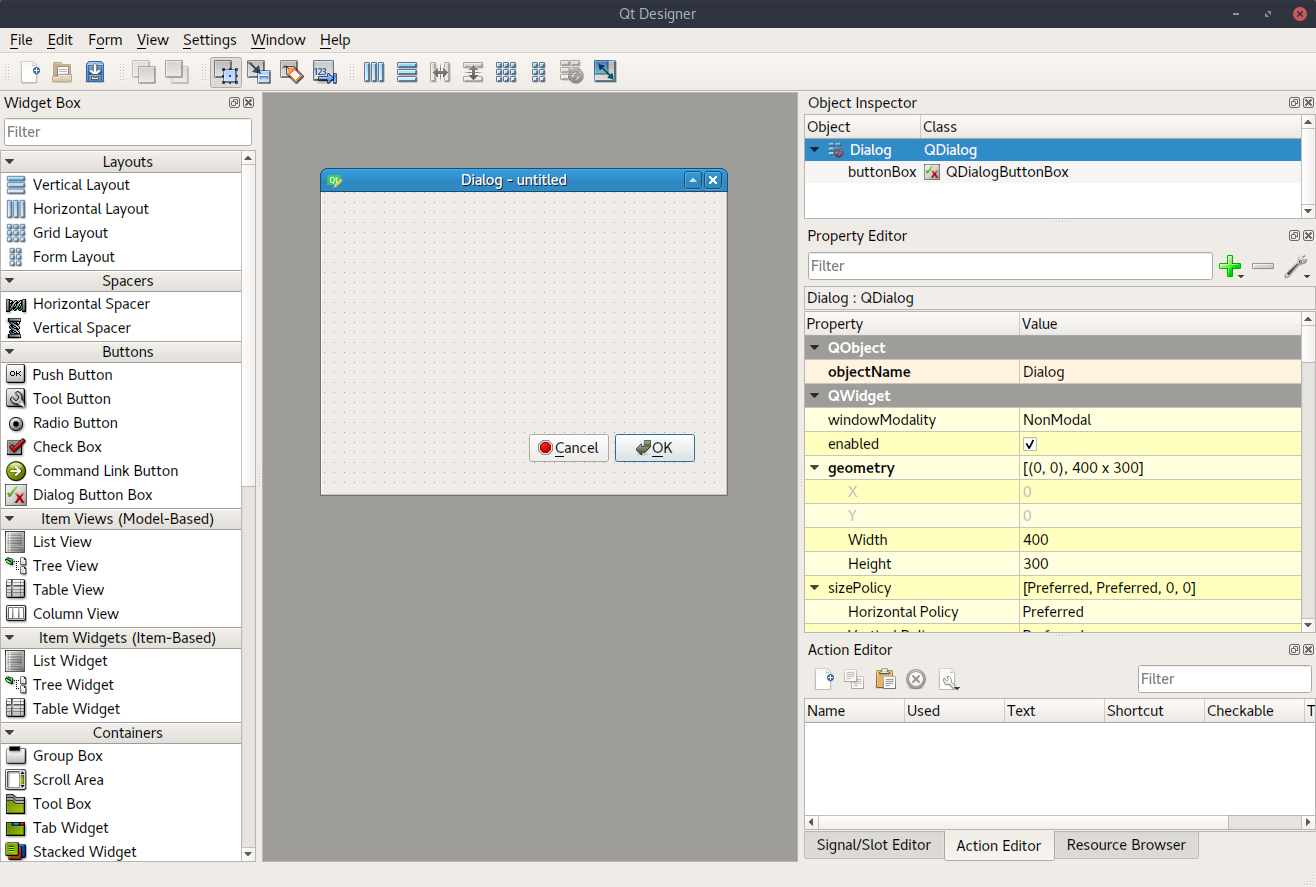
\includegraphics[width=.9\linewidth]{pictures/qt_designer.png}
\caption{\label{fig:org5dd2144}
Ein Screenshot der Applikation Qt Designer}
\end{figure}
Auf Basis der Ziele und der Use Cases wurde eine erste Version des \glspl{gui}
erstellt. Im Hauptfenster, Abbildung:(\ref{fig:org575e47c}), befinden sich wie
auch bei "`Back in Time"' in der einen Hälfte eine Liste der vorhandenen Archive
und in der anderen Hälfte ein Dateimanager. Dieser dient zur Auswahl des zu
sichernden Pfades. Im oberen Bereich findet sich die Toolbar mit den Aktionen,
die der User ausführen kann. Gemäss den Use Cases sind dies "`Backup"',
"`Restore"', "`Mount"', "`Delete"' und "`Settings"'.

Bei den Icons wurde zuerst versucht diese nach der "`Icon Naming
Specification"'\footcite{iconnamespec} auszuwählen. Diese Spezifikationen würden
es erlauben einfach den definierten Namen des Icons anzugeben. Qt würde dann
jeweils das passende Icon basierend auf dem System anzeigen. Somit wären die
Icons passend zum jeweiligen Betriebssystem. Allerdings gab es für die Aktionen
keine passenden Icons in der Spezifikation. Deshalb wurden schlussendlich das
"`Feather"' Icon Theme Set \footcite{feathericons} ausgewählt. Dabei handelt es
sich um ein freies Icon Theme unter der MIT Lizenz, welches die Icons als SVG
Dateien bereitstellt. Dadurch können die Icons frei skalieren und
funktionieren auch auf Geräten mit einer hohen Auflösung.

\begin{figure}[H]
\centering
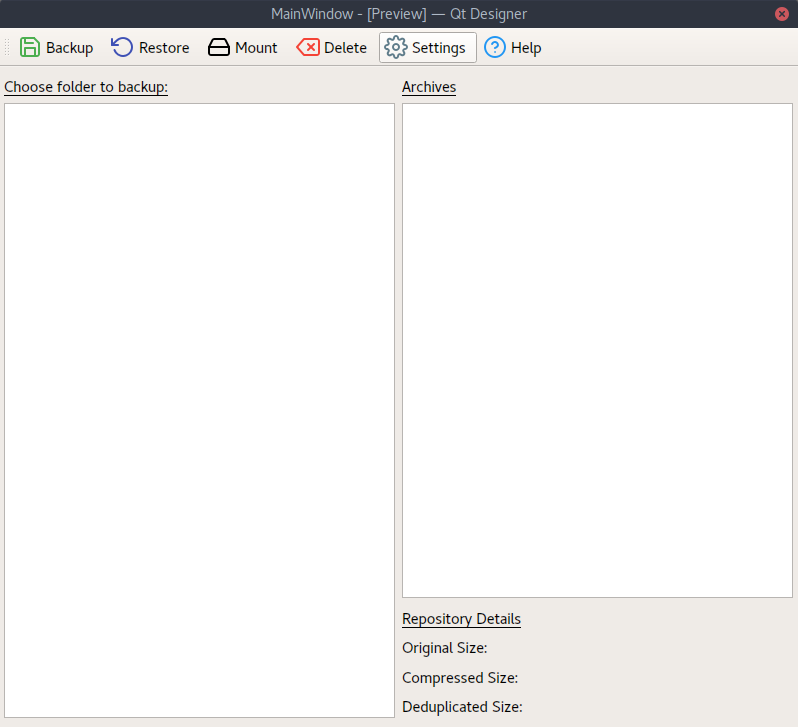
\includegraphics[width=.9\linewidth]{pictures/borgqt_main_v1.png}
\caption{\label{fig:org575e47c}
Screenshot des Borg-Qt Hauptfensters Version 1}
\end{figure}

Im Einstellungsfenster gibt es drei Tabs zur Auswahl. Einmal den "`General"' Tab,
Abbildung:(\ref{fig:orgd6559a6}), dieser zeigt allgemeine Optionen
an. Im zweiten Tab "`Include"', Abbildung:(\ref{fig:orgdbd9f1e}), kann
der User die Ordner und Dateien auswählen, die er sichern will. Der dritte Tab
"`Exclude"', Abbildung:(\ref{fig:org26f570c}), gibt dem User die
Möglichkeit einzelne Ordner oder Dateien von den Backups auszuschliessen.

\begin{figure}[H]
\centering
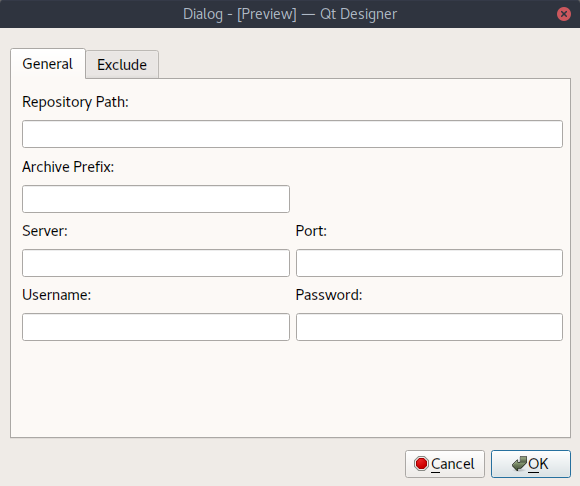
\includegraphics[width=.7\textwidth]{pictures/borgqt_settings_general_v1.png}
\caption{\label{fig:orgd6559a6}
Screenshot der Borg-Qt "`General"' Einstellungen Version 1}
\end{figure}

\begin{figure}[H]
\centering
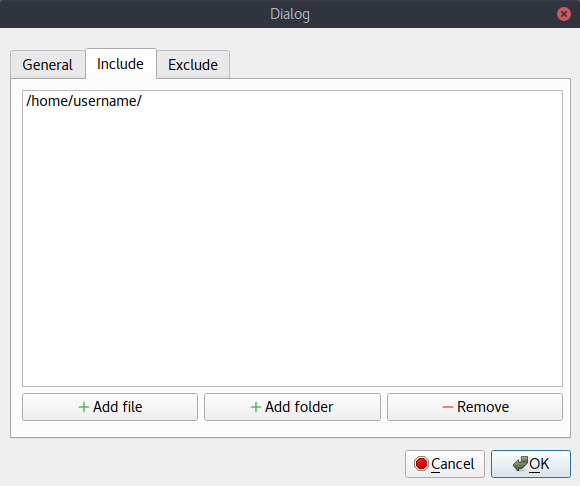
\includegraphics[width=.7\textwidth]{pictures/borgqt_settings_include_v1.png}
\caption{\label{fig:orgdbd9f1e}
Screenshot der Borg-Qt "`Include"' Einstellungen Version 1}
\end{figure}

\begin{figure}[H]
\centering
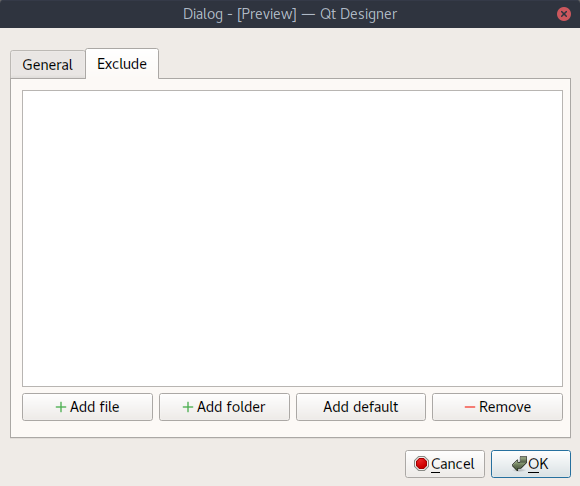
\includegraphics[width=.7\textwidth]{pictures/borgqt_settings_exclude_v1.png}
\caption{\label{fig:org26f570c}
Screenshot der Borg-Qt "`Exclude"' Einstellungen Version 1}
\end{figure}

Das "`Progress"' Dialogfenster, Abbildung:(\ref{fig:org7281322}), zeigt dem
User einen Fortschrittsbalken und einen "`Cancel"' Button zum Abbrechen der
Aktion an. Das Fenster ist generisch gehalten, damit es von verschiedenen Tasks
gleichermassen genutzt werden kann.

\begin{figure}[H]
\centering
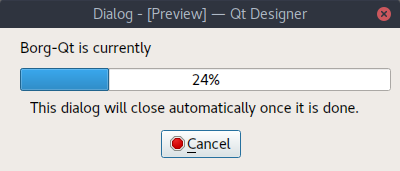
\includegraphics[width=.6\textwidth]{pictures/borgqt_progress_v1.png}
\caption{\label{fig:org7281322}
Screenshot des Borg-Qt "`Progress"' Dialogfensters Version 1}
\end{figure}

\subsection{Einstellungen}
\label{sec:orgc185ba1}

Die Einstellungen werden von der Applikation benötigt, um die vom User
definierten Vorgaben auszuführen, das Backup Repository zu finden, etc.
Diese Einstellungen sollen in einer Klar-Text Datei gespeichert werden. Dies
hat zum einen den Vorteil, dass man die Einstellungen sehr einfach sichern kann.
Zum Anderen kann man die Einstellungen der Applikation auch anpassen, ohne das
man die Applikation selber starten muss.

\subsubsection{Backend}
\label{sec:orgf80b7cd}

Zum Erstellen und Auslesen der Konfigurationsdatei wurde das Python Standard
Modul \texttt{configparser} \footcite{configparser} verwendet. Dieses macht es einem
sehr einfach eine Datei im "`INI"' Stil zu erstellen und parsen.

"`INI"' Stil bedeutet dabei das die Einstellungen in "`Key/Value"' Paaren
gespeichert werden. Somit kann man einfach auf den benötigten Wert zugreifen, in
dem man seinen Schlüssel angibt. Ein Beispiel ist im Code Snippet:
(\ref{orge48e086}) zu sehen.

\lstset{language=bash,label=orge48e086,caption={Ein Beispiel einer INI Datei.},captionpos=b,numbers=none}
\begin{sexylisting}{Ein Beispiel einer INI Datei.}
# docs/borg_qt.conf.example
[borgqt]
includes = [
	    "/home/username/",
        "/home/otheruser/Downloads"
	]
repository_path = /tmp/test-borgqt
password = foo
prefix = muster
\end{sexylisting}

Das Auslesen und schreiben der Konfigurationsdatei liess sicher relativ einfach
realisieren. Die grösste Herausforderung dabei war, das \texttt{Configparser} keinen
Support für eine Liste von Werten hat. Die wurde insbesondere für \texttt{include} und
\texttt{exclude} Pfade benötigt. Also für die Pfade, welche gesichert werden oder von
einem  Backup ausgeschlossen werden sollen.

Abhilfe schaffte hier ein Stackexchange Post \footcite{configlist}. Dieser schlug
vor, das man die Liste im \gls{json} Format speichern soll. Da \texttt{Configparser} alle
Werte im Format "`String"' zurückgibt können dann die \gls{json} Listen sehr
einfach von einem \gls{json} Parser umgewandelt werden. Im Projekt wurde dies
dann unter anderem als Methode der \texttt{Config} Klasse, Code
Snippet:(\ref{orgc9576fb}), implementiert. Somit muss man jeweils nur die
\texttt{\_return\_list\_option()} Methode mit der benötigten Option als Argument aufrufen
und bekommt als Resultat eine funktionierende Python Liste zurück.

Beim Schreiben der Konfigurationsdatei macht man dann einfach das Umgekehrte.
Man konvertiert eine Python Liste in einen \gls{json} String.

\lstset{language=Python,label=orgc9576fb,caption={Methode zum Parsen von \gls{json} Listen in Konfigurationsdateien.},captionpos=b,numbers=none}
\begin{sexylisting}{Methode zum Parsen von gls{json}
# borg_qt/config.py

def _return_list_option(self, option):
    """Reads the provided option from the configparser object and returns
    it as a list."""
    if option in self.config['borgqt']:
        return json.loads(self.config['borgqt'][option])
    else:
        return []
\end{sexylisting}

Die Datei wird jeweils beim Start der Applikation gelesen und angewendet. Somit
weiss die Applikation bereits nach dem Start wo das Repository liegen sollte
und wie die Login Daten dafür sind. Dies geschieht mittels der Methode
\texttt{\_get\_path}, Codesnippet:(\ref{org2ce6f80}). Es gibt dabei zwei mögliche Pfade,
wo die Konfigurationsdatei liegen könnte. Befindet sich die Datei nicht am
vorgegeben Pfad \texttt{\textasciitilde{}/.config/borg\_qt/borg\_qt.conf} oder direkt "`neben"' dem
Binary, gibt die Applikation eine entsprechende Meldung,
Abbildung:(\ref{fig:orgcd4efa1}), aus. Der Hauptpfad unter
\texttt{\textasciitilde{}/.config/borg\_qt/borg\_qt.conf} wird dabei gemäss dem Ziel Nr. 21 über die
Umgebungsvariable \texttt{HOME} zusammengesetzt

\lstset{language=Python,label=org2ce6f80,caption={Methode zum Suchen der Konfigurationsdatei},captionpos=b,numbers=none}
\begin{sexylisting}{Methode zum Suchen der Konfigurationsdatei}
# borg_qt/config.py

def _get_path(self):
    """searches for the configuration file and returns its full path."""
    home = os.environ['HOME']
    dir_path = os.path.dirname(os.path.realpath(__file__))

    if os.path.exists(os.path.join(home, '.config/borg_qt/borg_qt.conf')):
        return os.path.join(home, '.config/borg_qt/borg_qt.conf')
    elif os.path.exists(os.path.join(dir_path, 'borg_qt.conf')):
        return os.path.join(dir_path, 'borg_qt.conf')
    else:
        raise BorgException("Configuration file not found!")
\end{sexylisting}

\begin{figure}[H]
\centering
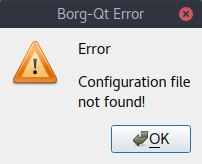
\includegraphics[width=.3\textwidth]{pictures/borgqt_missing_config.png}
\caption{\label{fig:orgcd4efa1}
Screenshot der Borg-Qt Fehlermeldung bei fehlender Konfigurationsdatei.}
\end{figure}

\subsubsection{Frontend}
\label{sec:orga2421c7}

Um es für die User einfacher zu machen wurde beschlossen die Applikation,
um eine grafische Konfigurationsmöglichkeit zu erweitern. Diese stellt dabei
hauptsächlich die Werte aus der Konfigurationsdatei grafisch dar und übergibt
allenfalls geänderte Werte ans Backend welches die Konfiguration, dann wieder in
der Datei speichert.

Das Meiste davon ist nicht besonders aufregender Code da hauptsächlich nur die
Werte aus der Konfigurationsdatei in die entsprechenden Textfelder und Listen
im grafischen Interface geschrieben werden auch beim Speichern der geänderten
Einzel-Werte funktioniert es in etwa gleich. Beim Speichern der geänderten
Listen jedoch trat eine weitere Herausforderung auf.

Qt kennt keinen Mechanismus zum Auslesen aller Elemente aus einem sogenannten
\texttt{QListWidget}, einem \gls{gui} Element, welches Listen darstellt. Somit ist es
nötig das man die Elemente zuerst in einer Zwischenliste speichert bevor man
sie zurück in das \texttt{Configparser} Objekt schreiben kann. Im Code sieht dies dann
wie in Codesnippet:(\ref{org98b3049}) aus. Dabei wird jedes Element
einzeln aus dem \texttt{QListWidget} geholt und in die Zwischenliste geschoben. Im
zweiten Teil wird die Liste dann wieder zu einem \gls{json} String konvertiert
und im \texttt{Configparser} Objekt gespeichert. Die Option \texttt{indent=4} dient dabei der
Lesbarkeit damit nicht der ganze \gls{json} String auf ein Zeile in der
Konfigurationsdatei gespeichert wird, sondern jedes Listenelement seine eigene
Zeile erhält.

\lstset{language=Python,label=org98b3049,caption={Workaround zum Auslesen aller Elemente in QListWidgets.},captionpos=b,numbers=none}
\begin{sexylisting}{Workaround zum Auslesen aller Elemente in QListWidgets.}
# borg_qt/config.py

# Workaraound to get all items of a QListWidget as a list
includes = []
for index in range(self.list_include.count()):
    includes.append(self.list_include.item(index).text())

# Configparser doesn't know about list therefore we store them as json
# strings
self.config['borgqt']['includes'] = json.dumps(includes,
                                               indent=4,
                                               sort_keys=True)
\end{sexylisting}

\subsection{Borg Interface}
\label{sec:orgd904704}

Zuerst erschien es sinnvoll die Kommunikation zwischen \gls{borg} und Borg-Qt
über einfache Funktionen laufen zu lassen. Dieser Ansatz hatte allerdings zwei
Probleme. Zum einen wurde es relativ umständlich Informationen zu verarbeiten
und weiterzugeben zum anderen führte es zu dem unschönen Nebeneffekt dass, das
\gls{gui} eingefroren ist. Eine Recherche ergab, dass Threads hier Abhilfe
schaffen könnten.

Python würde hierzu ein Modul, \texttt{threading.Thread} \footcite{threading},
mitliefern. Allerdings war es nicht möglich den Fortschrittsdialog und den
Thread so zu verknüpfen das sich der Dialog schliesst, wenn das Backup
durchgelaufen ist und der Thread wieder entfernt wird. Aus diesem Grund wurde
dann ein erfolgreicher Test mit dem PyQt Modul \texttt{QThread} \footcite{qthread}
gemacht. Mit diesem war es ohne weiteres möglich den Dialog zu schliessen,
sobald das Backup fertig durchgelaufen war. Auch das Stoppen des Threads mit
einem Klick auf den "`Cancel"' Button funktioniert einwandfrei.

Damit \gls{borg} aus der Anwendung angesteuert werden kann wird das Python Modul
\texttt{subprocess} \footcite{subprocess} verwendet. Dieses erlaubt einem neue Prozesse
zu erstellen, welche man oftmals benötigt um etwa, wie im Fall von Borg-Qt,
externe Applikationen zu starten, zu steuern und ihre Ausgabewerte auszulesen.
Das effektive Kommando wird dann aus dem Property \texttt{self.command} gelesen.

Damit \gls{borg} die Ausgabe im \gls{json} Format ausgibt, muss man man noch die
Parameter \texttt{-{}-log-json} und \texttt{-{}-json} mitgeben. Der erste Parameter ändert
hauptsächlich das Format von Errormeldungen und der zweite formatiert dann die
finale Ausgabe. Die Ausgaben werden jeweils an Variablen weitergegeben
(\texttt{json\_output} und \texttt{json\_error}) welche im weiteren Code verarbeitet werden.

Insbesondere \texttt{json\_error} ist für den weiteren Programmablauf von grosser
Wichtigkeit. Wenn Borg ein Problem feststellt, wird die Error Meldung von
\gls{borg} an \texttt{json\_error} weitergegeben. Mittels der Methode im
Codesnippet:(\ref{orgbe8048f}), wird die Variabel ausgewertet und im Falle eines
Fehlers wirft der Code eine Exception, welche im Hauptprogramm abgefangen wird.
Dabei wird eine Fehlermeldung in einem separaten Fenster ausgegeben. Die
Methode wurde dabei auf der Klasse \texttt{BorgQtThread} umgesetzt und steht somit
allen Funktionen zur Verfügung. Die Fehlermeldung bei einer fehlenden
Konfigurationsdatei, Abbildung:(\ref{fig:orgcd4efa1}), funktioniert nach
dem gleichen Prinzip und konnte somit zum grössten Teil wiederverwendet werden.
Der restliche \gls{json} Output kann dann einfach mit dem \texttt{json} Modul geparst
werden. Somit werden dem User, gemäss Ziel Nr. 14, direkt die Fehlermeldungen
von \gls{borg} angezeigt und es muss nur an gewissen Stellen noch
applikationsspezifisches Exception Handling betrieben werden.

\lstset{language=Python,label=orgbe8048f,caption={Auswertung der json err Variabel.},captionpos=b,numbers=none}
\begin{sexylisting}{Auswertung der json err Variabel.}
# borg_qt/borg_interface.py

def process_json_error(self, json_err):
    if json_err:
        error_list = json_err.split('\n')
        if "borg.locking" in error_list[0]:
            pass
        else:
            err = json.loads(error_list[0])
            raise BorgException(err['message'])
\end{sexylisting}

Die ganze Funktionalität wurde dann in der Klasse \texttt{BorgQtThread}
zusammengefasst. Somit kann für jede Funktion von \gls{borg} eine einzelne Klasse
geschrieben werden, welche dann von \texttt{BorgQtThread} die Funktionen erbt. Die
Funktionsklassen müssen dann jeweils nur die Methode
\texttt{self.create\_command(self)} implementieren welche das Property \texttt{self.command}
erstellt und die einfachen Funktionen von \gls{borg} sollten direkt funktionieren

\subsection{Backup}
\label{sec:org7ad98eb}

Bei den Backups handelt es sich ohne Zweifel um die wichtigste Funktion von
Borg-Qt. Deshalb soll das Erstellen eines Backups so schnell und unkompliziert
wie möglich vonstattengehen.

\subsubsection{Backend}
\label{sec:org1f2a8e9}

Um Backups erstellen zu können wurde die Klasse \texttt{BackupThread} erstellt, welche
von \texttt{BorgQtThread} erbt. Die Klasse \texttt{BackupThread} nimmt beim instantiieren 3
Argumente auf: \texttt{includes}, \texttt{excludes}, \texttt{prefix}. Wobei \texttt{excludes} und \texttt{prefix}
beide optional sind. Im Hauptcode werden diese Argumente aus der
Konfigurationsdatei ausgelesen und übergeben. Die Includes werden im Falle
eines Backups im Hintergrund aus der Konfigurationsdatei gelesen. Wenn es
der User manuell ausführt, wird der im Frontend ausgewählte Pfad mitgegeben.

Die "`Excludes"' haben lange nicht funktioniert. Der Grund dafür waren zusätzliche
Anführungszeichen um die Exclude Pfade. Diese wurden aus Versehen hinzugefügt
da \gls{borg} normalerweise auf der Kommandozeile ausgeführt wird und die
Anführungszeichen dort notwendig sind um allfällige Leer- oder Sonderzeichen
abzufangen. Es wurde davon ausgegangen dass, da \texttt{subprocess} Modul ähnlich
funktioniert wie die Kommandozeile. Da man an das Modul direkt einen String
übergibt, sind die zusätzlichen Anführungszeichen nicht notwendig und führen
sogar dazu das die Pfade gar nicht funktionieren. Somit werden die "`Excludes"'
mittels der Methode \texttt{\_process\_excludes} mit dem entsprechenden Parameter
gepaart und als gesamte Liste an das finale Kommando angehängt. Die "`Includes"'
funktionieren auf die gleiche Weise, benötigen jedoch keine zusätzlichen
Parameter. Zu sehen ist dies im Codesnippet:(\ref{orgacbd2ca}).

\lstset{language=Python,label=orgacbd2ca,caption={Erstellen des "`borg create"' Kommandos fürs erstellen von Backups.},captionpos=b,numbers=none}
\begin{sexylisting}{Erstellen des "`borg create"' Kommandos fürs erstellen von Backups.}
# borg_qt/borg_interface.py
# Funktion zum Verarbeiten der "Excludes"
def _process_excludes(self, excludes):
    processed_items = []
    if excludes:
        for item in excludes:
            processed_items.extend(['-e', item])
        return processed_items
    else:
        return processed_items

# Methode zum Erstellen des gls:borg Kommandos.
def create_command(self):
    self.command = ['borg', 'create', '--log-json', '--json',
                    ('::'
                        + self.prefix
                        + '{now:%Y-%m-%d_%H:%M:%S}')]
    self.command.extend(self.includes)
    if self.excludes:
        self.command.extend(self.excludes)
\end{sexylisting}

\subsubsection{Frontend}
\label{sec:orgbd48c28}

Damit die Backups im Frontend funktionieren musste zum einen der "`Backup"' Knopf
mit der Methode \texttt{create\_backup} verknüpft werden. Des Weiteren wurde ein Dateibaum, in
Abbildung:(\ref{fig:orgebca5ba}) grün umrahmt, eingefügt. Dieser gibt den Pfad
des angewählten Objektes and die \texttt{create\_backup} Methode weiter.

\begin{figure}[htbp]
\centering
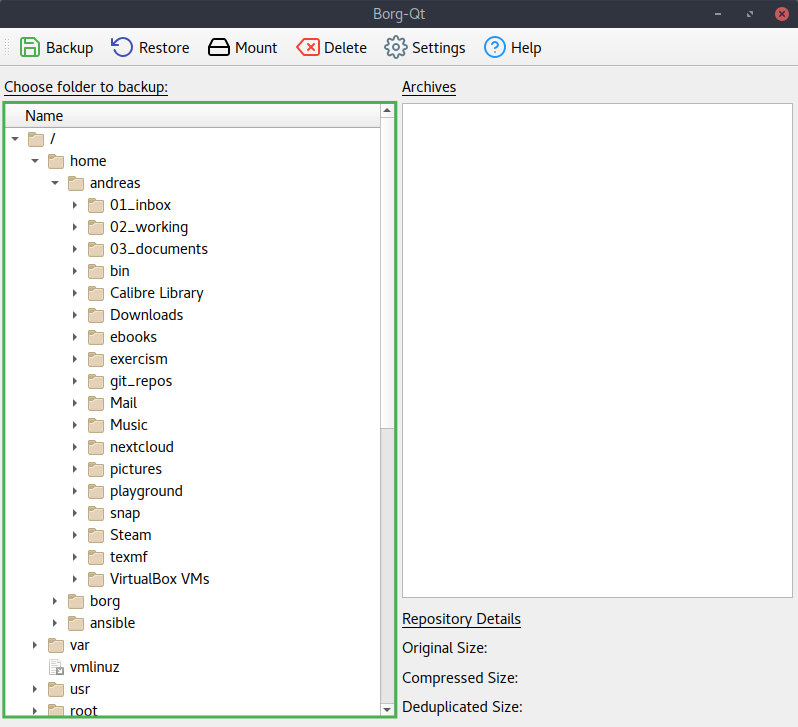
\includegraphics[width=.9\linewidth]{pictures/borgqt_file_tree.png}
\caption{\label{fig:orgebca5ba}
Screenshot des Dateibaumes.}
\end{figure}

Während dem ein Archiv erstellt wird, wird ein kleiner Dialog mit Ladebalken
angezeigt, Abbildung:(\ref{fig:org973d4de}). Dieser dient hauptsächlich dazu
dem User das Gefühl zu geben, das die Applikation noch am Arbeiten ist.

Der Dialog musste gegenüber der ersten Version in Sektion: \hyperref[sec:org9949a8a]{Erste Umsetzung} noch
etwas angepasst werden. \gls{borg} gibt, während dem Erstellen eines Archivs
keine Informationen zurück, welche es einem erlauben würden einen
Fortschrittsbalken zu generieren, welcher den effektiven Fortschritt anzeigt.
\gls{borg} gibt einzig die Anzahl der verarbeiteten Dateien in regelmässigen
Abständen zurück. Da \gls{borg} jedoch zu Beginn nicht meldet wie viele Dateien
gesichert werden lässt sich damit keine Prozentzahl erstellen. Ein paar
Experimente, bei denen die zu sichernden Dateien zuerst von Borg-Qt gezählt
werden sollten, wurden verworfen. Einerseits weil keine Methode gefunden werden
konnte, welche die gleiche Anzahl Dateien zurückgab wie \gls{borg}. Anderseits,
weil es den Backup Vorgang unnötig in die Länge zieht. Dies ist insbesondere
der Fall, wenn sich sehr viele Dateien im Quellverzeichnis befinden. Es kann
sogar soweit kommen dass, das Zählen länger als das eigentliche Sichern dauert.
Aus diesem Grund wurde der Fortschrittsbalken mit Prozentanzeige durch einen
sich wiederholenden Ladebalken ersetzt.

\begin{figure}[H]
\centering
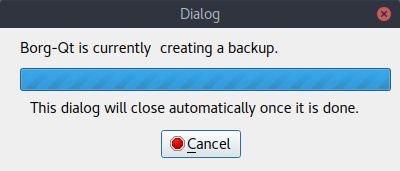
\includegraphics[width=.4\paperwidth]{pictures/borgqt_progress_v2.png}
\caption{\label{fig:org973d4de}
Screenshot des "`Aktion in Ausführung"' Dialogs.}
\end{figure}

Wurde das Archiv erfolgreich erstellt, wird die Liste mit den Archiven sowie
die Repository Statistik aktualisiert. Beide Elemente sind in der,
Abbildung:(\ref{fig:org5e3466a}), grün respektive rot umrahmt. Für die
beiden Funktionen wurde jeweils eine eigene Klasse, \texttt{ListThread} und
\texttt{InfoThread}, erstellt. Beide erben von \texttt{BorgQtThread}. In den Klassen wird wie
bei \texttt{BackupThread} \gls{borg} über einen \texttt{subprocess} aufgerufen, um die Archiv Liste
respektive Statistik zurückzuerhalten Die \gls{json} Strings werden wieder auf
die jeweilige Information geparst und die Archive in eine Python List, die
Repository Statistik in Zahlen umgewandelt.

Da \gls{borg} die Repository Grössen in Bytes zurückgibt, sollten diese zur
Anzeige noch in eine Menschen lesbarses Format umgerechnet werden. In Borg-Qt
geschieht dies mit der Helferfunktion \texttt{convert\_size}. Die Funktion wurde von
Stackoverflow \footcite{sizeformat} übernommen.

Beim Durchführen der Benutzerfreundlichkeitsstudie wurde noch ein Bug entdeckt.
Der Bug, der entdeckt wurde, tritt immer dann auf, wenn ein Archiv gemountet
ist während man ein Backup erstellen möchte. Dies ist jedoch offenbar eine
Funktion die von \gls{borg} nicht unterstützt wird \footcite{borgmount}. \gls{borg}
kann mehrere Archive gleichzeitig mounten. Der User müsste jedoch jedes der
Archive zuerst wieder unmounten bevor er eine neue Datensicherung erstellen
kann. Das Problem wurde dadurch gelöst das dem User ein Dialog angezeigt wird,
über welchen er vor einer Datensicherung zuerst die gemounteten Archive
aushängen kann. Anschliessend startet die Datensicherung wie, wenn kein
Archiv gemountet gewesen wäre.

\begin{figure}[htbp]
\centering
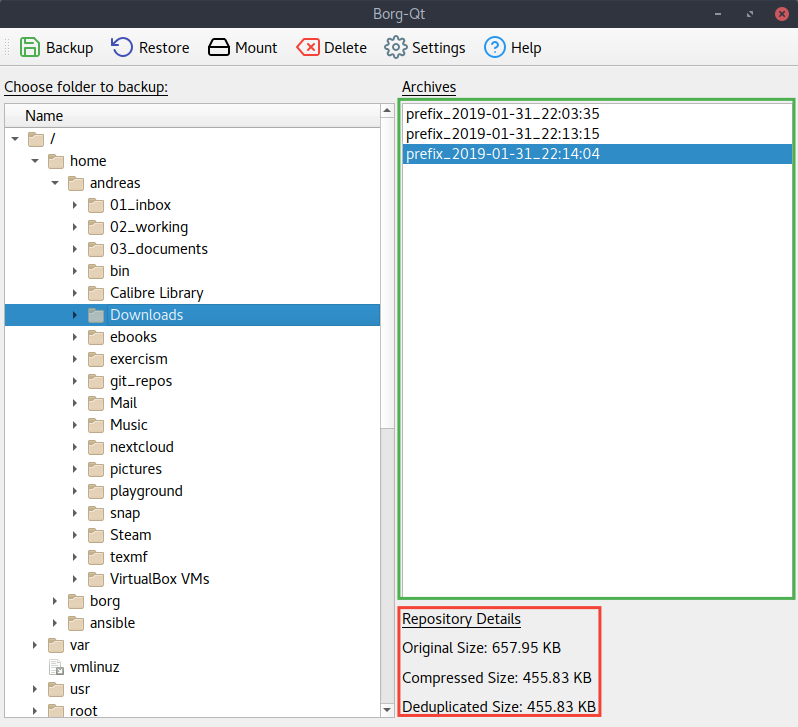
\includegraphics[width=.9\linewidth]{pictures/borgqt_archive_list.png}
\caption{\label{fig:org5e3466a}
Screenshot der aktualisierten Archivliste und Repository Statistik.}
\end{figure}

\subsection{Restore}
\label{sec:orgb888cf7}

Der Code für das Wiederherstellen eines Backups ist sehr ähnlich wie der Code
für das Erstellen. Die Besonderheiten bei dieser Funktion sind vor allem, die
Kontrolle das ein Archiv angewählt wurde bevor man die Wiederherstellung
startet, das Erstellen des Zielpfades sowie das Aufräumen bei einem Fehler.

Wird der "`Restore"' Knopf gedrückt ohne das ein Backup angewählt wurde, erscheint
folgende Fehlermeldung, Abbildung:(\ref{fig:org0cafd47}), um den Benutzer
darauf hinzuweisen, das er dies noch tun sollte.

\begin{figure}[H]
\centering
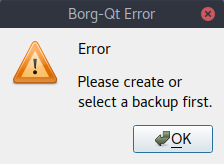
\includegraphics[width=.2\paperwidth]{pictures/borgqt_no_archive_selected.png}
\caption{\label{fig:org0cafd47}
Screenshot der Fehlermeldung eines fehlenden Archivs während einem Restore.}
\end{figure}

Das Wiederherstellen an sich läuft so ab das der Benutzer zuerst ein Archiv
auswählt und dann auf "`Restore"' klickt. Daraufhin öffnet sich ein Dialog, in
welchem der Benutzer den Zielort auswählen kann. Sobald er dies getan hat
erstellt Borg-Qt darin einen Order mit dem Namen des Archivs und beginnt mit
dem eigentlichen Wiederherstellen. Sollte der Zielort für die Applikation nicht
beschreibbar sein erscheint eine entsprechende Fehlermeldung,
Abbildung:(\ref{fig:org3dcb5db}), und der Vorgang wird abgebrochen. Nach einer
erfolgreichen Wiederherstellung öffnet die Applikation den Zielort in einem
Dateimanager, damit der User gleich mit den Dateien weiterarbeiten kann.

\begin{figure}[H]
\centering
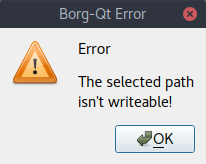
\includegraphics[width=.2\paperwidth]{pictures/borgqt_not_writeable.png}
\caption{\label{fig:org3dcb5db}
Screenshot der Fehlermeldung wenn der Zielort nicht beschreibbar ist.}
\end{figure}

Gibt es, während dem Wiederherstellen einen Fehler gibt die Anwendung den
entsprechenden Fehler aus und löscht zusätzlich noch den zu Beginn erstellten
Archiv Ordner. Dies aus dem Grund da die Wiederherstellung ja nicht komplett
durchgelaufen ist, somit befindet sich das Archiv in einem unfertigen Zustand.
Es ist deshalb sinnvoller die wiederhergestellten Dateien wegzuräumen als unter
Umständen defekte Dateien zurückzulassen

Wird das gleiche Archiv nochmal an den gleichen Zielort wiederhergestellt, ist
das für \gls{borg} kein Problem. Es überschreibt die Dateien einfach noch einmal

\subsection{Mount}
\label{sec:org414f8a8}

Die "`Mount"' Funktion ist sehr ähnlich wie die "`Restore"' Funktion. Sie prüft
auch zuerst ob der Benutzer überhaupt ein Archiv angewählt hat und gibt, falls
dies nicht der Fall ist eine entsprechende Fehlermeldung aus. Im Gegensatz zur
"`Restore"' Funktion zeigt die "`Mount"' Funktion jedoch keinen Dialog zum
Auswählen des Zielpfades. Die Funktion erstellt sich diesen selbst. Der
Zielpfad ist dabei kombiniert aus dem \texttt{/tmp} Verzeichnis und dem Namen des
Archivs

\gls{borg} mountet jedes Archiv nur mit Leserechten. Es ist relativ
unwahrscheinlich, dass der Zielpfad in unbeschreibbarer Form bereits vor dem
Ausführen der \texttt{mount\_backup} Methode bereits vorhanden ist. Sollte dies jedoch
der Fall sein kann davon ausgegangen werden das der Benutzer das Archiv bereits
einmal gemountet hat. Genau dies wird in der Applikation auch so überprüft.
Falls der Zielort schreibbar ist, wird das ausgewählte Archiv auf diesem Pfad
gemountet. Anschliessend wird wie auch bei der Restore Funktion, der Pfad in
einem Dateimanager geöffnet damit der Benutzer direkt mit den Dateien
weiterarbeiten kann. Wurde erkannt dass, das Archiv bereits gemountet wurde,
also der Pfad nicht schreibbar ist, öffnet die Applikation direkt den
Dateimanager ohne zu versuchen das Archiv noch einmal zu mounten.

Zusätzlich wird der Pfad jedes gemounteten Archivs in einer Liste gespeichert.
Beim Beenden der Applikation iteriert die Applikation über jeden Pfad in der
Liste unmountet das Archiv und löscht den Ordner. Somit befindet sich das
System wieder im gleichen Zustand wie vor dem Start der Applikation.

\subsection{Delete}
\label{sec:org33428e5}

Der Benutzer hat in der Applikation auch die Möglichkeit Archive wieder zu
löschen. Hierbei greift wie bei der "`Restore"' und "`Mount"' Funktion auch wieder
die Überprüfung ob der Benutzer ein Archiv ausgewählt hat. Ist dies gegeben,
zeigt die Applikation dem Benutzer einen Dialog, Abbildung:(\ref{fig:orgecbafd9}), zum
Sicherstellen, dass er das Archiv wirklich löschen möchte. Bestätigt er diesen
mit "`Yes"' wird der Vorgang fortgesetzt und das Archiv gelöscht. Anschliessend
werden die Archivliste und die Repository Statistik aktualisiert, um den neuen
Zustand wiederzugeben. Klickt der Benutzer stattdessen auf "`No"' schliesst sich
der Dialog wieder und nichts weiter passiert.

\begin{figure}[H]
\centering

\includegraphics[width=.3\paperwidth]{pictures/borgqt_yes_no.png}
\caption{\label{fig:orgecbafd9}
Screenshot des Yes/No Dialogs in der "`Delete"' Funktion.}
\end{figure}

\subsection{Automatische Backups}
\label{sec:orgff72e08}

Damit der Benutzer die Backups von Hand machen muss, ist es sinnvoll eine
Funktion bereitzustellen, welche die Backups automatisch im Hintergrund
erledigt. Dadurch ist sichergestellt das die Backups im allgemeinen Trubel des
Lebens nicht vergessen gehen.

Damit automatische Backups überhaupt möglich sind muss die Applikation zuerst
Backups im Hintergrund erstellen können, also ohne das die ganze grafische
Oberfläche angezeigt wird. Bei Borg-Qt wird dies über einen Kommandozeilen
Parameter realisiert. Hierfür wurde das Python Standard Paket \texttt{argparser}
verwendet. Konkret bedeutet dies, dass wenn man die Applikation auf
der Kommandozeile wie folgt ausführt: \texttt{borg\_qt -B}. Wird die grafische Oberfläche
nicht angezeigt und es wird direkt die Methode \texttt{background\_backup} der Klasse
\texttt{MainWindow} ausgeführt. Dabei werden alle Ordner, welche in den Einstellungen
unter "`Include"' sowie "`Exclude"' gespeichert wurden, im Archiv gesichert,
respektive davon ausgeschlossen. Damit sind die Voraussetzungen für
automatische Backups gegeben.

Um die Backups in regelmässigen Intervallen auszuführen, gibt es zwei
Möglichkeiten, wie man dies implementieren könnte. Zum einen könnte man die
Applikation permanent im Hintergrund laufen lassen, etwa als Trayicon wie man
das von anderen Applikationen wie etwas Dropbox kennt zum anderen kann man es
über Werkzeuge des Betriebssystems bewerkstelligen. Die drei
Desktop Betriebsysteme, Windows, OS X und Linux, bringen alle drei Werkzeuge
mit, um periodisch ein Programm auszuführen. Unter Linux wurde dies früher mit
sogenannten Cron Jobs gemacht. Die moderne Lösung sind heutzutage jedoch
Systemd Timer. Für Borg-Qt wurde beschlossen es mit den Werkzeugen des
Betriebssystems zu machen. Also konkret Systemd. Dies aus dem Grund das Systemd
genau für das Managen von Applikationen programmiert wurde. Ein Grossteil der
Funktion ist bereits in Systemd enthalten, somit kann man Zeit sparen. Zudem
soll die Anwendung dem Benutzer auch soweit als möglich aus dem Weg gehen. Eine
Applikation, welche permanent in der Taskleiste lebt scheint hier nicht wirklich
das Kriterium zu erfüllen.

Systemd ist ein init System, welches dazu dient dazu die Benutzerumgebung und
die dazugehörigen Prozesse zu starten und zu verwalten \footcite{systemd}. Die
Prozesse werden über sogenannte "`Services"' gestartet. Die Services werden dabei
einfach in Klartextdateien mit der Dateiendung \texttt{.service} definiert. Der Inhalt
orientiert sich dabei praktischerweise am "`INI"' Stil. In Borg-Qt wurde das INI
Format bereits bei den Konfigurationsdateien verwendet. Somit können dort
gesammelte Erfahrungen wiederverwendet werden. Soll ein Service in einem
gewissen Zeitintervall ausgeführt werden benötigt Systemd eine weitere Datei mit
dem gleichen Namen jedoch mit der Dateiendung \texttt{.timer} . Der Inhalt ist auch
wieder im INI Stil gehalten. Systemd versteht eine Vielzahl an Datumsformaten
\footcite{systemddate}. In Borg-Qt wurden zwei Varianten in den Einstellungen
umgesetzt. Eine, welche "`Predefined Schedule"' genannt wurde und eine mit dem
Namen "`Custom Schedule"', zu sehen in, Abbildung:(\ref{fig:org4597de1}). Die Predefined
Option wird dabei in die von Systemd unterstützten Formate "`hourly"', "`daily"',
"`weekly"' und "`monthly"' übersetzt. Wie der Name schon sagt, wird dann stündlich,
täglich, wöchentlich oder monatlich ein Archiv erstellt. Mit der Custom Option
kann der Benutzer sich den Zeitplan individueller gestalten. Etwa "`jeden
Mittwoch um 12:00 Uhr"' für Systemd übersetzt würde dieser Zeitplan dann so
aussehen: \texttt{Wednesday *-*-* 12:00:00}. Für spätere Versionen von Borg-Qt wäre es
allenfalls auch möglich die Auswahl von mehreren Wochentagen zu ermöglichen
damit der Benutzer etwa folgenden Zeitplan erstellen könnte "`Montag, Mittwoch,
Freitag stündliche Backups."' (\texttt{Monday, Wednesday, Friday *-*-* *:00:00}).

\begin{figure}[H]
\centering
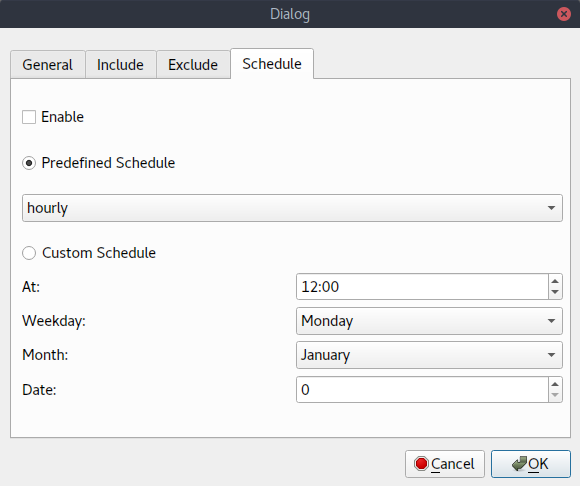
\includegraphics[width=.9\linewidth]{pictures/borgqt_settings_schedule.png}
\caption{\label{fig:org4597de1}
Screenshot der "`Schedule"' Einstellungen}
\end{figure}

Das Erstellen der eigentlichen Systemd Konfiguration passiert in Borg-Qt in der
\texttt{Config} Klasse zum gleichen Zeitpunkt, wie die eigentliche Konfigurationsdatei
geschrieben wird. Zum Schreiben und he-/aktivieren des Systemd Services,
respektive Timers wurde eine Klasse \texttt{SystemdFile} erstellt. Somit könnte
die Funktion auch einfach in einem anderen Projekt verwendet werden.

Systemd benötigt zum Starten der Anwendung den absoluten Pfad in der Service
Datei. Da davon ausgegangen werden kann das Borg-Qt im \texttt{PATH} des Systems
abgelegt wird, wurde das Unix Tool "`which"' verwendet um den exakten Speicherort
zu erhalten. Mittels des Befehls \texttt{which borg-qt} erhält man den absoluten
Speicherort der Datei. Zusammen mit den Daten aus den Einstellungen wird diese
Information in einem \texttt{Configparser} Objekt gespeichert, welches dann mithilfe
der \texttt{SystemdFile} Klasse in eine \texttt{borg\_qt.service},
Codesnippet:(\ref{org15aed53}), respektive \texttt{borg\_qt.timer},
Codesnippet:(\ref{orgcc10efb}), Datei, im Systemd Pfad
\texttt{/home/username/.config/systemd/user/} geschrieben und aktiviert wird.

Eine Option in der Datei \texttt{borg\_qt.timer} die noch erwähnenswert ist, ist
\texttt{Persistent = true}. Ist \texttt{Persistent} auf \texttt{true} gesetzt, holt Systemd den
Tasks nach sollte er eine Ausführung verpasst haben. Dies ist insbesondere dann
hilfreich, wenn etwa der Zeitplan auf \texttt{daily} oder \texttt{weekly} gesetzt wurde.
Sollte also etwa jeden Mittwoch ein Backup gemacht werden aber der Computer
lief an diesem Tag nicht, startet Systemd Borg-Qt, sobald der Computer das
nächste Mal eingeschaltet wird kommt.

Mit dem Abschluss des automatischen Backups wurde die für die Entwicklung
reservierte Zeit aufgebraucht und die Entwicklung neuer Funktionen für den
Zeitrahmen der Diplomarbeit gestoppt.

\lstset{language=bash,label=org15aed53,caption={Systemd Service Datei für Borg-Qt},captionpos=b,numbers=none}
\begin{sexylisting}{Systemd Service Datei für Borg-Qt}
#~/.config/systemd/user/borg_qt.service
[Unit]
Description = Runs Borg-Qt once in the backround to take a backup according to the configuration.

[Service]
Type = oneshot
ExecStart = /home/andreas/bin/borg_qt -B
\end{sexylisting}

\lstset{language=bash,label=orgcc10efb,caption={Systemd Timer Datei für Borg-Qt},captionpos=b,numbers=none}
\begin{sexylisting}{Systemd Timer Datei für Borg-Qt}
#~/.config/systemd/user/borg_qt.timer
[Unit]
Description = Starts the borg_qt.service according to the configured schedule.

[Timer]
OnCalendar = hourly
Persistent = true

[Install]
WantedBy = timers.target
\end{sexylisting}

\subsection{\gls{gui} Anpassungen nach Benutzerfreundlichkeitsstudie}
\label{sec:orgd36c09f}

Im Rahmen der durchgeführten \hyperref[sec:orgbeaa226]{Benutzerfreundlichkeitsstudie} wurden einige Punkte
festgestellt, welche im Rahmen der Diplomarbeit angepasst werden konnten. Zum
einen wurden in den "`Include"' sowie "`Exclude"' Optionen einige Buttons neu
beschriftet und zwei Labels hinzugefügt, um klarer auf ihre Funktion
hinzuweisen. Zu sehen ist dies in den
Abbildungen:(\ref{fig:orgf92bace}) und
(\ref{fig:orgd3a5abe}).

\begin{figure}[H]
\centering
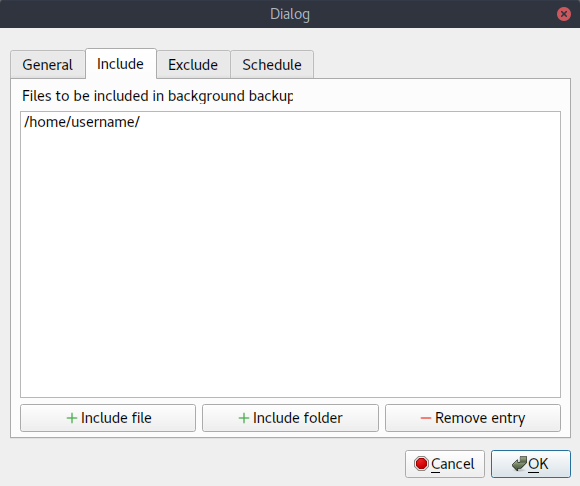
\includegraphics[width=.9\linewidth]{pictures/borgqt_settings_include_v2.png}
\caption{\label{fig:orgf92bace}
Screenshot der Borg-Qt "`Include"' Einstellungen Version 2}
\end{figure}

\begin{figure}[H]
\centering
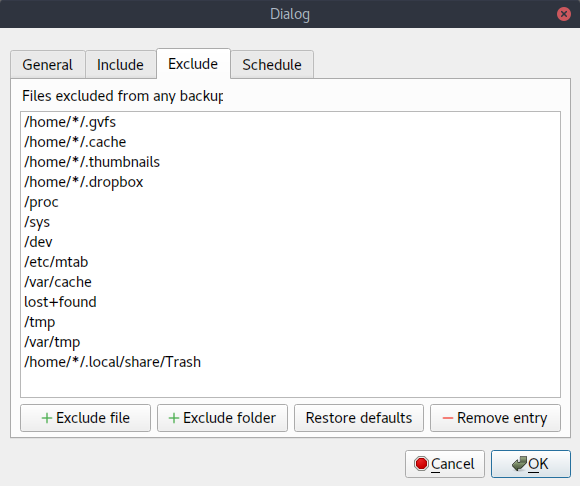
\includegraphics[width=.9\linewidth]{pictures/borgqt_settings_exclude_v2.png}
\caption{\label{fig:orgd3a5abe}
Screenshot der Borg-Qt "`Exclude"' Einstellungen Version 2}
\end{figure}

Zudem wurde ein Hilfe Fenster, Abbildung:(\ref{fig:orgc99d9b5}), eingebaut, welches
dem Benutzer beim Start der Applikation angezeigt wird. Dieses soll ihm einen
kurzen Überblick darüber geben, welcher Button welche Aktion auslöst und welche
Elemente, welche Information anzeigen. Optional kann der Benutzer noch
entscheiden, dass er das Fenster beim nächsten Start nicht mehr angezeigt
bekommen möchte. Über den Button "`Help"' kann das Fenster jederzeit unabhängig
der Einstellungen wieder angezeigt werden.

\begin{figure}[H]
\centering
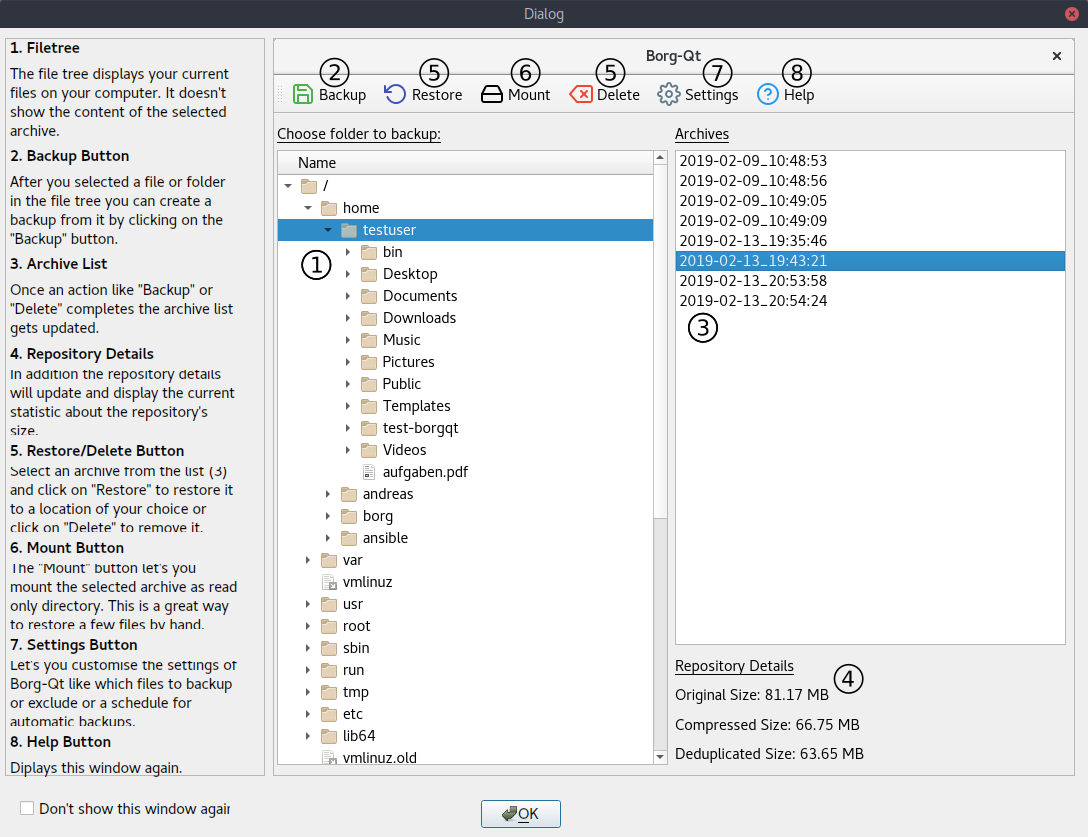
\includegraphics[width=.9\linewidth]{pictures/borgqt_help.png}
\caption{\label{fig:orgc99d9b5}
Screenshot des Borg-Qt Hilfe Fenster}
\end{figure}

\subsection{Releases}
\label{sec:orgf056008}

Für die finale Veröffentlichung wird Borg-Qt als ein sogenanntes ausführbares
"`Binary"' zur Verfügung gestellt. Man kennt diese auf Windows Systemen etwa als
die Dateien mit der Endung \texttt{.exe}. In diesem Fall handelt es sich beim Binary
um ein selbst entpackendes Dateiarchiv. Darin enthalten sind alle benötigten
Python Module und sonstige Dateien wie etwa die Icons oder \gls{gui}
Definitionsdateien. Beim Ausführen entpackt sich das Archiv in einen temporären
Ordner und liest dann von dort aus alle benötigten Dateien.

Diese Art der Auslieferung hat dabei den Vorteil, das der User das Programm
nicht speziell installieren muss oder dafür irgendwelche zusätzlichen Dinge
installieren muss. Der Nachteil ist jedoch das so ein Binary nur auf dem
jeweiligen Betriebssystem erstellt und ausgeführt werden kann. Das heisst das
man unter Linux etwa keine Binaries für Mac erstellen kann oder umgekehrt.

Erstellt werden die Dateien mit einem Programm namens
"`PyInstaller"'\footcite{pyinstaller}. Man führt das Programm dabei auf der
Kommandozeile gegen die Hauptdatei des Codes aus. Der Befehl dafür ist relativ
einfach, Codesnippet:(\ref{org688526f}). Wichtig dabei ist das man die Pfade
der zusätzlichen Dateien wie etwa Icons mit angibt da PyInstaller diese nicht
selber finden kann. Der gezeigte Code wurde dabei in ein Makefile
implementiert. Somit kann man in der obersten Ebene des Repository einfach den
Befehl \texttt{make} ausführen und das Binary wird im Ordner \texttt{dist} erstellt.

\lstset{language=bash,label=org688526f,caption={Code zum Erstellen der finalen Binaries von Borg-Qt},captionpos=b,numbers=none}
\begin{sexylisting}{Code zum Erstellen der finalen Binaries von Borg-Qt}
pyinstaller --hidden-import=PyQt5.sip \
    --add-data=borg_qt/static/icons:static/icons \
    --add-data=borg_qt/static/UI:static/UI \
    -F borg_qt/borg_qt.py; \
\end{sexylisting}

Auf Github wird jeweils ein Release erstellt und dazu die passenden Binaries
hochgeladen. Github packt dabei den Source Code beim Erstellen des Releases in
ein Zip Archiv. Somit kann eine interessierte Person sich zum Binary auch
direkt den Source Code herunterladen.

\section{Ausblick}
\label{sec:orge04eb5c}
\subsection{Erreichte Ziele}
\label{sec:org4cab61e}

\begin{center}
\begin{tabular}{lll}
Ziel Nr. & Erfüllt & Bemerkung\\
\hline
 &  & \\
\end{tabular}

\end{center}


\subsubsection{Risikoanalyse der neuen Ist-Situation}
\label{sec:org17afb77}

Das Risiko konnte massgeblich gesenkt. Mit den automatischen Backups gibt es nun
auch eine Möglichkeit das Vergessen zu minimieren.

\begin{figure}[htbp]
\centering
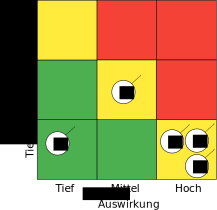
\includegraphics[width=.9\linewidth]{pictures/ist_risiko_neu.pdf}
\caption{\label{fig:org9de82f4}
Risikoanalyse der neuen Ist-Situation}
\end{figure}

\subsection{Projektmanagement}
\label{sec:orge9ec95b}

Gantt Chart sehr hilfreich beim behalten des Überblickes für das Projekt. Gibt
einem einen durchgehenden roten Faden.

Die konservativen Zeitschätzungen haben sich als korrekte Entscheidung
erwiesen. In Zukunft kann noch stärker versucht werden die Zeit welche für
ähnliche Code Teile verwendet wird kürzer zu schätzen. Copy/Paste erlaubt unter
Umständen enorme Zeitersparnise.

Die regelmässigen Arbeitsessions haben sich als eine gute Variante des Arbeiten
erwiesen und haben die Last der Diplomarbeit gut verteilt.

\subsection{Benutzerfreundlichkeitsstudie}
\label{sec:orgaf652d4}

Die Studie war eine sehr interessante Erfahrung. Enduser sehen eine
Anwendung mit ganz anderen Augen als der Entwickler der Anwendung der von jedem
Element weiss wie der Code dazu aussieht. Er hat auch gezeigt das die Aufgaben
auch richtig gestellt werden müssen ansonsten wissen die Probanden schon gar
nicht erst was gefordert ist. Auch sollte wenn möglich darauf geachtet werden
das auf einem Betriebsystem getestet mit welchem die Probanden bereits etwas
Erfahrung haben. Zwei der Probanden waren ab dem Verhalten und Aussehen des
Dateimanagers von Ubuntu 18.04 etwas verwirrt da sie ihn zuvor noch nicht
gesehen und bentuzt hatten. Alternativ kann auch die Gruppe der Probanden so
gewählt werden das sie mit dem Betriebssystem bereits vertraut sind.
Auf jeden Fall etwas was man bei zukünftigen Projekten wieder machten sollte.

\subsection{Umsetzung}
\label{sec:org6c2669d}

Aus zeitlichen Gründen konnte die Funktion zur Erkennung eines laufenden
Hypervisors nicht während der Diplomarbeit entwickelt werden. Dies ist ein
recht komplexes Features und braucht genügend Zeit damit es richtig umgesetzt
wird.

Unittests sind der Shit brauchen allerdings Zeit und eine gewisse Erfahrung mit
der Sprache. Qt ist eine hilfreiches Framework wenn auch sehr umfangreich. Wenn
man gewillt ist sich mit dem C++ Code auseinanderzusetzen ist die Dokumentation
jedoch sehr detailiert.

\subsection{Weiterverwendung von Borg-Qt}
\label{sec:org31bcde8}

Wird bereits produktiv vom Projektleiter eingesetzt.

\subsection{Gelerntes}
\label{sec:orgf621d2e}

PLACEHOLDER

\newpage
\begin{landscape}

\section{Anhang}
\label{sec:orgac7c4ec}

\subsection{Testfälle}
\label{sec:orgba12376}
{\footnotesize
\begin{longtable}{|>{\columncolor[HTML]{EFEFEF}}l|p{2cm}|p{2cm}|p{3.5cm}|p{2cm}|p{3cm}|p{3.5cm}|p{2.5cm}|}
\hline
\textbf{ID}\cellcolor[HTML]{C0C0C0} & \textbf{Objective}\cellcolor[HTML]{C0C0C0} & \textbf{Precondition}\cellcolor[HTML]{C0C0C0} & \textbf{Steps}\cellcolor[HTML]{C0C0C0} & \textbf{Testdata}\cellcolor[HTML]{C0C0C0} & \textbf{Expected Result}\cellcolor[HTML]{C0C0C0} & \textbf{Postcondition}\cellcolor[HTML]{C0C0C0} & \textbf{Result}\cellcolor[HTML]{C0C0C0}\\
\hline
\endfirsthead
\multicolumn{8}{l}{Fortsetzung von vorheriger Seite} \\
\hline

\textbf{ID}\cellcolor[HTML]{C0C0C0} & \textbf{Objective}\cellcolor[HTML]{C0C0C0} & \textbf{Precondition}\cellcolor[HTML]{C0C0C0} & \textbf{Steps}\cellcolor[HTML]{C0C0C0} & \textbf{Testdata}\cellcolor[HTML]{C0C0C0} & \textbf{Expected Result}\cellcolor[HTML]{C0C0C0} & \textbf{Postcondition}\cellcolor[HTML]{C0C0C0} & \textbf{Result}\cellcolor[HTML]{C0C0C0} \\

\hline
\endhead
\hline\multicolumn{8}{r}{Fortsetzung nächste Seite} \\
\endfoot
\endlastfoot
\hline
\textbf{TC-01} & Anwendung starten & Lokales Repository initialisiert.\newline Lokale Konfigurationsdatei erstellt. & 1. Anwendung starten. & - & Die Anwendung startet ohne Fehlermeldung und zeigt eine leere Backup Liste an. & Die Anwendung wird angezeigt. & Erfolgreich durchgeführt 25.02.2019 A.Z.\\
\hline
\textbf{TC-02} & Anwendung starten & Lokale Konfigurationsdatei erstellt. & 1. Anwendung starten. & - & Die Anwendung wirft eine Fehlermeldung das sie das lokale Repository nicht finden kann. & Die geöffnete Fehlermeldung blockiert die Applikation. & Erfolgreich durchgeführt 25.02.2019 A.Z.\\
\hline
\textbf{TC-03} & Anwendung starten & - & 1. Anwendung starten. & - & Die wirft eine Fehlermeldung das sie die Konfigurationsdatei nicht finden kann. & Die geöffnete Fehlermeldung blockiert die Applikation. & Erfolgreich durchgeführt 25.02.2019 A.Z.\\
\hline
\textbf{TC-04} & Lokales Backup erstellen & TC-01 ausgeführt. & 1. In der Ordnerübersicht das Code Repository auswählen.\newline 2. Den Button “Backup” betätigen. & Testdateien & Die Anwendung zeigt einen Fortschrittsbalken der nach erfolgreichem Backupen verschwindet. & Die Archiv Liste wird aktualisiert und zeigt ein Archiv an. & Erfolgreich durchgeführt 25.02.2019 A.Z.\\
\hline
\textbf{TC-05} & Lokales Backup erstellen & TC-01 ausgeführt.\newline \gls{borg} erstellt bereits ein Archiv. & 1. In der Ordnerübersicht das Code Repository auswählen.\newline 2. Den Button “Backup” betätigen. & Testdateien & Die Anwendung wirft eine Fehlermeldung das \gls{borg} bereits ausgeführt wird. & Die geöffnete Fehlermeldung blockiert die Applikation. & Erfolgreich durchgeführt 25.02.2019 A.Z.\\
\hline
\textbf{TC-06} & Lokales Backup erstellen & TC-01 ausgeführt. & 1. Das Lokale Repository an einen beliebigen Ort verschieben.\newline 2. In der Ordnerübersicht das Code Repository auswählen.\newline 3. Den Button “Backup” betätigen. & Testdateien & Die Anwendung wirft eine Fehlermeldung das sie das lokale Repository nicht finden kann. & Die geöffnete Fehlermeldung blockiert die Applikation. & Erfolgreich durchgeführt 25.02.2019 A.Z.\\
\hline
\textbf{TC-07} & In lokales Repository sichern & TC-01 ausgeführt. & 1. Den Button “Backup” betätigen. & - & Die Anwendung wirft eine Fehlermeldung das der User einen Pfad angeben soll. & Die geöffnete Fehlermeldung blockiert die Applikation. & Erfolgreich durchgeführt 25.02.2019 A.Z.\\
\hline
\textbf{TC-08} & Lokales Archiv löschen & TC-04 ausgeführt. & 1. In der Backup Liste das Backup auswählen.\newline 2. Den Button “Delete” betätigen. & - & Die Anwendung zeigt einen Fortschrittsbalken der nach erfolgtem Löschen verschwindet. & Die Archiv Liste wird aktualisiert und ist nun leer. & Erfolgreich durchgeführt 25.02.2019 A.Z.\\
\hline
\textbf{TC-09} & Lokales Archiv löschen & TC-04 ausgeführt. & 1. Das Lokale Repository an einen beliebigen Ort verschieben.\newline 2. In der Archiv Liste das Archiv auswählen.\newline 3. Den Button “Delete” betätigen. & - & Die Anwendung wirft eine Fehlermeldung das sie das lokale Repository nicht finden kann. & Die geöffnete Fehlermeldung blockiert die Applikation. & Erfolgreich durchgeführt 25.02.2019 A.Z.\\
\hline
\textbf{TC-10} & Lokales Archiv löschen & TC-04 ausgeführt. & 1. Den Button “Delete” betätigen. & - & Die Anwendung wirft eine Fehlermeldung das der User ein Archiv auswählen soll. & Die geöffnete Fehlermeldung blockiert die Applikation. & Erfolgreich durchgeführt 25.02.2019 A.Z.\\
\hline
\textbf{TC-11} & Lokales Archiv wiederherstellen & TC-04 ausgeführt. & 1. In der Archiv Liste das Archiv auswählen.\newline 2. Den Button “Restore” betätigen.\newline 3. Im geöffneten Dateidialog den Pfad "`/home/andreas/Downloads"' auswählen.\newline 4. Den Button “Open” anklicken. & - & Nach erfolgtem Wiederherstellen öffnet ein Dateiexplorer den Ziel Pfad. & Die Anwendung und ein Dateiexplorer wird angezeigt. & Erfolgreich durchgeführt 25.02.2019 A.Z.\\
\hline
\textbf{TC-12} & Lokales Archiv wiederherstellen & TC-01 ausgeführt. & 1. Den Button “Backup” betätigen. & - & Die Anwendung wirft eine Fehlermeldung das der User ein Archiv auswählen soll. & Die geöffnete Fehlermeldung blockiert die Applikation. & Erfolgreich durchgeführt 25.02.2019 A.Z.\\
\hline
\textbf{TC-13} & Lokales Archiv wiederherstellen & TC-01 ausgeführt. & 1. Das Lokale Repository an einen beliebigen Ort verschieben.\newline 2. In der Archiv Liste das Archiv auswählen.\newline 3. Den Button “Restore” betätigen. & - & Die Anwendung wirft eine Fehlermeldung das sie das lokale Repository nicht finden kann. & Die geöffnete Fehlermeldung blockiert die Applikation. & Erfolgreich durchgeführt 25.02.2019 A.Z.\\
\hline
\textbf{TC-14} & Lokales Archiv wiederherstellen & TC-01 ausgeführt. & 1. In der Archiv Liste das Archiv auswählen.\newline 2. Den Button “Restore” betätigen.\newline 3. Im geöffneten Dateidialog den Pfad "`/home/andreas/Downloads"' auswählen.\newline 4. Den Button “Cancel” anklicken. & - & Der Datei Dialog schliesst sich wieder. & Die Anwendung wird angezeigt. & Erfolgreich durchgeführt 25.02.2019 A.Z.\\
\hline
\textbf{TC-15} & Home Directory sichern und wiederherstellen & TC-01 ausgeführt. & 1. Vom Pfad "`\emph{home/andreas}"' ein Archiv erstellen.\newline 2. In der Archiv Liste das gemachte Archiv auswählen.\newline 3. Den Button “Restore” betätigen.\newline 4. Im geöffneten Dateidialog den Pfad "`/home/andreas/Downloads"' auswählen.\newline 5. Den Button “Open” anklicken. & "`\emph{home/andreas}"' & Nach erfolgtem Wiederherstellen öffnet ein Dateiexplorer den Ziel Pfad.\newline Darin fehlen jedoch temporäre Pfade wie “\textasciitilde{}/.cache” etc. & Die Anwendung und ein Dateiexplorer wird angezeigt. & Erfolgreich durchgeführt 25.02.2019 A.Z.\\
\hline
\textbf{TC-16} & Einzelne Datei wiederherstellen & TC-04 ausgeführt. & 1. In der Backup Liste das Backup auswählen.\newline 2. Den Button “Mount” betätigen.\newline 3. Aus dem sich öffnenden Dateiexplorer die Datei README.org nach "`/home/andreas/Downloads"' kopieren. & - & Die wiederhergestellte Datei ist identisch mit der in TC-04 gesicherten. & Die Anwendung und ein Dateiexplorer wird angezeigt. & Erfolgreich durchgeführt 25.02.2019 A.Z.\\
\hline
\textbf{TC-17} & Einzelne Datei wiederherstellen & TC-01 ausgeführt. & 1. Das Lokale Repository an einen beliebigen Ort verschieben.\newline 2. In der Archiv Liste das Archiv auswählen.\newline 3. Den Button “Mount” betätigen. & - & Die Anwendung wirft eine Fehlermeldung das sie das lokale Repository nicht finden kann. & Die geöffnete Fehlermeldung blockiert die Applikation. & Erfolgreich durchgeführt 25.02.2019 A.Z.\\
\hline
\textbf{TC-18} & Pfad des lokalen Backup Repository anpassen & TC-04 ausgeführt.\newline Backup Repository nach "`/tmp/test-borgqt2"' verschoben & 1. Den Button "`Settings"' betätigen.\newline 2. Den Repository Pfad auf "`\emph{tmp/test-borgqt2}"' ändern.\newline 3. Den Button "`Apply"' betätigen. & - & Die Archiv Liste wird aktualisiert und zeigt wieder das Archiv von TC-04 an. & Die Anwendung wird angezeigt. Die Konfigurationsdatei zeigt auf den neuen Pfad. & Nicht implementiert\\
\hline
\textbf{TC-19} & Archiv Name ändern & TC-01 ausgeführt. & 1. Den Button "`Settings"' betätigen.\newline 2. Bei der Option "`Archive Prefix"' "`Muster"' eintragen.\newline 3. Den Button "`Apply"' betätigen.\newline 4. TC-04 durchführen. & Archiv Name: Muster & Die Anwendung zeigt einen Fortschrittsbalken der nach erfolgtem Backup verschwindet. & Die Archiv Liste wird aktualisiert und zeigt ein Archiv mit dem Präfix "`Muster"' an. Die Konfigurationsdatei beinhaltet die Option des Präfixes. & Erfolgreich durchgeführt 25.02.2019 A.Z.\\
\hline
\textbf{TC-20} & Keine Einstellungen ändern & TC-01 ausgeführt. & 1. Den Button "`Settings"' betätigen.\newline 2. Eine beliebige Option ändern.\newline 3. Den Button "`Cancel"' betätigen. & - & Der Einstellungsdialog schliesst sich. & Die Anwendung wird angezeigt. Die Konfigurationsdatei ist noch im selben Zustand wie bei TC-01. & Erfolgreich durchgeführt 25.02.2019 A.Z.\\
\hline
\textbf{TC-21} & Automatische Backups konfigurieren & TC-01 ausgeführt. & 1. Den Button "`Settings"' betätigen.\newline 2. Bei der Option "`Includes"' die Testdateien angeben sowie unter Schedule "`Custom"' auswählen und bei "`Time"' die nächste Stunde angeben.\newline 3. Den Button Apply betätigen. & Backup-zeit: 2 Minuten nach aktueller Zeit Testdateien & Der Datei Dialog schliesst sich wieder. & Die Anwendung wird angezeigt. Die Konfigurationsdatei wurde um die Option des automatischen Backups erweitert. Die Anwendung hat einen "`Service"' auf dem System erstellt. & Erfolgreich durchgeführt 25.02.2019 A.Z.\\
\hline
\textbf{TC-22} & Automatische Backups durchführen & TC-16 ausgeführt. & 1. TC-21 durchführen.\newline 2. Auf Ablauf der Zeit warten.\newline 3. Die Anwendung öffnen. & - & In der Archiv Liste wird ein Archiv angezeigt. & Die Anwendung wird angezeigt. & Erfolgreich durchgeführt 25.02.2019 A.Z.\\
\hline
\textbf{TC-23} & Server Archiv erstellen & Server Repository bereit.\newline Server Konfigurationsdatei erstellt. & TC-04 durchführen. & Testdateien & Die Anwendung zeigt einen Fortschrittsbalken der nach erfolgtem Backup verschwindet. & Die Archiv Liste wird aktualisiert und zeigt ein Archiv an. & Erfolgreich durchgeführt 25.02.2019 A.Z.\\
\hline
\textbf{TC-24} & Lokales Archiv erstellen während dem eine VM läuft & TC-01 ausgeführt.\newline Virtualbox VM Starten. & 1. In der Ordnerübersicht das Code Repository auswählen.\newline 2. Den Button “Backup” betätigen. & Testdateien & Die Anwendung wirft eine Fehlermeldung aus das es zur Zeit aufgrund einer laufenden VM unsicher sei ein Backup durchzuführen. & Die geöffnete Fehlermeldung blockiert die Applikation. & Nicht implementiert\\
\hline
\textbf{TC-25} & Abgebrochenes Backup bereinigen & TC-01 ausgeführt. & 1. In der Ordnerübersicht das Code Repository auswählen.\newline 2. Den Button “Backup” betätigen.\newline 3. Die Anwendung schliessen.\newline 4. Anwendung wieder öffnen.\newline 5. TC-04 Durchführen. & Testdateien & Bei Schritt 4. sollte ein Teilarchiv zu sehen sein.\newline Bei Schritt 5 sollte einfach ein normales Archiv zu sehen sein. & Die Anwendung wird angezeigt. & Erfolgreich durchgeführt 25.02.2019 A.Z.\\
\hline
\caption{\label{tab:orgd13fe87}
Testfälle}
\\
\end{longtable}
}
\end{landscape}

\newpage
\begin{landscape}
\subsection{Klassendiagramm}
\label{sec:org213e886}
\begin{figure}[H]
\centering
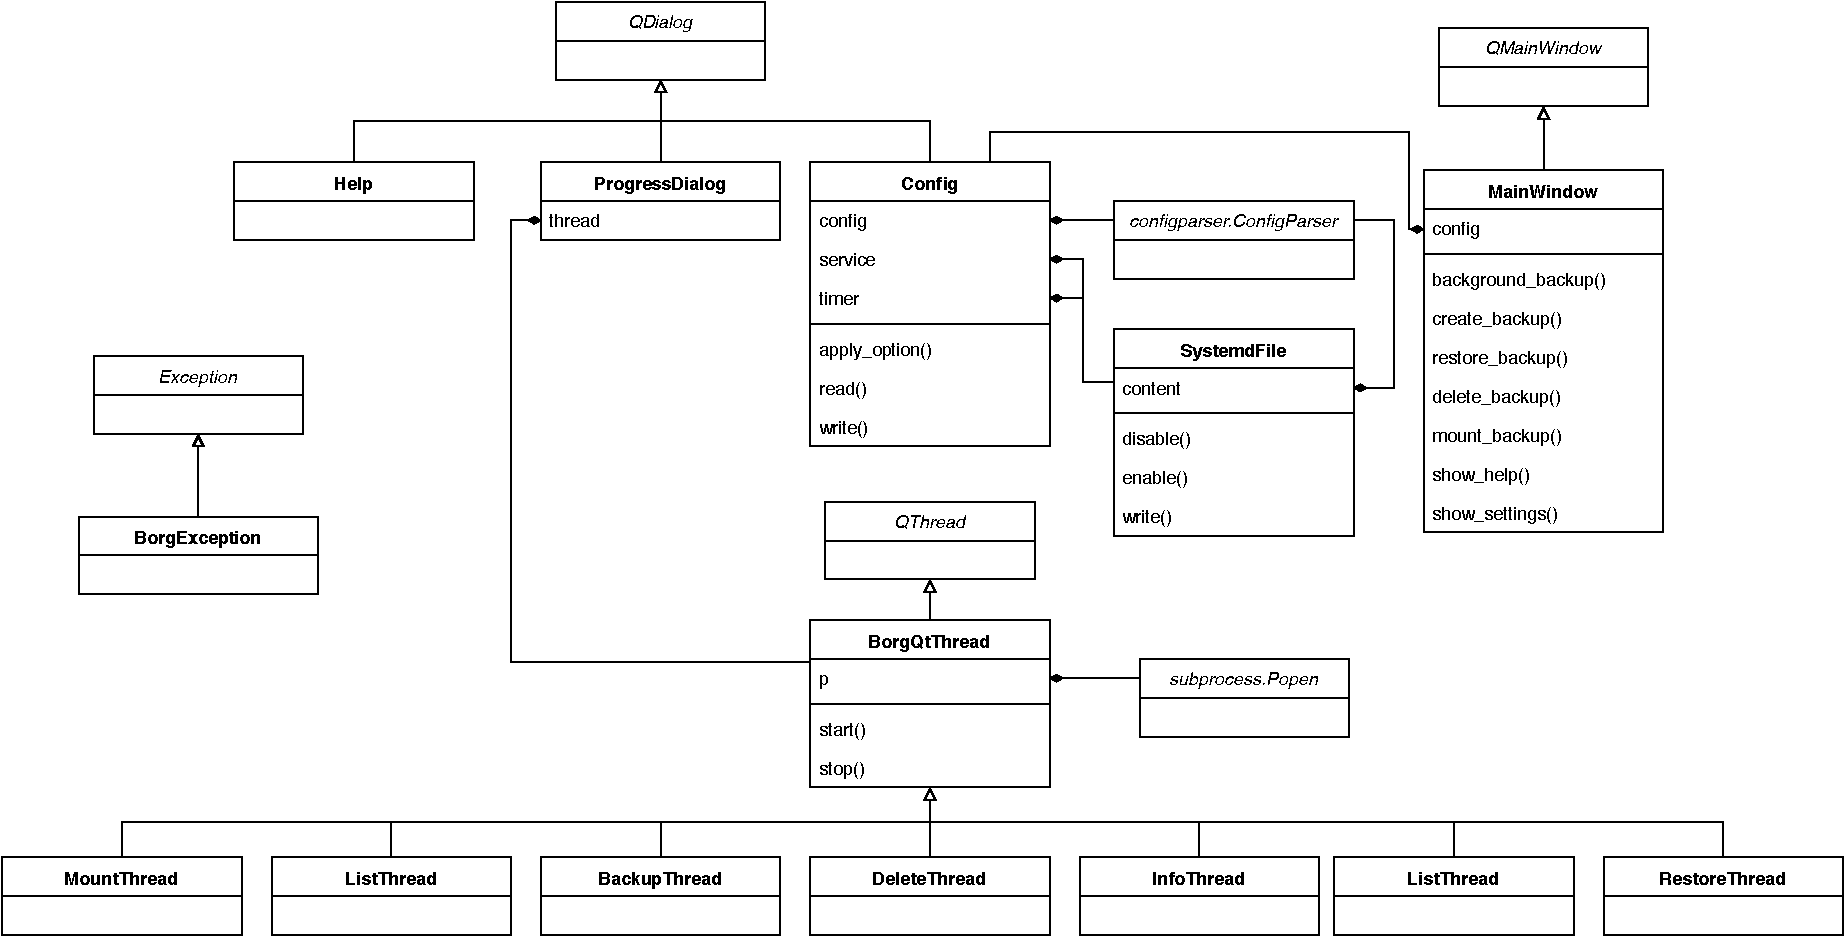
\includegraphics[height=.7\textwidth]{pictures/class_diagramm.pdf}
\caption{\label{fig:org4ac1491}
Klassendiagramm der Borg-Qt Applikation}
\end{figure}
\end{landscape}

\newpage
\begin{landscape}
\subsection{Arbeitsjournal}
\label{sec:orga5f85b1}

\begin{longtable}{|p{2cm}|p{5cm}|p{5cm}|p{7cm}|}
\hline
\textbf{Von/Bis}\cellcolor[HTML]{C0C0C0} & \textbf{Geplante Arbeiten}\cellcolor[HTML]{C0C0C0} & \textbf{Erreichte Arbeiten}\cellcolor[HTML]{C0C0C0} & \textbf{Eindruck}\cellcolor[HTML]{C0C0C0}\\
\hline
\endfirsthead
\multicolumn{4}{l}{Fortsetzung von vorheriger Seite} \\
\hline

\textbf{Von/Bis}\cellcolor[HTML]{C0C0C0} & \textbf{Geplante Arbeiten}\cellcolor[HTML]{C0C0C0} & \textbf{Erreichte Arbeiten}\cellcolor[HTML]{C0C0C0} & \textbf{Eindruck}\cellcolor[HTML]{C0C0C0} \\

\hline
\endhead
\hline\multicolumn{4}{r}{Fortsetzung nächste Seite} \\
\endfoot
\endlastfoot
\hline
10.-16.12.2018 & Zeitplan erarbeiten, Ziele dokumentieren & keine Abweichung & -\\
\hline
17.-23.12.2018 & Lösungsvarianten erfassen, Lösungsvarianten bewerten, Lösungsvariante bestimmen, SWOT Analyse erstellen, 1. Meeting & keine Abweichung & Marco Frei hat noch diverse Punkte eingebracht die, die Planung ziemlich durcheinander bringen. Bedeute viel zusätzliche Arbeit.\\
\hline
24.-30.12.2018 & Controlling erarbeiten, Ist- und Soll-Analyse, SWOT Analyse, Umweltanalyse, Massnahmen Katalog erarbeiten, User Stories erarbeiten, Use Case Diagramm erstellen, Use Cases ausarbeiten, Anforderungskatalog erstellen, UML Diagramme & keine Abweichung & UML Diagramme für eine Software zu erstellen die nicht existiert ist noch eine interessante Herausforderung.\\
\hline
31.12-06.01.2019 & Lösungsvarianten erarbeiten und entscheiden, Test Konzept beschreiben und Testfälle erstellen, Github Repository erstellen & Testfälle liessen sich noch nicht für alle Ziele erstellen. Gewisse Features hängen noch sehr davon ab wie die Basis der Applikation sich entwickelt. & Insgesamt gut gelaufen. Das Repository auf Github konnte ich unter einer eigenen Organisation erstellen dadurch wird das Zusammenarbeiten in der Zukunf einfacher.\\
\hline
07.-13.01.2019 & UI ausarbeiten, UI Test ausarbeiten & keine Abweichung & Das das Projekt gut im Zeitplan ist soweit ein positiver Ausblick.\\
\hline
14.-20.01.2019 & Backend "`Read Config"' Funktion schreiben, Frontend "`Read Config"'  Funktion beginnen & "`Frontend Read Config"', "`Backend Write Config"', "`Frontend Write Config"', Funktion bereits abgeschlossen. & Soweit sehr gut im Zeitplan. Die Arbeitssessions mit den Kollegen helfen. Seltsam das Qt keine Methode list.items() kennt.\\
\hline
21.-27.01.2019 & "`Backend Backup"' Funktion, "`Frontend Backup"' Funktion beginnen, Automatische Backups recherchieren & keine Abweichung & Erkältung drückt etwas auf die Performance. Unittest sind nocht nicht perfekt aber sind eine grosse Hilfe.\\
\hline
28.-03.02.2019 & "`Frontend Backup"' Funktion fertigstellen, "`Backend und Frontend Restore"' Funktion & Geplantes erreicht sowie "`Mounting"' und "`Delete"' Funktion sowohl im Backend wie auch im Frontend bereits umgesetzt. & Da die Funktionen immer von \gls{borg} ausgeführt werden konnte sehr viel Code von den "`Backup"' und "`Restore"' Funktionen übernommen werden was die Entwicklung sehr beschleunigt hat.\\
\hline
04.02.-10.02.2019 & Meeting Pendenzen nochmal durchgehen. Die Interface Funktionen bereinigen. Automatische Backups implementieren. & Meeting Pendenzen wurden aufgenommen und das Interface wurde bereinigt. Automatische Backups konnten noch nicht fertig gestellt werden. & Automatische Backups sind noch relativ komplex und benötigen Kenntnisse der Systemd Timer.\\
\hline
11.02.-17.02.2019 & UI Tests mit den Usern durchführen, Resultate auswerten, Feedback in Applikation einarbeiten & keine Abweichung & Es ist sehr spannend zu sehen wie Benutzer mit der Anwendung interagieren und welche Featues sie vermissen.\\
\hline
18.02.-24.02.2019 & Automatische Backups implementieren, 1. Release veröffentlichen, Readme updaten & keine Abweichung & Das Projekt ist soweit sehr gut im Zeitplan. Die Systemd Timer sind können mit vielen verschiedenen Zeitformaten umgehen und sind sehr flexibel.\\
\hline
25.02.-03.03.2019 & Testfälle durchgehen, Dokumentation zur Realisierung abschliessen &  & \\
\hline
\caption{\label{tab:orgb33e26b}
Arbeitsjournal}
\\
\end{longtable}
\end{landscape}
